\documentclass[12pt]{article}
\usepackage[spanish, english, es-tabla]{babel}
\usepackage[utf8]{inputenc}
\usepackage{amsmath,amssymb}
\usepackage{graphicx}
\usepackage{gensymb}
\usepackage{outlines}
\usepackage[export]{adjustbox}
\usepackage{adjustbox}
\usepackage{multicol}
\usepackage{lipsum}
\parskip 1ex

\usepackage{eurosym}

% add code
\usepackage{listings}

\usepackage{array}

% text font 

\usepackage{courier}

%\usepackage{fontspec}

\usepackage[dvipsnames]{xcolor}

\usepackage{hyperref}
\usepackage{subcaption}
\usepackage[left = 2cm, right = 2cm, bottom = 2cm, top = 3cm]{geometry}

\hypersetup{
	colorlinks=true,
	linkcolor=black,
	%filecolor=magenta,      
	urlcolor=cyan,
}

\hypersetup{
	pdftitle= {Diseño y automatización de un sistema de alimentación OpenSource para animales a través de la tecnología LoRa},
	pdfauthor = {Lucía Francoso Fernández},
	pdfsubject = {Electrónica y comunicaciones móviles},
	pdfkeywords = {Arduino, LoRa, automatización, LoRaWAN, punto a punto, OpenSource}
}

% define color for C code (Anexos)

\definecolor{codegreen}{rgb}{0,0.6,0}
\definecolor{codegray}{rgb}{0.5,0.5,0.5}
\definecolor{codepurple}{rgb}{0.58,0,0.82}
\definecolor{backcolour}{rgb}{0.95,0.95,0.92}

\lstdefinestyle{mystyle}{
	backgroundcolor=\color{backcolour},   
	commentstyle=\color{codegreen},
	keywordstyle=\color{magenta},
	numberstyle=\tiny\color{codegray},
	stringstyle=\color{codepurple},
	basicstyle=\ttfamily\footnotesize,
	breakatwhitespace=false,         
	breaklines=true,                 
	captionpos=b,                    
	keepspaces=true,                 
	numbers=left,                    
	numbersep=5pt,                  
	showspaces=false,                
	showstringspaces=false,
	showtabs=false,                  
	tabsize=2
}

\lstset{style=mystyle}

% https://tex.stackexchange.com/questions/60209/how-to-add-an-extra-level-of-sections-with-headings-below-subsubsection
\newcommand{\subsubsubsection}[1]{\paragraph{#1}\mbox{}\\}
\setcounter{secnumdepth}{4}
\setcounter{tocdepth}{4}

\begin{document}
	\selectlanguage{spanish}
	
	%\thispagestyle{empty}
	

	
	%\pagebreak
	
	\thispagestyle{empty}
	
	\newgeometry{left=0.01cm,bottom=0.01cm, top=0.01cm}
	
	%width=0.3\textwidth,
		
	%\begin{figure}[h!]
	%	
\includegraphics[height=\textheight,left]{img/banda_etsit_90.png}

%	\end{figure}

	\begin{minipage}{0.2\textwidth}
		
\includegraphics[height=\textheight,left]{img/banda_etsit_90.png}
	\end{minipage}
	\centerline{\begin{minipage}[t][5cm][b]{0.5\textwidth}
		%	\textbf{UNIVERSIDAD POLITÉCNICA DE} \\
			
		%	\textbf{CARTAGENA}\\
			
			\title{\textbf{Automatización y control de bebederos automáticos para especies animales usando LoRa}} 
			\maketitle
			
			\vspace{0.5cm}
			
			\hspace{1.5cm} \textbf{TRABAJO FIN DE GRADO} \\
			
			\vspace{0.5cm}
			
			\hspace{1.3cm} Grado en Ingeniería en Sistemas  de\\
			
			\vspace{0.01cm}
			
			\hspace{2.7cm} Telecomunicaciones \\
			
			\vspace{1cm}
			
			\textbf{Autora:}\author{ Lucía Francoso Fernández}\\
			
			\textbf{Tutor:} Juan Pascual García
		\end{minipage}}

	
	\restoregeometry
	
	\pagebreak
	
	\tableofcontents
	
	\pagebreak

	\listoffigures
	\addcontentsline{toc}{section}{Índice de figuras}
	
	\pagebreak
	
	\listoftables
	\addcontentsline{toc}{section}{Índice de tablas}
	
	\pagebreak
	
	\section*{Agradecimientos}
	\addcontentsline{toc}{section}{Agradecimientos}
	
	\noindent Primero, me gustaría agradecer a mi tutor, Juan Pascual García, por aceptar este reto junto a mi, y apoyarlo en todo momento. Fue un proyecto diferente, algo arriesgado, y siempre confió en que lo sacaríamos hacia delante. Muchas gracias por tu apoyo a distancia, debido a la Covid-19, que a pesar de todo siempre he obtenido tu ayuda y tu feedback a tiempo, y confianza en todo proceso requerido en este proyecto, pilares fundamentales en cualquier emprendimiento.\\
	
	\noindent Me gustaría, además, agradecer a mi familia, en especial a mis padres, Francisco y María Dolores, ya que es difícil entender que decida estar un año sin apenas créditos matriculados, la importancia de aprender de manera complementaria a la universidad, de buscar (y encontrar) aquello que me gusta dentro de esta carrera que, a pesar de las dificultades, siento que no podría haber elegido otra mejor. Sin ese apoyo, todo habría sido mucho más difícil, y siendo mi situación poco común, agradezco que lo hayan comprendido. A esto se suma su aportación económica, sin ella no habría podido realizar este proyecto, el cual he sentido en todo momento muy personal y muy bueno para mi, en tanto a nivel profesional, como personal como para la protectora que será beneficiaria de este dispositivo. Agradecer a mis hermanas Isabel y Claudia, que a pesar de las diferencias, y a pesar de ser la mayor, tienden a reforzarme en los momentos difíciles, recalcando mis virtudes; confiaron en este proyecto, y saben lo bueno que podría conllevar, ya que han venido innumerables veces conmigo al refugio, al igual que mi padre.\\
	
	\noindent También agradecer al resto de mi familia, que en la distancia también me apoyan. En especial a mi tía Bárbara, que siempre me llama para darme ánimos con todo lo que hago y que confía en mi desde siempre. A mis primas Sonia y María, y a mi abuela Guadalupe, las cuales son ejemplos de mujeres admirables en mi familia y a las que quiero muchísimo. Especial mención a mi abuela, Lucía Figueredo, la cual falleció el año pasado y sé que estaría muy orgullosa de ver a su nieta convertirse en ingeniera, y creando este proyecto. \\
	
	\noindent Debo agradecer también a mis suegros, Encarnación y Miguel Ángel, por dedicarme parte de su tiempo siempre que pueden, y en especial, en el desarrollo del prototipo exterior; agradezco enormemente que me hayan prestado sus herramientas, ya que sin ellas el resultado no habría sido el mismo. Muchas gracias por permitirme instalar en vuestra casa el otro extremo de la comunicación, que ha permitido poder concebir este proyecto. \\
	
	\noindent Me gustaría también agradecer a mi amiga Magdalena, mi amiga de toda la vida, la cual me apoya incondicionalmente, y me inspira en su lucha constante por mejorarse así misma y por ganarse la vida en lo que más le gusta, la música. A mi amiga Clara, la cual es una estupenda teleco, que siempre ha confiado en mi más que yo misma, y la cual me inspira por ser una persona fuerte, independiente y que tiene claro lo que quiere. A mi amigo Pablo, porque ni la distancia ni las exigentes carreras que cursamos nos han hecho perder el contacto, ni perder un vínculo que hace años se formó. Es un placer poder contar con estar tres personas.\\  
	
	\noindent Especial mención a mi compañero Enrique Fernández Sánchez, el cual ha sido también como mi tutor, ayudándome muchísimo a comprender la importancia del Open Source, guiándome en el conocimiento sobre microcontroladores y LoRa, y en general, aconsejándome en todo lo que ha podido y más. Gracias a él, la introducción al mundo maker se me ha hecho más sencilla, mucho más consciente y sin excesivos agobios. A esto, añadir que su aportación económica me ha ayudado muchísimo a sacar este proyecto hacia delante. Sin duda, ajeno a este proyecto, aprenderé muchas cosas de él y gracias a él, y no me cabe la menor duda de que es un gran teleco y una gran persona.\\
	
	\noindent Agradecer a Patitas Unidas Los Alcázares por permitirme instalar un dispositivo en sus instalaciones, y por comprender mi ausencia durante algunos meses donde el desarrollo de este proyecto era muy exigente. Especial mención a mi compañera Jen, con la que voy al refugio prácticamente siempre; sus ganas y actitud al tratar con los perros desde luego es una cualidad a admirar, y es una inspiración que recarga fuerzas para seguir luchando por los animales.\\
	
	\noindent Por último, agradecer a todas esas personas que han subido a la nube su proyecto, su documentación y dejan todo ese desarrollo bajo licencia Open Source, permitiendo que gente como yo desarrolle su proyecto basándome en sus librerías, o me den ideas que sin duda impulsen el mío. Estarán debidamente mencionadas, ya que merecen ese crédito.\\
	
	\pagebreak
	
	\section[Introducción]{Introducción} %corchetes, marcapaginas, llaves, texto
	
	Tras finalizar los estudios de grado en ingeniería en sistemas de telecomunicaciones, se requiere como último paso para la obtención del título la elaboración del \textit{Trabajo Fin de Grado} (TFG). 
	El TFG como tal tiene unos objetivos claros, los cuales son demostrar que se han adquirido las competencias básicas intrínsecas al grado, y que el alumno es capaz de seguir aprendiendo a partir de los conocimientos ya obtenidos, innovar, desenvolverse ante un problema determinado y, en resumen, saber llevar a cabo una investigación o proyecto que tenga como objetivo la resolución de dicho problema. \\
	
	\noindent En este documento, se recoge el proyecto realizado como TFG,  el cual va en línea con la filosofía y objetivos del \textit{Trabajo Fin de Grado} en sí mismo. Se detallará el proceso de creación de un sistema de alimentación para animales automatizado, donde se monitorizan de manera remota el estado de los tanques de reserva de agua y pienso. Así, se pretende exponer el conjunto de elementos hardware y software que serán necesarios para monitorizar, automatizar y acceder a ciertos datos de forma remota empleando, principalmente, Arduino y LoRa.\\
	
	
	\subsection[Contexto y justificación del trabajo]{Contexto y justificación del trabajo}
	\label{subsection: contexto y justificacion}
	
	\noindent Este proyecto ha sido concebido con el objetivo principal de ayudar a la preservación de la vida animal, ante el aumento de especies en extinción, sobre todo en lo que llevamos de siglo [\ref{bib: enlace National Geographic}]-[\ref{bib: enlace Fundación AQUAE}], 
	y ante el hecho de que miles de animales domésticos siguen siendo abandonados al año en España [\ref{bib: enlace Fundación Affinity}]-[\ref{bib: enlace RTVE}]. \\ %\footnotemark. \\
	
	%Fundación Affinity, 20 minutos, La Razón, RTVE
	%\footnotetext{\href{https://www.fundacion-affinity.org/observatorio/infografia-el-nunca-lo-haria-estudio-de-abandono-y-adopcion-2020}{Fundación Affinity}, \href{https://www.20minutos.es/noticia/4318383/0/el-abandono-animal-en-espana-aumenta-un-25-en-las-ultimas-semanas/}{20 minutos}, \href{https://www.larazon.es/medio-ambiente/20201118/qxv6yuokargfbnjvknn6bhm4ze.html}{La Razón}, \href{https://www.rtve.es/noticias/20200608/abandonos-animales-domesticos-se-han-disparado-espana-durante-meses-confinamiento/2015761.shtml}{RTVE}}

	\noindent Es por ello que se requiere de ayuda activa para paliar estos problemas. Las tareas de carácter solidario, en bastantes casos, no siempre cuentan con suficientes voluntarios; además, siendo un problema tan extendido y avanzado, el número de acciones que hay que llevar a cabo para aliviarlo es alto para un número limitado de voluntarios, los cuales deben incrementar considerablemente el tiempo que pasan realizando este tipo de tareas. 
	Tanto si se trata de un refugio de animales domésticos abandonados, como de reservas naturales donde se intenta repoblar una especie, los animales dependen enteramente del trabajo de los voluntarios. Así pues, es de vital importancia la optimización de las tareas de voluntariado, su automatización e, incluso, control remoto, mediante la creación de herramientas que ayuden a reducir el tiempo que se destina a tareas rutinarias para poder utilizar ese tiempo a otras tareas (de rescate, o de financiación para el mantenimiento de las instalaciones y de los propios animales, por ejemplo). \\
	
	\noindent Con el objetivo en mente de ayudar a la preservación de la fauna (y con ello, de la vida de los ecosistemas terrestres), evitando la extinción de especies y el abandono animal, se ha concebido y desarrollado este proyecto teniendo en cuenta los diferentes casos de uso (emplazamientos donde se podrá instalar el sistema, características del entorno), mejor adaptación a ellos, relación entre buenas prestaciones y bajo consumo, precio total del producto, o facilidad de uso por parte de un usuario medio. Es por ello que desde el principio se propone una serie de actuaciones a realizar, acorde a lo anteriormente mencionado, tales como: \\
	
	\begin{itemize}
		\item El diseño del sistema de alimentación será tal que el producto final pueda ser instalado no sólo en hogares, sino en sitios remotos, donde el acceso a recursos tales como la electricidad o Internet son escasos o inexistentes. Así pues, el dispositivo utilizará energía solar y baterías recargables, comunicación de bajo consumo y largo alcance y modo de ahorro de energía. 
		\item El dispositivo final no será pesado ni voluminoso, facilitando así tanto su transporte como su manejo. No se dejará que los dispositivos electrónicos queden al alcance de los animales; de este modo se evitará que los animales puedan sufrir daño (o viceversa), y posibles problemas de humedad presentes en el entorno; se usarán protecciones adecuadas a la calidad de los componentes del dispositivo.
		\item El dispositivo contará con una pantalla OLED que permitirá ver a la persona que esté físicamente delante de él si funciona correctamente. También se permitirá el acceso a datos a personas interesadas que quieran consultarlos de manera remota.

	\end{itemize}

	
	\subsubsection[Caso de aplicación]{Caso de aplicación}
	
		Nuestro caso de aplicación será el entorno donde se desea situar uno de estos dispositivos para validar su funcionamiento, que en este caso se trata del refugio perteneciente a la protectora Patitas Unidas Los Alcázares, situado en el término municipal de Torre Pacheco (Murcia).
	La elección de esta ubicación se fundamenta en una serie de razones:
	
	\begin{itemize}
		\item Al ser voluntaria para esta protectora, conozco bien sus necesidades, es decir, qué puede ser de utilidad para la protectora en el refugio y qué soluciones se han probado para determinados problemas que han ido surgiendo; además, conozco bajo qué condiciones climáticas es vulnerable y qué necesidades esporádicas emergen bajo dichas condiciones. Teniendo en cuenta la zona geográfica donde se ubica (Murcia), y los años de experiencia en el refugio, se ha detectado una problemática que se manifiesta durante  periodos continuados de lluvias (lluvias torrenciales, DANA, gota fría), la cual consiste en la inundación de las zonas colindantes al refugio, inclusive carreteras de acceso, lo que impide llegar a él (cierre de carreteras, niveles altos de riesgo por precipitación, o el simple hecho de contar con grandes volúmenes de agua en la carretera que impiden la circulación segura por la vía). Es por ello que, mediante el desarrollo de este proyecto, se pretende ofrecer una solución que palie las consecuencias de no poder llegar al refugio bajo esas circunstancias, como es la alimentación de los animales.
		\item Se trata de un entorno sin electricidad y sin internet. Desarrollar un proyecto y probarlo en este tipo de entorno nos ayudará a la hora de extrapolarlo a otros emplazamientos donde la ausencia de este tipo de recursos supone también una limitación y un aspecto a tener en cuenta para definir y desarrollar el proyecto en sí mismo.
		\item Se puede establecer un enlace punto a punto, ya que se puede dejar fijo un equipo transmitiendo o recibiendo que, además, se conecte a internet (ya que es un recurso disponible) para cargar datos que reciba del otro extremo a un servidor conocido. Un equipo estará presente en el refugio y el otro en una casa con internet y electricidad; esto significa que al menos este extremo será más controlable, y será este extremo el que subirá datos a la nube. Nos tendremos que preocupar más del otro extremo, donde no tendremos electricidad ni internet y donde situaremos los sensores que recogerán datos y realizarán la automatización.
	\end{itemize}
	
	\subsection[Objetivos del trabajo]{Objetivos del trabajo}
	\label{subsection: objetivos del trabajo}
	El objetivo fundamental del presente trabajo es el diseño de un sistema de alimentación para animales que permita la monitorización de los niveles de agua y pienso que se encuentran en depósitos de reserva, los cuales rellenan un bebedero y un comedero, respectivamente.  Con ello, se pretende automatizar el proceso de alimentación de animales, además del uso de la tecnología LoRa para tener acceso al estado del sistema de forma remota. Así pues, los objetivos concretos son:
	
	\begin{itemize}
		\item Realizar una aproximación a la tecnología LoRa.
		\item Diseñar el sistema de alimentación para animales.
		\item Realizar tanto simulaciones para el enlace LoRa que se creará entre transmisor y receptor, como cálculos teóricos que determinen si el enlace es posible.
		\item Construir el prototipo y probarlo en entorno controlado y, posteriormente, en entorno real.
		\item Crear una plataforma de representación de datos.
	\end{itemize}
	
	\subsection[Enfoque y método seguido]{Enfoque y método seguido}
	\subsection[Planificación del trabajo]{Planificación del trabajo}
	
	\noindent A continuación, se mostrará una tabla resumen, elaborada durante el proceso de concepción del proyecto (etapa inicial), de manera que, por una parte, se pudiera tener una idea de los recursos necesarios para poder dar comienzo al proyecto (tanto materiales como software); por otra parte, serviría, a grosso modo, para conocer y planificar una serie de pasos desde esa concepción hasta una presentación de un prototipo funcional, resultado del desarrollo del proyecto. \\
	
	\noindent [Insertar tabla con Planificación inicial] \\
	
	\subsection[Breve sumario de productos obtenidos]{Breve sumario de productos obtenidos}
	\subsection[Breve descripción de los capítulos restantes de la memoria]{Breve descripción de los capítulos restantes de la memoria}
	
	\pagebreak
	

	\section[Estado del arte]{Estado del arte}  
	
	\noindent En el capítulo anterior ya se planteó la motivación y una aproximación a lo que se pretende realizar en este proyecto, pero en este punto se expone con más detalle la situación actual en el ámbito del control y automatización de sistemas de alimentación para animales (dentro del marco Open Source), así como proyectos relacionados con este ámbito y otros ejemplos que emplean Arduino y/o LoRa.
	
	\subsection[Contexto actual]{Contexto actual}
		
	\noindent Existen muchos proyectos Open Source relacionados con la alimentación automática o semiautomática de animales domésticos, principalmente gatos y perros. Sin embargo, no existen (o al menos, no se han encontrado) proyectos que usen LoRa como tecnología radio, sino que emplean la red local WiFi del hogar donde se sitúe el dispositivo de alimentación; es decir, se trata de entornos con electricidad e internet, y no del entorno en el que trabajará nuestro proyecto. \\
	
	\noindent A pesar de ello, se ha visualizado este tipo de proyectos y tenido en cuenta para el desarrollo del prototipo en tanto a apariencia externa, facilidad de uso, eficiencia de los componentes, o, incluso, opciones para mover el pienso desde la reserva hasta el comedero del animal, o el agua desde la reserva hasta el bebedero. No se realizará comparativa con dispositivos autónomos de alimentación para animales comerciales, ya que se pretende elaborar un proyecto Open Source, que nada tiene que ver con soluciones comerciales propietarias; además, los objetivos de este proyecto (principalmente establecer unas bases para investigar sobre este tipo de dispositivos que ayudan a animales y voluntarios), requerimientos y tecnologías empleadas son totalmente diferentes. \\
	
	\noindent Aunque se hablará con más detalle en la sección \ref{Sección 3: Diseño del sistema}, en el momento de elaborar la planificación para este proyecto, se tuvo que preconcebir una serie de pasos a seguir. Es en el momento de la concepción del proyecto, mientras se realiza la planificación, cuando se realizó una primera búsqueda de proyectos Open Source, tanto relacionados con alimentación autónoma de animales, como monitorización por LoRa de proyectos y alimentación autónoma de los mismos. No se centró la búsqueda en el primer tópico exclusivamente, ya que, como hemos comentado, no se han encontrado proyectos que engloben alimentación autónoma para animales, monitorización por LoRa y alimentación autónoma del dispositivo.\\
	
	\subsubsection{Ejemplos de proyectos Open Source}
	
	\noindent A continuación, se comentarán brevemente algunos ejemplos de proyectos Open Source, relacionados con los tópicos que se han enumerado anteriormente y que, en opinión propia, merecen reconocimiento por la gran labor de investigación y divulgación que han realizado con dichos proyectos. 
	
	\subsubsubsection{Relacionados con alimentación autónoma de animales}
	
	\noindent A través de la plataforma \href{https://www.thingiverse.com/}{Thingiverse}, son varios los usuarios que han compartido sus creaciones relacionadas con alimentación autónoma de animales. Destacaremos al usuario \href{https://www.thingiverse.com/kitlaan/designs}{kitlaan}, con su dispensador automático de pienso para gatos (\href{https://www.thingiverse.com/thing:27854}{Auger-based Cat Feeder}). Con este proyecto, este usuario, entre otros, facilita los archivos de impresión en 3D que usó para construir su dispensador de pienso; documenta su proyecto, especificando las piezas que usa y que no son impresas, así como un vídeo del funcionamiento del dispensador.
	
	\subsubsubsection{Relacionados con monitorización de proyectos por LoRa}
	
	\noindent El usuario \href{https://create.arduino.cc/projecthub/xreef}{xreef}, Renzo Mischianti, liberó uno de sus proyectos sobre monitorización vía LoRa, llamado \href{https://create.arduino.cc/projecthub/xreef/lora-e32-for-arduino-esp32-or-esp8266-specs-and-base-use-804d25}{\textit{LoRa E32 for Arduino, ESP32 or ESP8266: Specs and Base Use}}. En este proyecto, prueba el transceptor LoRa E32-TTL-100 con dos microcontroladores, el microcontrolador Wemos D1 mini (ESP8266), y el Arduino Uno. Libera las conexiones y los sketches que emplea para probar dichos microcontroladores, así como una \href{https://github.com/xreef/LoRa_E32_Series_Library}{librería} de elaboración propia para el E32-TTL-100, sin la cual la comunicación entre microcontrolador en transmisión y microcontrolador en recepción sería imposible (o deberíamos crearla nosotros).
	
	\subsubsubsection{Relacionados con alimentación autónoma de dispositivos}
	
	\noindent Para este tópico, se han visualizado muchos proyectos a través de YouTube, y vídeos explicativos de opciones de alimentación autónoma de dispositivos. 
	Se han visualizado asiduamente vídeos de los creadores \href{https://www.youtube.com/channel/UC6mIxFTvXkWQVEHPsEdflzQ}{\textit{GreatScott!}} y \href{https://www.youtube.com/channel/UCu7_D0o48KbfhpEohoP7YSQ}{\textit{Andreas Spiess}}, aunque no han sido los únicos. Un proyecto que me gustaría remarcar, ya que fue de los primeros que me impulsaron a realizar este proyecto, es el de \href{https://www.youtube.com/watch?v=2YJHcGQnpAk}{Automating a Greenhouse with LoRa! (Part 1)}, del creador \textit{GreatScott!}. En este proyecto no solo se usa LoRa para monitorizar un invernadero, sino que se hace uso de paneles solares para alimentar el proyecto. 
	
	\subsubsection{Determinación del tipo de TFG}
	
	\noindent Por último, es importante comentar que este TFG está catalogado como \textit{TFE Específico de Aprendizaje}; según la normativa sobre TFG específico de aprendizaje: \textit{``aquellos TFE específicos ligados a la consecución de los Objetivos de Desarrollo Sostenible (ODS) a través de la vinculación de manera directa a una solicitud de servicio, a desarrollar por el estudiante en su TFE, realizada por una asociación o institución externa, sin ánimo de lucro''}. Esto es así, ya que:
	
	\begin{itemize}
		\item Cumple el Objetivo 15 de Desarollo Sostenible (ODS), el cual trata de \textit{``Gestionar sosteniblemente los bosques, luchar contra la desertificación, detener e invertir la degradación de las tierras, detener la pérdida de biodiversidad''} [\ref{bib: ods}]. Con este proyecto, nos estamos enfocando en ayudar en la detención de la pérdida de biodiversidad, ya que, como se ha comentado anteriormente, se va a crear un dispositivo capaz de alimentar y abrevar animales en lugares sin electricidad y sin conexión a internet, usando el menor número de dispositivos radio posible (siendo estos de largo alcance y bajo consumo). Instalando estos dispositivos en zonas de cuidado de animales podemos reducir el tiempo que dedican los voluntarios a las diferentes actividades (como hemos mencionado en el apartado \ref{subsection: contexto y justificacion}), permitiendo usar ese tiempo en otras actividades igualmente prioritarias pero que difícilmente se pueden realizar en remoto, como el salvamento o rescate de animales, ubicación, repoblación o cuidados veterinarios. 
		\item Existe una solicitud formal de la protectora que va a hacer uso del dispositivo creado con este proyecto, Patitas Unidas Los Alcázares [\ref{bib: fb patitas}] [\ref{bib: web patitas}]. Dicha solicitud recoge los mínimos que debe tener en cuenta el proyecto, ya expuestos en el apartado \ref{subsection: objetivos del trabajo}.
	\end{itemize}
	
	\begin{figure} [h!]
		\begin{center}
			\begin{tabular}{cc}
				
\includegraphics[width=50mm]{img/patitas_logo.jpg} &   
\includegraphics[width=40mm]{img/ODS_logo.png} \\
				(a)  & (b) \\ [10pt]
			\end{tabular}
			\caption{Logos de la protectora de Patitas Unidas Los Alcázares [\ref{bib: patitas logo}] y de los Objetivos de Desarrollo Sostenible (ODS) [\ref{bib: ods logo}], respectivamente.}
			\label{Estado del arte: logos}
		\end{center}
	\end{figure}

	\subsection[Resumen del capítulo]{Resumen del capítulo}
	
	\noindent En este capítulo, se ha presentado el contexto actual en el que se presenta este proyecto, cómo se cataloga dentro del ámbito de los Trabajos Fin de Estudios, y qué proyectos similares Open Source existen en la actualidad. Durante la planificación de este proyecto, se realizó una búsqueda de proyectos Open Source, que si bien no realizan la totalidad de funcionalidades que queremos cubrir con este proyecto, de manera individual sí cubrían algunas de las funcionalidades de interés, como son la alimentación autónoma de animales, monitorización de proyectos a través de LoRa y alimentación autónoma de dispositivos. Se han mostrado ejemplos de dichos proyectos.
	
	\pagebreak
	
	\section[Diseño del sistema]{Diseño del sistema}
	\label{Sección 3: Diseño del sistema}
	\noindent A lo largo de este capítulo se pretende mostrar los procesos de concepción, análisis e investigación llevados a cabo para la creación del primer prototipo del sistema de alimentación. Para ello, primeramente, se exponen las funcionalidades que éste debe incorporar; una vez identificadas esas funcionalidades, se presta la realización de una investigación cuyo objetivo sea la búsqueda de opciones que permitan que cada funcionalidad anteriormente expuesta pueda materializarse. Para terminar el presente capítulo, se procederá a exponer las opciones que han sido escogidas, debidamente justificadas, para el diseño del prototipo provisional del sistema de alimentación. 
	
	\subsection[Funcionalidades a cubrir]{Funcionalidades a cubrir}
	\label{subsection: funcionalidades a cubrir}
	
	\noindent Teniendo claros los objetivos que se persiguen con este proyecto, es posible definir las funcionalidades que ofrecería el sistema global que se pretende crear, ya que a partir de esta definición podremos empezar a deducir y establecer qué componentes son necesarios para llevar a cabo dichas funcionalidades. \\
	
	\noindent Definimos \textit{tres funcionalidades principales}: 
	
	\begin{enumerate}
		\item \textbf{Alimentación autónoma del dispositivo}
		\item \textbf{Automatización y monitorización}. Esta funcionalidad se compone de cuatro grandes bloques:
		\begin{itemize}
			\item Bloque microcontrolador
			\item Bloque comunicación radio 
			\item Bloque comedero (sensores, actuadores)
			\item Bloque bebedero (sensores, actuadores)
		\end{itemize}
	
		\item \textbf{Integridad mediante prototipo exterior}. Se entiende por \textit{Integridad mediante prototipo exterior} todos aquellos elementos que usemos para dar forma al proyecto, evitando el uso de elementos demasiado temporales como pueden ser una protoboard o en general, componentes no definitivos (estos sólo se usarán en pruebas, no en producción). Con esta  idea, se buscarán elementos que permitan constituir un primer prototipo usable, sin invertir dinero en exceso, que elimine componentes temporales no funcionales para usar en la ubicación real; es por ello, que se cuenta con la inversión en reservas, conexionado de reserva a comedero/bebedero, diseño de una PCB, etc.
	\end{enumerate}
	
	\subsection[Búsqueda soluciones]{Búsqueda de soluciones para cada funcionalidad}

	\subsubsection{Alimentación autónoma del dispositivo}
	\label{subseccion 3.2.1: búsqueda soluciones alimentación}
	\noindent Se entiende por alimentación autónoma la obtención de energía suficiente para el correcto funcionamiento de un dispositivo o un sistema, y que dicha obtención de energía se realice de manera cíclica e independiente o prácticamente independiente, es decir, no dependa de la acción y supervisión constante de una persona. \\
	
	\noindent Para determinar la forma en la que alimentaremos nuestro proyecto es imprescindible conocer bien las necesidades energéticas que lo limitarán [\ref{bib: adafruit pick the right battery}]; hay que determinar, por tanto, el consumo estimado de los componentes que conforman el proyecto. También es importante saber el tamaño y/o el destino de nuestro proyecto, para determinar si estará limitado a la hora de su transporte por una fuente de alimentación pesada, o si esta no limita en absoluto; será fundamental, además, conocer la ubicación de nuestro proyecto, es decir, si estará en el exterior o interior, si el ambiente será excesivamente frío, cálido o húmedo.\\
	
	\noindent A continuación, se mencionarán algunas soluciones para alimentación autónoma. Primero, se realizará una introducción teórica a términos y definiciones que nos permitan entender su funcionamiento; después, se presentarán opciones dentro de la categoría, haciendo énfasis en sus ventajas y desventajas, y anotando para qué proyectos es recomendable su uso. Por último, se pueden mostrar datos comparativos entre las opciones dentro de la categoría para una mejor visualización de dichas diferencias.\\ 
	
	\noindent \textbf{Baterías recargables} \\
	
	\noindent \textit{Términos y definiciones} \\
	
	\noindent Las características eléctricas de una batería definen cómo actuará en el circuito global, y las características físicas tendrán un enorme impacto en el tamaño y peso global del producto al que va a alimentar. Es por ello que, a la hora de escoger una batería, hay que tener presente los requerimientos de alimentación del proyecto, ya que ésta debe ser capaz de suministrar suficiente energía para que funcione correctamente, sin que sus características físicas supongan una limitación. Algunos parámetros que hay que comprobar son la tensión nominal, la corriente, la capacidad y el material del que está hecha la batería, pero no son los únicos a tener en cuenta. Se presenta, a continuación, una lista más extensa de los parámetros más importantes de las baterías [\ref{bib: TI rechargeable batteries}]: 
	
	\begin{itemize}
		\item  Una \textit{\textbf{celda}} es un dispositivo electroquímico capaz de suministrar la energía que resulta de una reacción química interna a un circuito eléctrico externo. \\
		Una batería se compone de una o más celdas, conectadas en paralelo o en serie para obtener la capacidad de corriente/voltaje requerida (las baterías compuestas por celdas conectadas en serie son las más comunes).
		\item La \textit{\textbf{resistencia en serie equivalente (ESR)}} es la resistencia interna presente en cualquier celda que limita la cantidad de corriente máxima que puede entregar.
		\item La \textit{\textbf{capacidad}}, medida en amperio-hora (Ah), de una batería (o celda) es su figura de mérito más importante: se define como la cantidad de corriente que una batería puede entregar durante 1 hora antes de que el voltaje de la batería llegue al final de su vida útil. 
 		\item La \textit{\textbf{tasa ``c''}}  es una corriente que es numéricamente igual a la clasificación Ah de la celda. Las corrientes de carga y descarga se expresan típicamente en fracciones o múltiplos de la tasa c. 
 		\item El \textit{\textbf{MPV (voltaje de punto medio)}} es el voltaje nominal de la celda y es el voltaje que se mide cuando la batería se ha descargado el 50\% de su energía total. \\
 		\noindent La oscilación de voltaje máxima y mínima del valor nominal es una consideración de diseño importante: una curva de descarga "más plana" significa menos variación de voltaje que el diseño debe tolerar.
 		\item El \textit{\textbf{voltaje de celda medido al final de su vida útil}} se llama \textit{\textbf{EODV}}, que significa \textit{Fin de voltaje de descarga} (algunos fabricantes se refieren a esto como \textit{EOL} o \textit{voltaje de fin de vida útil}). \\
 		\noindent Cuando se carga al máximo, el voltaje real de la celda será más alto que el MPV. Al acercarse al punto EODV (final del voltaje de descarga), el voltaje de la celda será menor que el MPV. 
 		\item La \textit{\textbf{densidad de energía gravimétrica}} de una batería es una medida de cuánta energía contiene una batería en comparación con su peso. Normalmente viene expresada en Watt-horas/kilogramo (Wh/kg).
 		\item La \textit{\textbf{densidad de energía volumétrica}} de una batería es una medida de cuánta energía contiene una batería en comparación con su volumen. Normalmente se expresa en Watt-horas/litro (Wh/l)
 		\item Un \textit{\textbf{cargador de voltaje constante}} es un circuito que recarga una batería obteniendo solo la corriente suficiente para forzar el voltaje de la batería a un valor fijo.
 		\item Un \textit{\textbf{cargador de corriente constante}} es un circuito que carga una batería al suministrar una corriente fija a la batería, independientemente del voltaje de la batería.
	\end{itemize}

	\pagebreak
	
	\begin{figure}[h]
		\begin{center}
			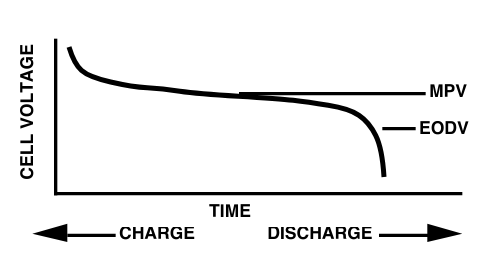
\includegraphics[width=0.6\textwidth]{img/chargeDischargeCurve_TxInst.png}
			\caption{Curva de la carga/descarga de una batería [\ref{bib: TI rechargeable batteries}].}
		\end{center}
	\end{figure}


	% \noindent Entrarían dentro de esta categoría  las conocidas baterías recargables, formato LiPo o Li-ion, por ejemplo, o formato powerbank, que si bien en su interior usan baterías LiPo/Li-ion, el encapsulado en el que se presentan y la forma en que se usan son totalmente diferentes. \\
	
	\noindent \textit{Tipos de baterías recargables}\\
	
	\noindent Las principales baterías recargables [\ref{bib: Hackaday battery basics}][\ref{bib: YouTube How to choose  a battery}][\ref{bib: blog diferencias li-ion y li-po}] que existen son: \\
	
	\begin{enumerate}
		
		\item \textit{Lithium polymer} (LiPo).  Son baterías de gran densidad de energía disponible, es decir, almacenan una gran cantidad de energía en comparación con el tamaño de la pila (se explica en \textit{Términos y definiciones}). Es por esta razón por la que los teléfonos móviles, los portátiles y otros dispositivos ligeros en peso usan baterías LiPo. Sin embargo, esta alta densidad de energía lleva consigo un coste/inconveniente, y es que son caras, y no son sólo las baterías en sí; cuando se trabaja con baterías de litio, hay que realizar una inversión para conseguir una circuitería especial que mantenga segura la batería. Por ejemplo, cuando estas cargando una batería LiPo, hay que asegurarse de que nunca se excedan los 4.2V por celda; las baterías LiPo explotarían si las sobrecargaras. No solo la carga de la batería es delicada, sino que la descarga también lo es; si se descarga una batería LiPo por debajo de 3V por celda, se perderá permanentemente parte de su capacidad, e incluso pueden deformarse/hincharse. Finalmente, hay que estar pendiente constantemente de la temperatura, para evitar que la batería se sobrecaliente. A pesar de todo esto, es común usar baterías LiPo en proyectos ligeros y pequeños, siempre y cuando se tenga un buen circuito de carga, un buen circuito de descarga (que proteja a valores bajos de tensión, haciendo de corte en el mínimo de tensión de la batería) y un buen circuito de monitorización de temperatura. 
		
		\item \textit{Lithium-ion} (Li-ion). Son muy similares a las baterías LiPo, pero a diferencia de estas, el electrodo negativo es líquido y el encapsulado y formato de presentación es totalmente diferente (las Li-ion suelen venderse sin protección y en apariencia son similares a unas pilas alcalinas AA). Una batería Li-ion almacena más potencia que las LiPo (mayor capacidad), ofrece mayores corrientes de descarga, es menos costosa de fabricar (y por tanto tienen un precio de venta más asequible),  y tiene un tiempo de vida más largo (aunque con el tiempo pierde sus propiedades). Es, al igual que las LiPo, inflamable si se daña, se calienta en exceso o se sobrecarga. El empaquetado más común es el 18650, y en el mercado existen circuitos de protección varios para evitar la sobrecarga y la sobredescarga  para este encapsulado en concreto, por lo que es una opción barata y sencilla para conseguir un prototipado rápido y realizar pruebas del mismo, siempre y cuando el proyecto no exija mucha potencia; si el proyecto exigiera más tensión de la que proporciona la batería, se puede considerar obtener más unidades y realizar una configuración en serie para aumentar la tensión, o en paralelo si lo que se desea es aumentar la capacidad, o una combinación de ambas configuraciones (usando siempre un \textit{Battery Management System} o BMS, para mantener las baterías balanceadas entre sí). Esta opción se puede considerar para baterías LiPo, pero para usuarios principiantes o poco experimentados resultará, probablemente, más complejo.
		
		\item \textit{Lithium Iron Phosphate} (LiFePO4). Son similares a las baterías LiPo, con la salvedad de que no son propensas a explosiones, como lo pueden ser las LiPo, si no se manipulan correctamente o las condiciones anteriormente mencionadas no se dan. También requieren una apropiada circuitería para cargarlas y descargarlas con cuidado, y si se comete un error se perderá permanentemente parte de la capacidad de la batería. Además, son un poco más pesadas que las baterías LiPo. Se usan normalmente en robots ligeros, herramientas eléctricas y juguetes por radio control, ya que son baterías bastante buenas entregando grandes cantidades de energía en un formato pequeño y liviano.
		
		\item \textit{Sealed lead-acid} (SLA). Son una opción si se quiere comprar una batería no muy costosa, a la vez de evitar enfrentarnos a circuitos de protección de la batería. Estas baterías son bastante más duraderas que una batería de litio, y también son mejores para hacer frente a sobrecargas accidentales o sobredescargas. Tienen una excelente relación calidad-precio y también son el mejor tipo de batería frente a temperaturas extremas; es por esta razón que las baterías de plomo (o ácido-plomo) son la opción estándar para coches, motos, almacenamiento de energía solar y fuentes de alimentación de emergencia. El inconveniente de usar baterías de plomo es que son grandes y pesadas. No es recomendable, por tanto, usar baterías de plomo en aplicaciones portátiles.
		
		\item Níquel-cadmio (\textit{Nickel-cadmium}, NiCd). Los dispositivos portátiles, como los primeros teléfonos móviles, usaban baterías de níquel-cadmio. Son baterías baratas, que en teoría duran más tiempo que las baterías SLA; sin embargo, sufren el llamado efecto memoria, por lo que hay que regularmente descargarlas por completo, luego recargarlas por completo para mantener una alta capacidad, ya que, de lo contrario, estaríamos perdiendo vida útil de la batería. Así pues, en la actualidad no se suele usar este tipo de baterías, aunque se siguen vendiendo.
		
		\item \textit{Nickel Metal Hydride} (NiMH). Las baterías de níquel-metalhidruro o de níquel hidruro metálico tienen una mayor densidad de energía que las baterías de níquel-cadmio, en tanto a precio no son mucho más costosas y no sufren el efecto memoria. Son más grandes y pesadas que las baterías de litio, pero es bastante seguro trabajar con ellas, por lo que son las baterías más usadas por el consumidor medio en términos de pilas recargables (las encontramos en cualquier supermercado, y cargarlas es barato y simple). Hay que tener en cuenta que las baterías de NiMH, por norma general, tienen un ratio de autodescarga elevado, lo que quiere decir que a pesar de que no se esté haciendo uso de la batería, se autodescargan igualmente en un par de meses, lo que hace que no sean una buena opción para objetos de uso cotidiano (como mandos a distancia). Se recomienda que, si se necesita hacer uso de este tipo de baterías, se adquieran con bajo ratio de autodescarga (como Panasonic Eneloop), las cuales pueden resultar más baratas a largo plazo que comprar unas pilas alcalinas.
		
	\end{enumerate}
	
	\noindent \textit{Comparativa entre tipos de baterías recargables} \\
	
	\noindent \textit{\textbf{Densidad de energía}}
	
		\begin{figure}[h]
		\begin{center}
			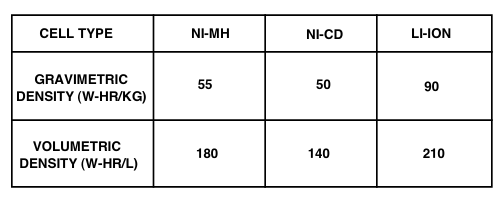
\includegraphics[width=0.7\textwidth]{img/energyDensityComparison_TxInst.png}
			\caption{Comparación densidad de energía para diferentes baterías [\ref{bib: TI rechargeable batteries}].}
			\label{fig: comparación densidad energía}
		\end{center}
	\end{figure}
	
	 
	
	\noindent Al revisar los datos de la Figura \ref{fig: comparación densidad energía}, la ventaja de Li-Ion en densidad gravimétrica es claramente la más sorprendente, casi duplicando las cifras de Ni-Cd y Ni-MH. Esto significa que los productos que funcionan con celdas de iones de litio se pueden hacer mucho más livianos sin sacrificar el tiempo de ejecución. Alternativamente, si el peso de la batería se mantiene igual, el tiempo de funcionamiento se duplicará si se utilizan baterías de iones de litio. Este hecho explica la razón por la que Li-Ion está reemplazando rápidamente al Ni-MH en los teléfonos celulares y computadoras portátiles de primera línea. \\
	
	\noindent \textit{\textbf{Estabilidad de tensión o tensión de celda}}\\
	
	\noindent La tensión proporcionada para alimentar la carga es la más importante: las baterías Ni-Cd y Ni-MH tienen una tensión por celda de 1.25V (sus tensiones de descarga se asumen por norma general idénticas). \\
	\noindent La tensión por celda de las baterías Ni-Cd y Ni-MH son sólo una tercera parte de la tensión nominal de 3.6V proporcionada por una celda de Li-ion (Figura \ref{fig: curva descarga celdas}), lo que significa que se requerirían tres celdas de Ni-Cd/Ni-MH conectadas en serie para igualar la tensión de una única celda de Li-ion.\\
	\noindent Sin embargo, la Figura \ref{fig: curva descarga celdas} muestra también la gran ventaja de las baterías Ni-Cd y Ni-MH: su curva de descarga es extremadamente plana, próxima a la de una batería ideal. Esta importante diferencia entre tipos de baterias significa que las celdas de Ni-Cd y Ni-MH son adecuadas para su uso con reguladores lineales, pero las baterías de Li-ion requieren convertidores reductores (\textit{Buck converters}) para obtener una buena eficiencia de conversión de energía en la fuente de alimentación. \\
		
	\begin{figure}[h]
		\begin{center}
			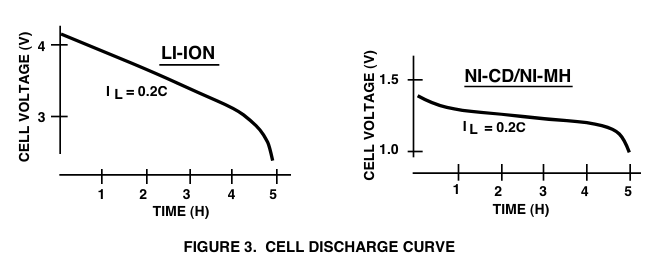
\includegraphics[width=0.7\textwidth]{img/cellDischargeCurve_TxInst.png}
			\caption{Curva de descarga de una celda Li-ion y una celda Ni-Cd/Ni-MH (caída de tensión conforme aumentan las horas de uso de la batería) [\ref{bib: TI rechargeable batteries}].}
			\label{fig: curva descarga celdas}
		\end{center}
	\end{figure}
	
	\pagebreak 
	
	\noindent \textit{\textbf{Corriente pico}}\\	
	
	\noindent \textit{\textbf{Autodescarga}}\\	
	
	\noindent \textit{\textbf{Tiempo de carga}}\\	
	
	\noindent \textit{\textbf{Coste}}\\
	
	\noindent \textit{\textbf{Fiabilidad}}\\		
	
	\noindent \textit{\textbf{Modos de falla relacionados con la edad}}\\	
	
	\noindent \textit{\textbf{Temperatura de funcionamiento}}\\	
	
	\noindent \textbf{Panel solar}\\ 
	
	\noindent Un panel solar, por si solo, no realiza la tarea de alimentación autónoma. Requiere, como mínimo, de una batería donde almacenar la energía que captan, por lo que, necesariamente, habría que escoger entre algunas de las opciones planteadas en el apartado anterior. Además, una batería no irá conectada directamente al panel solar, ya que se requiere un cargador solar que haga de intermediario, por una parte, entre la batería y el panel, y por otra parte, entre la batería y el dispositivo al que alimenta dicha batería. \\
	
	\noindent Aunque esto será explicado con más detalle más adelante, se considera necesario establecer desde un principio los requerimientos mínimos para poder usar un panel solar de cara a la funcionalidad de alimentación autónoma, ya que dependen del apartado que acabamos de presentar sobre baterías recargables, y estos requerimientos mínimos establecerán una base de cara a la explicación sobre sistemas fotovoltaicos más complejos. \\
	
	\noindent \textit{Funcionamiento y composición de un panel solar}
	
	\begin{figure}[h]
		\begin{center}
			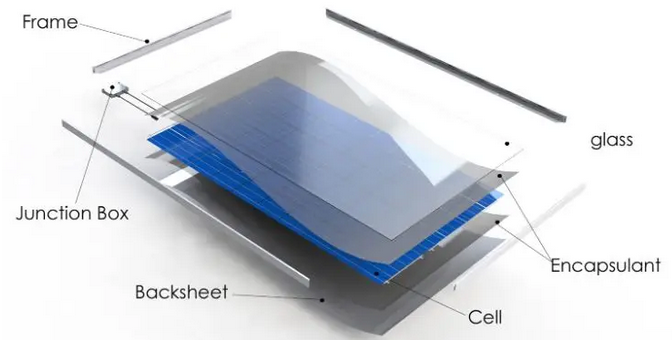
\includegraphics[width=0.6\textwidth]{img/layersSolarPanel.png}
			\caption{Capas y componentes que componen un panel solar [\ref{bib: solar reviews how solar panels work}].}
			\label{fig: capas panel solar}
		\end{center}
	\end{figure}

	\pagebreak
	
	\noindent Un panel solar es una agrupación de muchas células fotovoltaicas (PV) que están cubiertas con vidrio protector y unidas con un marco de metal. Es por eso que el nombre oficial de un panel solar es "módulo fotovoltaico" (\textit{PV module}). Estas células solares fotovoltaicas están hechas de material semiconductor, generalmente silicio, que se corta en tiras muy finas.\\
	
	\noindent Los paneles solares tienen muchas capas. La capa de células fotovoltaicas es donde se produce la electricidad. Otras capas, como las capas de vidrio y encapsulante, están ahí para proteger las células fotovoltaicas para que los módulos puedan producir electricidad de manera adecuada.\\
	
	\noindent Cada célula fotovoltaica tiene una capa negativa y una capa positiva. Para que un panel solar genere electricidad solo necesitamos algo de energía para hacer que esos electrones fluyan de la capa negativa a la capa positiva. \\
	
	\noindent Así pues, en resumen, la energía de los fotones del sol hace que los electrones en el lado negativo de la celda fotovoltaica se muevan (existe electricidad). Esto se llama \texttt{efecto fotovoltaico}.\\
	
	\begin{figure}[h]
		\begin{center}
			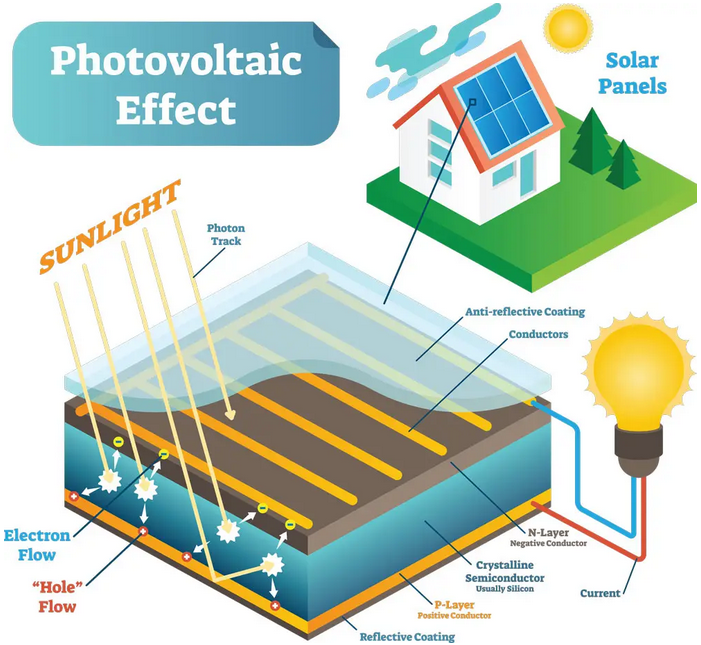
\includegraphics[width=0.6\textwidth]{img/photovoltaic_effect.png}
			\caption{Dibujo representativo del efecto fotovoltaico [\ref{bib: solar reviews how solar panels work}].}
			\label{fig: efecto fotovoltaico}
		\end{center}
	\end{figure}
	
	\pagebreak
	
	\noindent Los electrones necesitan un camino a seguir y la electricidad debe estar en una forma útil. Es por ello que la ruta que creemos para los electrones (el circuito) es importante, ya que, cuando salen de la capa negativa de la celda fotovoltaica, queremos que fluyan a través de nuestras cargas (como nuestras luces y electrodomésticos, en el ejemplo del uso doméstico) para que los electrones puedan dar energía a esas cargas a medida que avanzan hacia la capa positiva de la celda fotovoltaica. \\
	
	%\noindent \textit{¿explicación sistema fotovoltaico?} \\
	
	\noindent Un elemento muy importante en este sentido es el inversor, el cual convierte la energía DC producida por un panel solar, a energía AC, lista para ser usada en el hogar. Sin embargo, para nuestro proyecto no es necesario, ya que nos interesa crear un proyecto que se alimente de manera autónoma, sin uso de la electricidad disponible en el hogar; el panel solar, en este caso, recargaría una pila, y por ello necesitamos la energía DC, y no necesitamos usar un inversor a AC. \\ 
	
	\noindent \textit{Parámetros}\\
	
	\noindent Los principales paramétros que se usan para caracterizar el rendimiento de las células solares son la potencia máxima $P_{max}$ (\textit{peak power}), la densidad de corriente en cortocircuito $J_{sc}$, la tensión en circuito abierto $V_{oc}$, y el factor de forma \textit{FF}. Estos parámetros se determinan a partir de la curva J-V característica cuando la célula está iluminada, tal como se muestra en la Figura \ref{fig: curva J-V célula solar}. La eficiencia de conversión $\eta$ se puede determinar a partir de estos parámetros. \\
	
	\noindent Nótese que se menciona específicamente \textit{parámetros de una célula solar}; un panel solar, como se ha mencionado anteriormente, consta de varias células fotovoltaicas, por lo que los parámetros especificados, en términos globales y tal como se construyen los paneles solares, influyen en las especificaciones finales del panel según el número de células del que conste (ver Figura \ref{fig: solar panel of identical solar cells}). \\
		\begin{figure}[h]
		\begin{subfigure}{0.5\textwidth}
			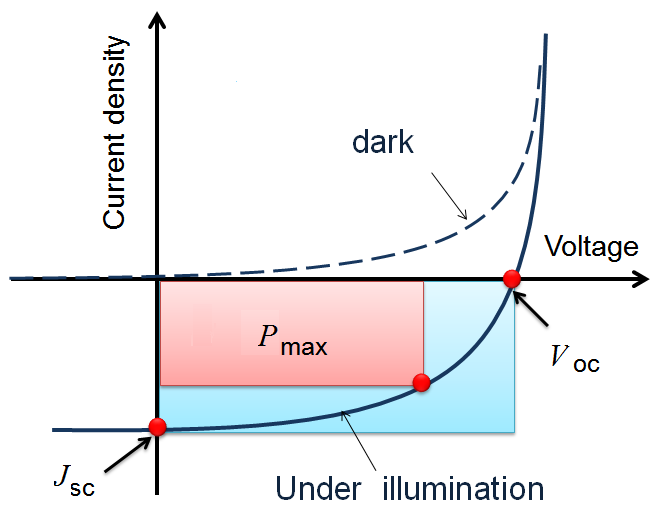
\includegraphics[width=1\textwidth]{img/JV_curve_solarCell.png} 
			\caption{Determinación de los parámetros de una célula solar a partir de su curva J-V [\ref{bib: research gate JV curve solar panel}].}
			\label{fig: curva J-V célula solar}
		\end{subfigure}
		\begin{subfigure}{0.5\textwidth}
			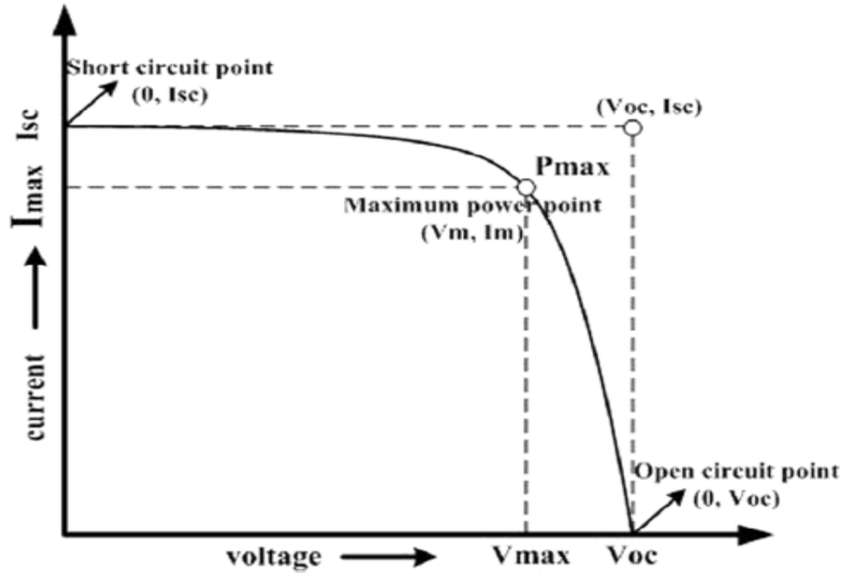
\includegraphics[width=1\linewidth]{img/IV_curve_solarCell.png}
			\caption{Curva I-V de una célula solar [\ref{bib: research gate pv cell param}].}
			\label{fig: I-V curve of a solar cell}
		\end{subfigure}
		\caption{Curvas J-V e I-V de una célula fotovoltaica}
		\label{fig:curvas J-V e I-V célula PV}
	\end{figure}

	\begin{figure}[h]
		\begin{center}
			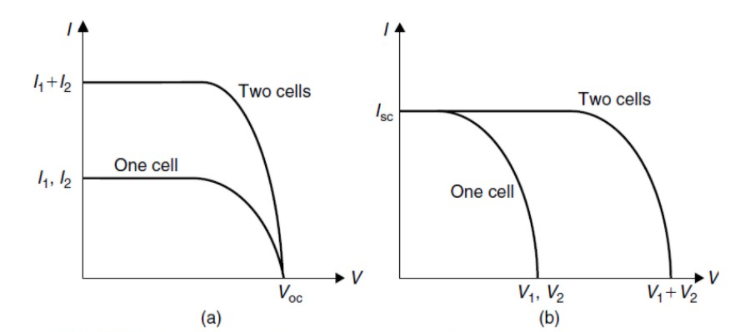
\includegraphics[width=0.7\textwidth]{img/effectTwoIdenticalCells.png}
			\caption{Comportamiento de un panel solar formado por dos células solares idénticas [\ref{bib: SlidePlayer Photovoltaic systems}].}
			\label{fig: solar panel of identical solar cells}
		\end{center}
	\end{figure}
	

	\noindent Para realizar medidas fiables y definir la curva característica J-V, se deben realizar las medidas bajo condiciones estándar de pruebas (\textit{standard test conditions, STC}); estas son, una temperatura constante a $25^{\circ}C$, una irradiancia total de 1000 $W/ m^2$ y un espectro solar de AM1.5 (sol directo y con ángulo cenital de $48,2 ^{\circ}$). Esto lo tendremos en cuenta si queremos comprobar que las especificaciones del producto son correctas, o por el contrario el producto viene tiene defectos. En este proyecto no es prioritario el estudio profundo y comprobación exhaustiva del panel solar, por lo que no se realizarán dichas pruebas; sin embargo, sí realizaremos un estudio teórico de los parámetros que definen a una célula solar, como también lo hemos hecho de los materiales que lo componen y su funcionamiento general.\\
	
	
	\noindent \textit{\textbf{Densidad de corriente en cortocircuito}} \\
	
	\noindent La corriente en cortocircuito $I_{sc}$ es la corriente que fluye a través de un circuito externo cuando los electrodos de una célula solar se cortocircuitan. La corriente en cortocircuito de una célula solar depende de la incidencia del flujo de fotones sobre ella, la cual está determinada por el espectro de la luz incidente. También depende del área de la célula solar. Para eliminar la dependencia del área de la célula solar sobre $I_{sc}$, normalmente se usa la densidad de corriente en cortocircuito para describir la máxima corriente entregada por una célula solar. La máxima corriente que una célula solar puede entregar depende mucho de las propiedades ópticas de la célula solar, tales como la absorción en la capa absorbente y la reflexión. \\
	
	\noindent Las células solares de silicio cristalino pueden entregar, bajo un espectro AM1.5, una posible densidad de corriente máxima de 46 $mA/cm^2$. En las células solares de c-Si de laboratorio, las medidas de $J_{sc}$ están por encima de 42 $mA/cm^2$, mientras que las células solares comerciales tienen un $J_{sc}$ que excede los 35 $mA/cm^2$. \\
	
	\noindent \textit{\textbf{Tensión en circuito abierto, $V_{oc}$}} \\
	
	\noindent Es la tensión máxima que una célula solar puede entregar. $V_{oc}$ corresponde a la tensión de polarización directa, a la cual la densidad de corriente de oscuridad compensa la densidad de corriente fotovoltaica (\textit{fotocorriente}). Depende de la densidad de corriente de saturación de la célula solar y de la corriente fotogenerada. Mientras ésta última varía poco, la corriente de saturación puede variar en órdenes de magnitud. La corriente de saturación depende de la recombinación en la célula solar, por lo que $V_{oc}$ es una medida de la cantidad de recombinación de la célula solar.\\
	
	\noindent Las células solares de laboratorio hechas de silicio cristalino dan valores de $V_{oc}$ de hasta 720 mV bajo condiciones AM1.5 estándar, mientras que las células solares comerciales normalmente dan valores de $V_{oc}$ por encima de los 600 mV. \\
	
	\noindent \textit{\textbf{Factor de forma}} \\
	
	\noindent El factor de forma es la relación entre la potencia máxima ($P_{max} = J_{mpp} V_{mpp}$) generada por una célula solar y el producto de $V_{oc}$ con $J_{sc}$. \\
	
	\noindent El subíndice \textit{mpp} hace referencia al \textit{punto de potencia máxima} (\textit{maximum power point, MPP}) de la célula solar, es decir, el punto de la curva característica J-V de la célula solar al cual la célula solar ofrece su máxima potencia de salida.  Para optimizar la operación de los sistemas fotovoltaicos, es muy importante que las células solares (o módulos fotovoltaicos) operen sobre el MPP. Esto se puede asegurar con un seguidor de punto de máxima potencia (\textit{maximum power point tracking, MPPT}). Se trata de un algoritmo, el cual se usa en controladores de carga solar para extraer la máxima potencia disponible del módulo fotovoltaico bajo ciertas condiciones; dichas condiciones (se entrará más en detalle más adelante), como son la radiación solar a lo largo del día y año, la temperatura ambiente y la temperatura de la célula, afectan a la potencia máxima de salida de la misma, y es entonces cuando un MPPT actúa, haciendo operar a la célula solar al valor de tensión más eficiente, el MPP. El controlador de carga mantiene la tensión y la corriente a un nivel optimizado, donde el módulo fotovoltaico brinda la mayor cantidad de energía a la carga; es ``consciente'' del estado de carga de la batería y actúa en consecuencia. \\
	
	\noindent El uso de un seguidor de punto de máxima potencia, sin embargo, encarece el costo total de un proyecto; si bien para aplicaciones que requieran la extracción de la máxima potencia de un panel solar (por limitaciones de espacio, por ejemplo, donde deberíamos explotar las características de los paneles que pudiéramos colocar), en el proyecto que estamos diseñando no es el caso, por lo que no usaremos herramientas de este estilo. Además, aunque pueden encontrarse o construirse de manera aislada (se trata de un conversor DC a DC), también suelen encontrarse incorporados a inversores, los cuales tampoco son necesarios, ya que no es energía solar para uso en hogar. Como anotación, existen otros controladores de carga que no son MPPT, como el PWM o \textit{shunt controller} (regulador de carga tipo paralelo o de desviación). \\
	
	\begin{figure}[h]
		\begin{center}
			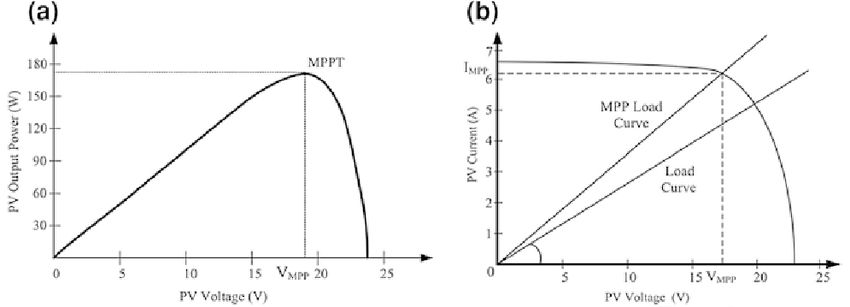
\includegraphics[width=0.7\textwidth]{img/mppt_curve.png}
			\caption{Curva P-V de una célula solar, indicando el punto MPP [\ref{bib: research gate mppt curve}].}
			\label{fig: MPPT in P-V curve of a solar cell}
		\end{center}
	\end{figure}
	
	\noindent Por último, anotar que el factor de forma no varía tanto con $V_{oc}$, sino más con el material del que están hechas las células solares. \\
	

	\noindent \textit{\textbf{Eficiencia de conversión}} \\
	
	\noindent La eficiencia de conversión se calcula como la relación entre la potencia potencia generada y la potencia incidente.  Como vemos en la siguiente fórmula, y tal como establece su propia definición, depende de todos los parámetros anteriormente descritos: \\
	
	\begin{equation}
		 \eta = \frac{P_{max}}{I_{in}} = \frac{J_{mpp} V_{mpp}}{I_{in}} = \frac{J_{sc} V_{oc} FF}{I_{in}} 
	\end{equation}
	
	\noindent Los parámetros externos típicos de una célula fotovoltaica de silicio cristalino son $J_{sc} \approx 35 mA/cm^2$, $V_{oc}$ hasta 0.65V y FF en el rango entre 0.75 y 0.80; esto implica que la eficiencia de conversión caiga en el rango entre 17 y 18 \%. \\
	
	\noindent \textit{\textbf{Circuito equivalente}} \\
	
	\noindent Una célula fotovoltaica iluminada puede comportarse como un diodo ideal, y este comportamiento puede describirse a través de un circuito equivalente simple, como el que se muestra en la Figura \ref{fig: equivalent circuit solar cell} (a). donde un diodo y una fuente de corriente están conectados en paralelo. El diodo está formado por una unión p-n. \\
	
	\begin{figure}[h]
		\begin{center}
			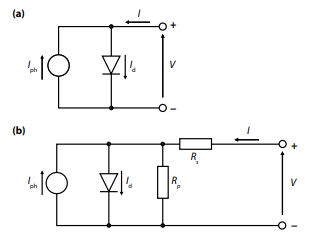
\includegraphics[width=0.5\textwidth]{img/circuitEquivalent_solarCell.png}
			\caption{Circuito equivalente de una célula fotovoltaica, en el caso ideal (a) y considerando pérdidas (b) [\ref{bib: TU delft OCW solar cell param}].}
			\label{fig: equivalent circuit solar cell}
		\end{center}
	\end{figure}
	
	\pagebreak
	
	\begin{figure}[h]
		\begin{center}
			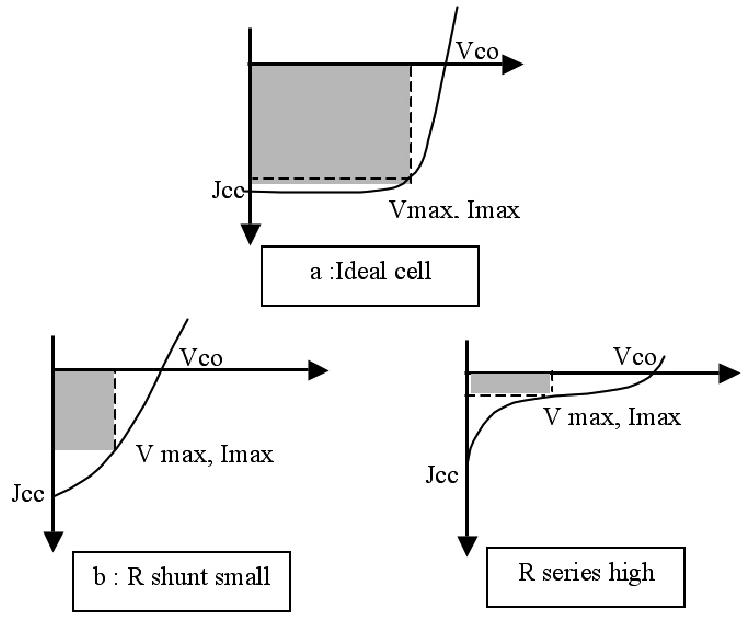
\includegraphics[width=0.6\textwidth]{img/JV_curve_withRsRp.png}
			\caption{Curva J-V de una célula fotovoltaica, mostrando el efecto de aumentar o disminuir el valor de las resistencias $R_{s}$ y $R_{p}$ o $R_{sh}$ (\textit{shunt}) [\ref{bib: SciELO}].}
			\label{fig: JV curve with non-ideal model (one diode)}
		\end{center}
	\end{figure}

	\noindent Sin embargo, en la práctica, el factor de forma está influenciado por una resistencia en serie $R_{s}$, y una resistencia de derivación $R_{p}$. La influencia de estos parámetros en la curva característica J-V de una célula solar puede estudiarse usando el circuito equivalente mostrado en la Figura \ref{fig: equivalent circuit solar cell} (b). Además, en células solares reales, el factor de forma también está influenciado por una recombinación adicional que ocurre en la unión p-n. Este diodo no ideal se representa normalmente con un circuito equivalente formado por dos diodos, uno ideal con un factor de idealidad\footnotemark \enspace igual a la unidad, y otro diodo no ideal con un factor de idealidad mayor que uno. \\
	
	\footnotetext{El factor de idealidad del diodo es una medida de cómo de cerca el diodo sigue la ecuación del diodo ideal.}

	
	\begin{figure}[h]
		\begin{center}
			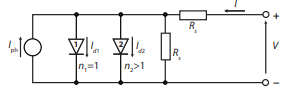
\includegraphics[width=0.5\textwidth]{img/nonIdeal_equivCircuit_solarCell.png}
			\caption{Circuito equivalente de una célula fotovoltaica con un modelo de dos diodos, donde $n_{1}$ y $n_{2}$ son los factores de idealidad e $I_{d1}$ y $I_{d2}$ las corrientes que atraviesan cada diodo [\ref{bib: TU delft OCW solar cell param}].}
			\label{fig: non-Ideal equivalent circuit solar cell}
		\end{center}
	\end{figure}	
	
%	\noindent Uno de los parámetros más importantes en un panel solar es la \texttt{eficiencia}. Mide el porcentaje de luz solar que llega a la celda solar y que se convierte en electricidad utilizable. Cuanto mayor sea la eficiencia, menor será la superficie que necesitarán los paneles solares para satisfacer sus necesidades energéticas, pero mayor será el precio. \\
	
%	\noindent Algunas personas asocian mayores niveles de eficiencia con paneles de mayor calidad, pero esto no es necesariamente cierto. Alta eficiencia significa que su sistema fotovoltaico solar utilizará menos espacio en su azotea. Por lo tanto, quienes viven en áreas de alta densidad y tienen un espacio muy limitado para la energía solar generalmente están más preocupados por los niveles de eficiencia. \\
	
	\noindent \textit{Factores principales que influyen en la potencia de salida de una célula PV}\\
	
	\noindent \textit{\textbf{Radiación solar}}
	\begin{figure}[h]
		\begin{subfigure}{0.45\textwidth}
			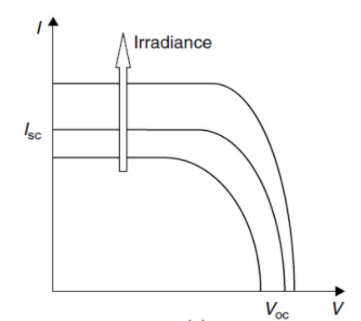
\includegraphics[width=0.8\textwidth]{img/generalEffect_irradianceIVcurve_solarCell.png} 
			\caption{Efecto general [\ref{bib: SlidePlayer Photovoltaic systems}].}
			\label{fig: variación general en la curva I-V de una célula PV con la intensidad de la radiación solar.}
		\end{subfigure}
		\begin{subfigure}{0.5\textwidth}
			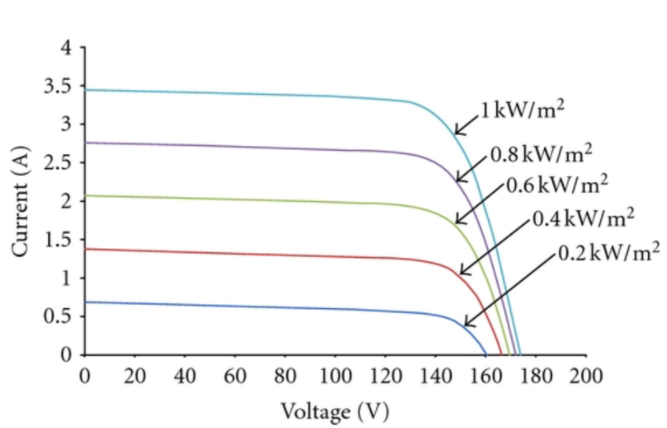
\includegraphics[width=1.05\linewidth]{img/concreteEffect_irradianceIVcurve_solarCell.png}
			\caption{Efecto según valores concretos de radiación [\ref{bib: research gate pv power}].}
			\label{fig:variación con valores en la curva I-V de una célula PV con la intensidad de la radiación solar.}
		\end{subfigure}
		\caption{Variación en la curva I-V ante la radiación solar.}
		\label{fig:variación I-V radiación solar}
	\end{figure}
	
	\pagebreak
	
	\noindent \textit{\textbf{Temperatura ambiente y temperatura de la célula}} \\
	
	\begin{figure}[h]
		\begin{subfigure}{0.45\textwidth}
			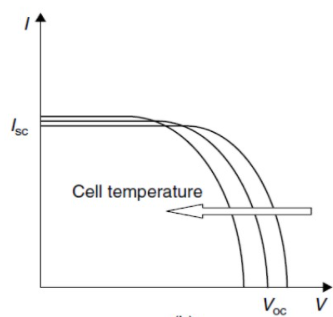
\includegraphics[width=0.8\textwidth]{img/generalEffect_celTempIVcurve_solarCell.png} 
			\caption{Efecto general [\ref{bib: SlidePlayer Photovoltaic systems}].}
			\label{fig: variación general en la curva I-V de una célula PV con la temperatura.}
		\end{subfigure}
		\begin{subfigure}{0.55\textwidth}
			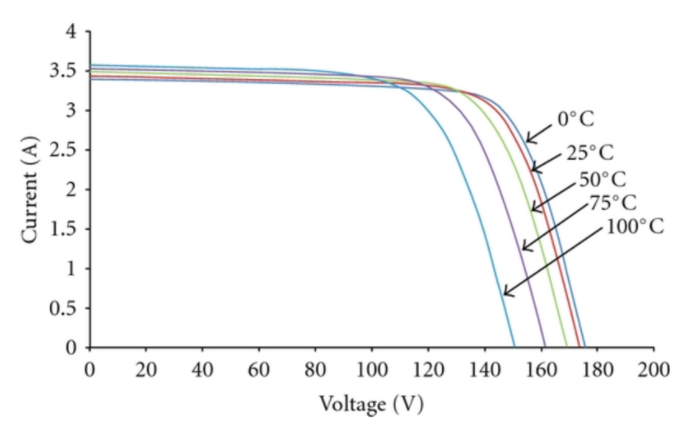
\includegraphics[width=1\linewidth]{img/concreteEffect_TempIVcurve_solarCell.png}
			\caption{Efecto según valores concretos de temperatura ambiente [\ref{bib: research gate pv power}].}
			\label{fig:variación con valores en la curva I-V de una célula PV con la temperatura.}
		\end{subfigure}
		\caption{Variación en la curva I-V ante la temperatura ambiente}
		\label{fig:variación I-V temperatura}
	\end{figure}
	
	\noindent Nótese que en la Figura \ref{fig: variación general en la curva I-V de una célula PV con la temperatura.} se hace referencia a \textit{temperatura de la célula} y en la Figura \ref{fig:variación con valores en la curva I-V de una célula PV con la temperatura.} a \textit{temperatura ambiente}. Si bien son dos magnitudes diferentes, la temperatura ambiente tiene un efecto sobre la temperatura de la célula que puede considerarse lineal. A una temperatura ambiente de $25^{\circ}C$, la temperatura de una célula de silicio cristalino suele situarse en el valor de $48^{\circ}C$. \\
	
	\begin{figure}[h]
		\begin{subfigure}{0.52\textwidth}
			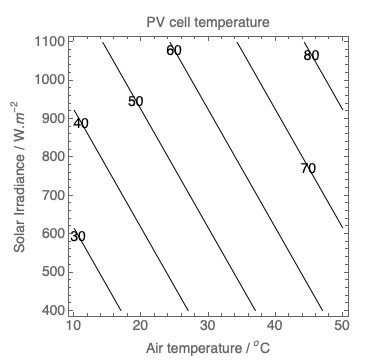
\includegraphics[width=1\textwidth]{img/PVcellTemp_AirTemp.png} 
			\caption{}
			\label{fig: solar cell temp vs air temp.}
		\end{subfigure}
		\begin{subfigure}{0.55\textwidth}
			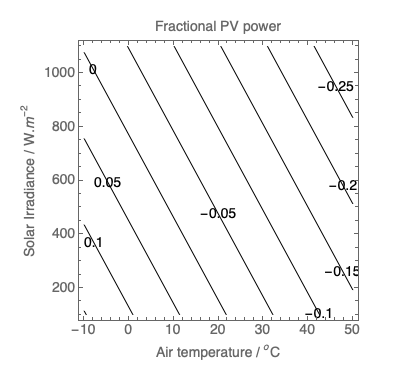
\includegraphics[width=1\linewidth]{img/powerPVCell_airTemp.png}
			\caption{}
			\label{fig:power output of a solar cell vs air temp.}
		\end{subfigure}
		\caption{Relación entre temperatura ambiente, radiación solar, con la potencia de salida de una célula PV (\ref{fig: solar cell temp vs air temp.}) y temperatura de ésta (\ref{fig:power output of a solar cell vs air temp.}) [\ref{bib: QVP air temp affect solar panel output}].}
		\label{fig:solar temp}
	\end{figure}
	
	\pagebreak
	
	%\noindent \href{https://www.qpvgroup.org/blog/2019/2/3/how-does-air-temperature-affect-photovoltaic-solar-panel-output}{LEER ESTO Y COMENTAR POR AQUÍ, inclusive fórmula porque es relación lineal entre temperaturas ambiente y célula} \\
	
	\begin{figure}[h]
		\begin{center}
			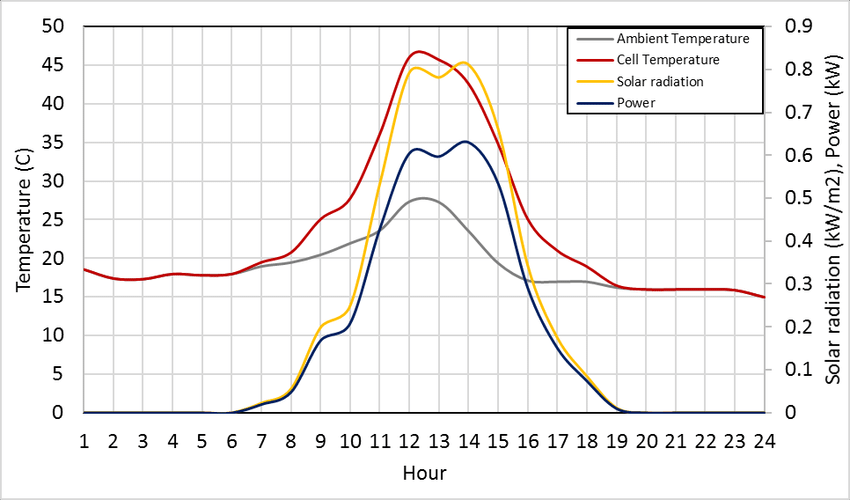
\includegraphics[width=0.7\textwidth]{img/cellTemp_ambTemp_Irrad_Pow.png}
			\caption{Variación de la potencia de salida de una célula PV dependiendo de la hora del día, la temperatura y la radiación solar [\ref{bib: research gate pv cell temp vs others}].}
			\label{fig:cellTemp_ambTemp_Irrad_Pow}
		\end{center}
	\end{figure}
	
	\pagebreak
	
	\noindent \textit{Opciones: tipos de paneles solares}\\
	
	\noindent Existen diferentes tipos de células fotovoltaicas disponibles en el mercado, aunque en su mayoría están fabricadas de silicio (Si), el segundo elemento más abundante en la corteza terrestre (después del oxígeno), el cual es el mismo material del cual está hecha la arena. El silicio por sí mismo no es muy puro y debe ser refinado para conseguir una pureza de hasta el 99.99 \% antes de que pueda usarse como material semiconductor en muchos tipos distintos de células fotovoltaicas, transistores o circuitos integrados digitales. El uso de silicio en la fabricación de células fotovoltaicas produce la típica célula fotovoltaica de color azul uniforme. \\
	\noindent Los dos tipos principales de materiales usados para células fotovoltaicas son el silicio cristalino y los depósitos de película fina, los cuales varían entre unos y otros en términos de eficiencia en absorción de luz, eficiencia en la conversión de energía, tecnología de fabricación y coste de producción. Las células fotovoltaicas (a partir de ahora, células PV, \textit{PhotoVoltaic}) hechas de silicio cristalino son el tipo más común de células PV que se utilizan en la actualidad y también son uno de los primeros dispositivos PV que tuvieron éxito.\\
	
	\noindent Los tres tipos generales de células PV hechas de silicio son:\\ 
	
	\begin{itemize}
		\item Silicio monocristalino, conocido tambien como silicio de un único cristal, cristal de silicio único o silicio monocristal (\textit{Mono-crystalline silicon, single-crystal silicon}).
		\item Silicio policristalino, conocido tambien como silicio de varios cristales, silicio multicristalino o silicio multicristal (\textit{Poly-crystalline silicon, multi-crystal silicon}).
		\item Silicio de película fina. \\
	\end{itemize}

	\noindent \textit{\textbf{Silicio cristalino (c-Si)}} \\
	
	\noindent \textit{\textbf{Célula PV de película fina}} \\
	
	\noindent \textit{\textbf{Otros tipos de células PV}} \\
	
	\subsubsection{Automatización y monitorización}
	\label{subsección 3.2.2: automatización y monitorización}
	
	\noindent En este apartado, se mostrará una visión de conjunto acerca de aquellos elementos mediante los cuales consigamos el objetivo de automatizar y monitorizar el sistema de alimentación. Se presentará el resultado de investigar sobre opciones que puedan ayudar a la consecución de los objetivos, tanto en la parte de microcontrolador como en la parte de comunicación radio, y demás actuadores y sensores en las partes de bebedero y comedero. Hay que tener presente que en todo momento se estarán buscando soluciones \textit{Open Source}, ya que se planteó como objetivo y filosofía a seguir en este proyecto.\\
	
	\subsubsubsection{Microcontrolador}
	
	\noindent \textit{Aclaración:} a lo largo de este apartado y consecutivos se hablará de la palabra microprocesador y microcontrolador. Se usará la palabra microcontrolador para determinar el conjunto global de una placa cuyo corazón sea un microcontrolador, de manera que podamos aligerar un poco la literatura y lectura de este documento. Un microprocesador es la CPU, mientras que un microcontrolador conforma un sistema embebido en un único \textit{chip} formado por memoria, procesador y entradas/salidas programables. Por ejemplo, llamaremos microcontrolador al arduino nano o uno porque se basa en el microcontrolador ATmega328.\\
	
	\noindent En tanto a microcontroladores, la opción \textit{Open Source} más conocida seguramente sea Arduino. Sin embargo, no significa que no existan más opciones en tanto a microcontroladores. Es importante recordar que ni Arduino ni las alternativas que se van a presentar son ordenadores, son microcontroladores, esto es, circuitos integrados diseñados para llevar a cabo una tarea única de manera cíclica (una vez que programado para una tarea, ejecutará esa tarea y sólo esa tarea una y otra vez, dependiendo de cómo haya sido programado).\\
	
	\noindent A continuación, se va a presentar una lista con algunas opciones de microcontroladores [\ref{bib: arduino alternatives}][\ref{bib: microcontrollers alternative to arduino}][\ref{bib: alternative to arduino}]. Vale la pena señalar que la mayoría de estas placas tienen variaciones que también vale la pena revisar; la elección de un microcontrolador u otro dependerá de lo que necesite nuestro proyecto (si necesita muchas entradas porque tendremos muchos periféricos, si necesitamos ahorro de energía al máximo, o una buena potencia de procesamiento, etc). \\
	
	\begin{itemize}
		\item \textbf{Arduino}. Se trata de una plataforma de desarrollo Open Source hardware y software, característica por su facilidad de uso e integración entre la solución hardware (placas Arduino) y la solución software (Arduino IDE). Existe una gama variada de placas Arduino, entre las que podemos destacar la nano o la uno. A modo de ejemplo, se mostrará la información de la uno, placa recomendada por la propia organización Arduino para principiantes.\\
		
		\textit{Especificaciones:} ATMega328P a 16 MHz, 32 kB de memoria flash, 2kB de SRAM y 1kB de EEPROM.\\
		
		\textit{Características:} 14 pines I/O digitales, 6 entradas analógicas, conexión USB, conector jack. \\
		
		\textit{Precio:} 20 \euro \enspace en Arduino.\\
		
		\item \textbf{NodeMCU}. NodeMCU (\textit{Node MicroController Unit}) es un entorno de desarrollo de software y hardware de código abierto que se basa en un sistema en chip (SoC) muy económico llamado ESP8266. El ESP8266, diseñado y fabricado por Espressif Systems, contiene todos los elementos cruciales de un ordenador: CPU, RAM, redes (wifi) e incluso un sistema operativo y SDK modernos. Cuando se compra por separado, el chip ESP8266 cuesta solo 2\$ por unidad. Esto lo convierte en una buena opción para proyectos de IoT de todo tipo. \\
		
		\textit{Especificaciones:} SoC basado en ESP8266 a 80 MHz, 64 kB de SRAM, 4 MB de memoria flash.\\ 
		
		\textit{Características:} compatibilidad con Arduino IDE, 16 GPIO, USB-TTL en CP2102 incluido onboard, tamaño reducido, puerto micro-USB, WiFi.\\
		
		\textit{Precio:} aprox. 8 \euro \enspace en Amazon.\\
	
		\item \textbf{STM32}. La familia STM32 de microcontroladores de 32 bits basada en el procesador Arm Cortex-M ofrece productos que combinan un rendimiento muy alto, capacidades en tiempo real, procesamiento de señales digitales, operación de bajo consumo / bajo voltaje y conectividad, mientras se mantiene una integración completa y facilidad de desarrollo.
		
		La gama de microcontroladores STM32, basada en un núcleo estándar de la industria, viene con una amplia variedad de herramientas y software para respaldar el desarrollo de proyectos, lo que hace que esta familia de productos sea ideal tanto para proyectos pequeños como para plataformas de extremo a extremo. \\
		
		\textit{Especificaciones:} depende del microcontrolador. Ejemplo de STM32F103C876, 72MHz Cortex-M3, SRAM de 20kB, 64/128 kB de memoria flash. \\
		
		\textit{Características:} software propio pero compatible con Arduino IDE, tamaño similar al arduino nano, dependiendo del microcontrolador tendremos diferentes tipos dentro de la gama STM32 (bajo consumo, altas prestaciones, conectividad, mainstream). \\
		
		\textit{Precio:} depende del microcontrolador. En este ejemplo, aprox. 10\$ en eBay. \\
		
		\item \textbf{The Pinguino 45K50}. Pinguino Project existe para acercar la simplicidad del lenguaje Arduino a los microcontroladores PIC de Microchip pero con un hardware USB incorporado y una placa que se puede construir en casa. El 45K50 es una de las opciones que nace de este proyecto Open Source.  Viene como un kit que se debe ensamblar antes de usarlo. \\
		
		\textit{Especificaciones:} procesador de 12 MIPS de 8 bits que se ejecuta a 48 MHz.\\
		
		\textit{Características:} 17 entradas / salidas digitales con 5 entradas analógicas compartidas, 2 salidas PWM, UART para comunicación en serie, etc.  IDE propio, también Open Source, compatible con el lenguaje Arduino y sus librerías.\\
		
		\textit{Precio:} aprox. 25\$.\\
		
		\item \textbf{Nanode}. Nanode ofrece una amplia gama de microcontroladores. Viene como un kit de desarrollo, lo que significa se debe ensamblar y soldar previamente antes de comenzar con la placa. 	El microcontrolador Nanode puede servir como alternativa a Arduino Uno, Mega y Yun, y también es Open Source.
		
		\textit{Especificaciones:} ATMega328P a 16MHz, 2kB de SRAM, 1kB de EEPROM, 32kB de memoria flash ISP.\\
		
		\textit{Características:} mini USB, controlador ethernet ENC8J60, conector ethernet, LEDs de diagnóstico.\\
		
		\textit{Precio:} aprox. 50\$.\\
		
		\item \textbf{Teensy 3.6. o Teensy 2.0}. La familia de placas Teensy fue desarrollada por PJRC durante los últimos años. Inicialmente, Teensy se creó prometiendo un poco más de factor de forma más pequeño. Uno de los Teensy más apreciados es el 3.6.; tiene un procesador ARM de 32 bits, 52 entradas/salidas en total, ADC, lector de tarjetas SD y muchas más funciones. Además, PJRC proporciona un complemento software \textit{Teensyduino} para una compatibilidad casi completa con los programas Arduino. \\ 
		
		\textit{Especificaciones}: 180-MHz Cortex M4F, 256 kB RAM, almacenamiento flash 1MB, 4K EEPROM. \\
		
		\textit{Características}: Teensyduino para Arduino IDE, lector SD. \\
		
		\textit{Precio}: aprox. 30 \$ en PJRC. \\
		
		\item \textbf{Launchpad MSP430}. Launchpad es una placa de desarrollo fabricada por Texas Instruments (TI). Junto con el hecho de que viene con un MSP430 de TI, también brinda compatibilidad con el software y hardware de TI. Esto viene en forma de paquetes de refuerzo y herramientas de desarrollo en línea. Además, permite la depuración onboard. Existe un IDE similar a Arduino llamado Energia para un enfoque más sencillo. \\
		
		\textit{Especificaciones}: 24-MHz MSP430, 32 kB Program FRAM, 4 kB RAM. \\
		
		\textit{Características}: tecnología \textit{EnergyTrace} para bajo consumo, Energia (similar a Arduino IDE), dos botones onboard y LEDs, compatible con el \textit{Booster Pack}. \\
		
		\textit{Precio}: aprox. 13 \$ en Texas Instruments. \\
		
		\item \textbf{Netduino N3 Wi-Fi}. Una alternativa diferente a Arduino de Wilderness Labs, el Netduino N3 utiliza .NET MicroFramework y Netduino.Foundation Framework, lo que significa que está programado en un lenguaje de programación de nivel superior (C\#). Esto puede resultar atractivo para aquellos que no quieren lidiar con los niveles más bajos de programación de MCU.
		
		Esta placa, con Wi-Fi incorporado, está diseñada para conexión inalámbrica entre dispositivos. Otra característica notable de Netduino es la disposición de los pines hecha para la compatibilidad del shield Arduino. Dicho todo esto, Netduino puede atraer a aquellos que ya están familiarizados con el marco .NET y les gustaría programar su placa MCU a través de Microsoft Visual Studio y similares. \\
		
		\textit{Especificaciones}: 168 MHz, 164+ kB RAM, 1408kB de almacenamiento flash.  \\
		
		\textit{Características}: .NET  MicroFramework, librerías Netduino.Foundation, Wi-Fi, lector SD,  22 pines de entrada-salida de propósito general (GPIO). \\
		
		\textit{Precio}: aprox. 50\$. \\
		
		\item \textbf{Particle Photon}. Particle Photon es la placa ideal para el proyecto de IoT conectado. El Photon tiene un chip Wi-Fi Cypress integrado y viene con conectividad gratuita con Device Cloud y todas sus funciones. Particle incluso proporciona JavaScript y SDK móviles junto con su IDE web y local.
		
		Gracias a todo el soporte, guías y herramientas proporcionadas por Particle, Photon es una buena alternativa a Arduino. Es ideal para aficionados principiantes o intermedios que buscan la plataforma adecuada para un proyecto de IoT simple. \\
		
		\textit{Especificaciones}:  ARM Cortex M3 de 120 MHz, RAM de 128 kB, almacenamiento flash de 1 MB.\\
		
		\textit{Características}: Device Cloud, SDK para dispositivos móviles y ParticleJS, 18 GPIO, muchas referencias y guías. \\
		
		\textit{Precio}: aprox. 19\$.\\
		
		\item \textbf{SparkFun Thing Plus}. SparkFun tomó el ESP32 e hizo esta placa. El ESP32 es sin duda una gran opción para una placa IoT. Viene con Wi-Fi, Bluetooth y Bluetooth Low Energy integrados. Incluso agregaron una conexión Li-Po para complementar aún más su naturaleza inalámbrica.
		
		Thing Plus también muestra algunas especificaciones impresionantes y un buen conjunto de sensores. Además, es compatible con Arduino IDE. \\
		
		\textit{Especificaciones}: 240 MHz, 520 kB SRAM, 16MB de almacenamiento flash. \\
		
		\textit{Características}: Wi-Fi, Bluetooth, BLE, cargador de batería Li-Po, sensor de efecto Hall, sensor táctil capacitivo, sensor de temperatura. \\
		
		\textit{Precio}: aprox. 21\$ en SparkFun.\\
		
		\item \textbf{Adafruit Feather Huzzah}. El Huzzah proviene de la línea Feather de Adafruit. Está destinado a ser una placa pequeña. Tiene Wi-Fi incorporado, un cargador Li-Po y compatibilidad con Arduino. Además, como ESP8266, se puede utilizar con NodeMCU Lua.
		
		Puede parecer que esta placa parece una versión inferior de Thing Plus, ya que el ESP32 es esencialmente el sucesor del ESP8266. Esta placa, sin embargo, ha existido lo suficiente como para que haya ganado una gran comunidad de usuarios. Esto hace que esta placa sea accesible para los aficionados que deseen la experiencia colectiva de dicha comunidad. \\
		
		\textit{Especificaciones}: 80 MHz, 50 kB RAM, 4MB de almacenamiento flash. \\
		
		\textit{Características}: Wi-Fi, cargador Li-Po, compatible con Arduino, NodeMCU Lua, 9 GPIO.\\
		
		\textit{Precio}: aprox. 17\$ en Adafruit.\\
		
		\item \textbf{BeagleBoard PocketBeagle}. El PocketBeagle es el más pequeño de los BeagleBoards. Ejecuta Linux desde el primer momento y se puede programar a través de su navegador web. Esta opción, por tanto, se trataría de un ordenador, como lo es una Raspberry Pi, no un microcontrolador. Ideal para proyectos pequeños que necesitan los recursos de una computadora. 
		
		El Sitara AM3358 ARM Cortex-A8 en el PocketBeagle tiene dos PRU (unidades programables en tiempo real) que son esencialmente microcontroladores conectados al procesador principal. Estos son, en palabras de sus preguntas frecuentes, ``ideales para una latencia baja predecible, mientras que el procesador ARM es bueno para el rendimiento". \\
		
		\textit{Especificaciones}: 1GHz Cortex-A8, 512 MB RAM\\
		
		\textit{Características}: sistema operativo Linux, conector SD, 2 PRUs, 72 pines de expansión, fácilmente programable a través de un navegador web.\\
		
		\textit{Precio}: aprox. 35\$. \\
		
		\item \textbf{SparkFun RedBoard Artemis}. El RedBoard Artemis es la versión mejorada de SparkFun del Arduino Uno. Viene en el mismo factor de forma y agrega Bluetooth, 24 GPIO, 21 PWM y aumenta significativamente las especificaciones.
		
		SparkFun continúa reconociendo el valor de la plataforma Arduino y, por lo tanto, ha hecho que esta placa sea compatible con el IDE de Arduino. Además, han expuesto el conector JTAG para aquellos usuarios más avanzados que desean depurar correctamente su MCU.
		
		Esta placa relativamente nueva también es capaz de ejecutar modelos TensorFlow, llevándola al IDE de Arduino.  \\
		
		\textit{Especificaciones}: 48 MHz (96 MHz turbo), 384 kB RAM, 1MB de almacenamiento flash. \\
		
		\textit{Características}: compatibilidad con Arduino IDE, Bluetooth, 24 GPIO.\\
		
		\textit{Precio}: aprox. 20\$.\\
		
		\item \textbf{STM32F3 Discovery}. El STM32F3 es solo una de las diversas placas Discovery fabricadas por ST que vale la pena revisar. Este, sin embargo, viene con un giroscopio y acelerómetro de 3 ejes, un sensor magnético 3D, 10 LED y algunas características más.
		
		Si bien esta alternativa no tiene compatibilidad con Arduino IDE, ST proporciona herramientas de software. Actualmente, su ecosistema STM32Cube incluye un generador de código de inicialización e IDE. \\
		
		\textit{Especificaciones}: 48 kB RAM, 256kB de almacenamiento flash.\\
		
		\textit{Características}: Giroscopio/acelerómetro de 3 ejes, sensor magnético 3D, 10 LED, 2 botones, sensor de movimiento.\\
		
		\textit{Precio}: aprox. 16\$ en ST.
		\\
		
		\item \textbf{Silicon Labs Wonder Gecko}. Esta placa de Silicon Labs se basa en el EFM32. Si bien es una placa más cara, viene con una serie de características muy destacables. Incluyen un micro LCD, un control deslizante táctil, un sensor de luz ambiental y un condensador de 0.03F para proporcionar energía de respaldo, por nombrar algunos.
		
		El Wonder Gecko está más orientado al desarrollo, pero aún tiene una cantidad decente de referencias y guías para ser accesible. Silicon Labs también ofrece su Simplicity Studio. Si el precio no es un problema, esta placa y sus variaciones son buenas alternativas. \\
		
		\textit{Especificaciones}: 48MHz Cortex M4, 32 kB RAM, 256kB almacenamiento flash.\\
		
		\textit{Características}: debugger integrado, sistema de monitoreo de energía, varios sensores, LCD, Simplicity Studio.\\
		
		\textit{Precio}: aprox.  100\$ en Silicon Labs.\\
		
		\item \textbf{Raspberry Pi Pico}. Este microcontrolador lleva en el mercado desde el 25 de enero de 2021, apenas unos meses; este hecho, sin embargo, no impide que miles de personas ya lo hayan probado, y es que actualmente existe en internet muchos proyectos y documentación acerca de esta nueva Raspberry Pi, la cual se aleja de su antecesora mini ordenador para acercarse más al mundo de los microcontroladores similares a Arduino. Está construido sobre el propio silicio interno de Raspberry Pi, el RP2040. El RP2040 también forma parte de un ecosistema más amplio. Adafruit, Pimoroni, SparkFun e incluso el equipo de Arduino han desarrollado placas adaptadas a necesidades más específicas. Uno de los dispositivos de Pimoroni, el PicoSystem, es una ``experiencia de creación de juegos portátil" de 58.50 £ (alrededor de 80 \$) que te permite programar una consola incluso más pequeña que la Game Boy Micro.\\
		
		Para los usuarios avanzados, la organización Raspberry Pi proporciona un C SDK completo, una cadena de herramientas basada en GCC e integración con Visual Studio Code. \\
		
		\textit{Especificaciones}: ARM Cortex-M0+ de doble núcleo, 264 KB de RAM y 16 MB de memoria flash (2 MB integrados). \\
		
		\textit{Características}: 30 pines GPIO, controlador USB 1.1 (más el modo de almacenamiento USB), compatibilidad con Arduino IDE.\\
		
		\textit{Precio}: 4 \$.\\
		
		\item \textbf{Opción DIY} (\textit{Do It Yourself}hacer tú mismo tu propio arduino o microcontrolador). Existen tutoriales varios en internet que nos enseñan a crear nuestro propio microcontrolador haciendo uso de componentes como ICs (\textit{Integrated Circuits}), diodos, resistencias, condensadores, etc. Es una buena opción para aprender cómo funciona un microcontrolador a nivel electrónico, o si queremos personalizar a nuestro gusto para reducir el consumo del sistema global que constituye el microcontrolador, por ejemplo.\\

	\end{itemize}
	\subsubsubsection{Comunicación radio}
	
	\noindent En tanto a posibles opciones para llevar a cabo una comunicación radio efectiva, existen muchas, pero la investigación se centrará en aquellas que nos puedan servir para aplicaciones IoT, las cuales se caracterizan por buscar ser autónomas (es decir, priorizar bajo consumo y ahorro de energía), de largo alcance, con transferencia de datos baja/media, seguridad y chequeo de errores, y conectividad entre redes y la nube, entre otros. Se suele hablar de redes LPWAN, para conseguir conectividad IoT, y dentro de esta categoría tenemos varias opciones, entre las que se encuentra LoRa, la cual ya fue preseleccionada para este proyecto por su soporte \textit{Open Source} y equipos asequibles para la creación de redes sencillas, aunque también complejas (Ademas de que conociamos las caracteristicas del terreno, y demás), y se deseaba hacer un estudio sobre prestaciones de equipos que usaran esta tecnología.\\
	
	\noindent \textbf{Qué es una red LPWAN} \\
	
	\noindent Si uno investiga acerca de \textit{Internet of Things}, llega a la conclusión de que existe una cantidad abrumadora de opciones para conectividad IoT: desde Wi-Fi hasta Bluetooth, NB-IoT hasta CAT-M1, y LoRa hasta RPMA. Cada aplicación IoT tiene sus propios requerimientos, lo que quiere decir que una opción de conectividad IoT que es perfecta para una aplicación puede ser una opción menos adecuada para otra. Por ejemplo, si la aplicación tiene muchos sensores remotos, la vida útil de la batería es una consideración importante, pero si la aplicación necesita enviar muchos datos lo es el ancho de banda, o si involucra datos que son vitales, lo es la latencia. En resumen, es crucial elegir la mejor opción de conectividad IoT que mejor se adapte a las necesidades. \\
	
	\noindent Lo primero que debemos tener claro es que LPWAN (\textit{Low Powered Wide Area Network}) no es un estándar. Es un término amplio que abarca varias implementaciones y protocolos, tanto propietarios como de código abierto, que comparten características comunes, como sugiere el nombre: \\
	
	\noindent \textit{Low power}: operan bajo baterías pequeñas y económicas durante años. \\
	
	\noindent \textit{Wide area}: tienen un alcance de operación típico de más de 2 km en configuraciones urbanas.\\
	
	\noindent Una limitación física (es decir, el precio que hay que pagar) para alcanzar bajo consumo y largo alcance es la cantidad total de datos (pocos datos y mensajes cortos) y las reducidas tasas binarias. La mayoría de tecnologías LPWAN pueden enviar solo menos de 1000 bytes de datos por día o menos de 5000 bits por segundo. \\
	
	\begin{figure}[h]
		\begin{center}
			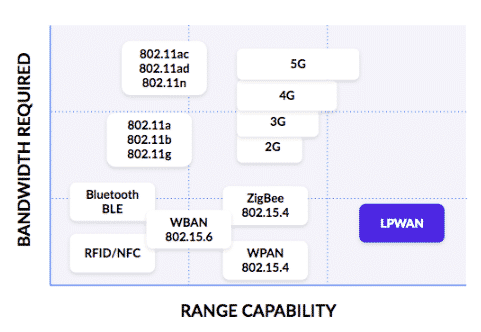
\includegraphics[width=0.6\textwidth]{img/LPWAN_comp.png}
			\caption{Comparativa entre LPWAN, en términos de alcance y ancho de banda, con respecto a otras comunicaciones inalámbricas [\ref{bib: iotforall lpwan options}].}
			\label{LPWANs vs otros}
		\end{center}
	\end{figure}

	\pagebreak
	
	\subsubsubsection{Comedero}
	\label{subsubsubsection: comedero busqueda}
	
	\noindent Tanto en este apartado, como en el siguiente sobre búsqueda de soluciones para el bebedero, se mostrarán opciones de sensores y actuadores para llevar a cabo sus funcionalidades asociadas.\\
	
	\noindent Para llevar a cabo la función de comedero, el sistema de alimentación creado debe ser capaz, en resumen, de mover el pienso de la reserva al comedero. Para ello, debemos tener en cuenta: 
	
	\begin{itemize}
		\item La capacidad de la reserva de pienso, y del comedero.
		\item Si la reserva quedará fija o móvil, y su soporte en todo caso.
		\item Cómo se gestionará el movimiento entre el pienso y el comedero; principalmente, las opciones más directas son movimiento basado en la gravedad, o movimiento gestionado por un motor. También será necesario estudiar el camino que realizará el pienso, para establecer conductos por donde pueda fluir hasta el comedero sin gran dificultad (lo que entendemos por \textit{conexionado entre reserva y comedero}).
		\item Soporte de los conductos que conectan la reserva y comedero.
		\item Conexionado eléctrico con el microcontrolador para recibir las señales de movimiento, en el caso de usar servo, o sensorización de niveles de pienso en reserva y/o en comedero.
	\end{itemize}
	
	\noindent Teniendo presente los puntos recién expuestos, se explicará brevemente en qué consisten aquellos sensores/actuadores que con mayor probabilidad podrán ser empleados. \\
	
	\noindent \textit{Servomotor} \\
	
	\noindent Un servomotor es... \\
	
	\noindent Algunos parámetros a tener en cuenta son... \\
	\noindent Stall current. Máxima corriente que se genera cuando el motor está aplicando su máximo torque. Free current. Corriente que se genera cuando el motor está girando libremente a su máxima velocidad, sin otra carga que la propia fricción y fuerzas contralectromotrices (\textit{back-EMF}). \\
	
	\pagebreak
	
	\subsubsubsection{Bebedero}
	
	\noindent De manera análoga a \ref{subsubsubsection: comedero busqueda}, para cubrir esta funcionalidad necesitaremos conseguir la manera de mover agua desde la reserva hasta el bebedero. Para ello: \\
	
	\noindent Opciones: ultrasónico en la tapa de la reserva + bomba + relé, sensores de nivel de agua (flotación) + relé + bomba. [Introducción en el apartado de Búsqueda de soluciones, pero todavía no está ordenado]\\
	
	\noindent \textit{Sensor ultrasónico}\\
	
	\noindent \textit{Bomba de agua} \\
	
	\noindent \textit{Sensores de nivel de agua} \\
	
	\noindent \textit{Relé} \\
	
	\noindent Un relé es un interruptor electromecánico que se conmuta (cambia de estado) mediante una señal eléctrica, y es digital, ya que sólo puede tomar el valor abierto y el cerrado (1 o 0, True o False). Sería algo parecido a un pulsador, pero sustituyendo el gesto mecánico de un dedo pulsando por una señal eléctrica. De esta forma, mediante una señal eléctrica de poca intensidad podemos controlar un circuito de mucha mayor potencia, aislando la parte de control. \\
	
	\pagebreak
	
	\begin{figure}
		\begin{center}
			\begin{tabular}{cc}
				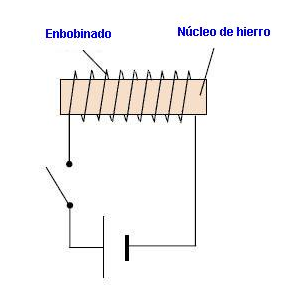
\includegraphics[width=60mm]{img/rele_1.png} &   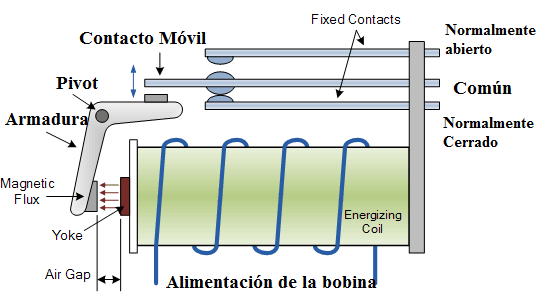
\includegraphics[width=80mm]{img/rele_2.png} \\
				(a)  & (b)  \\[6pt]
			\end{tabular}
			\caption{Imágenes que muestran las partes fundamentales de las que consta un relé [\ref{bib: prometec relés (más info)}].}
			\label{Rele: teoria}
		\end{center}
	\end{figure}

	\noindent El circuito de la Figura \ref{Rele: teoria}(a) muestra la base de un relé; consiste sencillamente en un núcleo de hierro (ferromagnético) y un cable conductor eléctrico, arrollado alrededor del núcleo, que se conecta a una batería de corriente continua. Si cerramos el interruptor, en el hierro se induce un campo  magnético sostenido, siguiendo las reglas de las leyes de Maxwell. Es decir se convierte en un electroimán. Si el núcleo no está sujeto a las espiras devanadas, se desplazará lateralmente, y si está sujeto el conjunto se comporta como un imán que podemos encender y apagar, lo que aprovechamos, para construir los relés.
	
	\noindent Fijándonos en la Figura \ref{Rele: teoria}(b), podemos observar que, cuando damos tensión a la bobina, el electroimán atrae la armadura haciéndola bascular alrededor del pívot, lo que desplaza el contacto móvil hacia arriba conectando el pin \textit{normalmente abierto} con el \textit{común} cerrando el circuito. A este contacto se le llama normalmente abierto (NA), porque el circuito entre el común y el pin NA, esta normalmente abierto (o sin conexión) hasta que se activa el relé. Por el mismo motivo hablamos del normalmente cerrado (NC), ya que el contacto está cerrado cuando el relé no está excitado. Cuando la bobina pierde la alimentación, el efecto imán desaparece y un resorte devuelve la armadura a la posición de reposo. A este tipo de relé, se le llama de armadura.
	
	\noindent Se podría llegar a pensar que los relés deberían tener 4 contactos, dos para la alimentación y dos para cerrar el circuito. Aunque existen, esto tendría el problema de que habría que fabricar un modelo NC y otro NA lo que supone un coste de fabricación mayor. Por eso, la mayor parte de los relés son de 5 pines, 2 se usan para conmutar el relé y los otros tres son el común y los pines NA y NC (al final un relé es un mecanismo, en el que una parte móvil metálica, cierra un contacto o lo abre). \\
	
	\noindent Seguramente la funcionalidad de un relé recuerde un poco a los transistores, pero tienen finalidades diferentes:
	
	\begin{itemize}
		\item Hay límites en la corriente que puede aceptar un transistor, sin embargo se pueden diseñar relés para aguantar cualquier carga.
		\item El relé aísla completamente el circuito de control del de potencia, algo muy importante para tensiones altas. Utilizaremos relés cuando tengamos cargas de mucha potencia.
		\item Un transistor conmuta (pasa de corte a saturación o viceversa) millones de veces más rápido que un relé.  Utilizaremos un transistor para cargas pequeñas y cuando la velocidad de conmutación sea importante.
		\item Sin embargo, hay que tener en cuenta que el relé cuenta con mayor desgaste, ya que cada vez que conmuta implica el movimiento de partes móviles mecánicas.
	\end{itemize}
	
	\noindent Tanto los transistores como los relés tiene la ventaja de disponer de un circuito de baja (control), y otra circuito de alta (carga), por lo que se aísla eficazmente el circuito de control, normalmente de baja tensión, como nuestro Arduino, del circuito de carga elevada que puede ser un motor de una cierta potencia, y por consecuente, capaz de inhabilitar nuestros circuitos de control. Por eso, cuando se manejan media y alta tensión en la industria, se suelen usar relés para conseguir aislamiento galvánico, por razones de seguridad, y se exige aislar la tierra del circuito de potencia y el negativo o GND del circuito de control, garantizando así el aislamiento galvánico de los dos circuitos. En el mundo Arduino se suelen usar relés de baja potencia, como mucho tensiones alternas alternas de 220V y máximo 5A para pequeños motores.
	
	\noindent Aunque hay muchos tipos de relés, por regla general nuestro Arduino no tiene potencia suficiente para activar un relé. Utilizaremos un transistor para amplificar la señal de la base y así poder conmutar el relé. El ejemplo que veremos a continuación incluye un circuito de transistor/relé completo que nos podrá valer para  cualquier proyecto que lo requiera.
	
	\begin{figure}[h]
		\begin{center}
			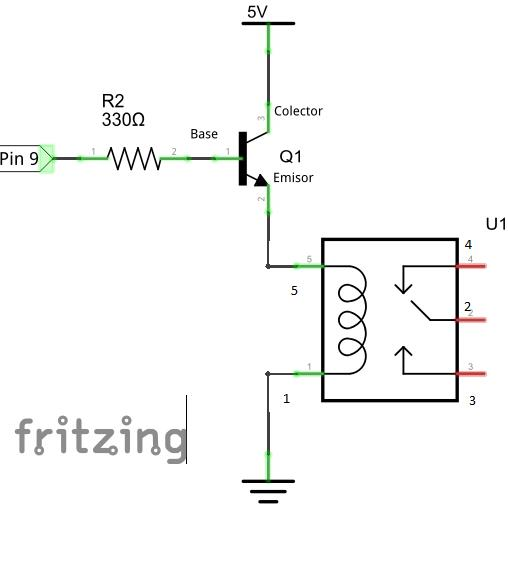
\includegraphics[width=0.4\textwidth]{img/rele_transistor.jpg}
			\caption{Ejemplo de circuito que emplea relé y un transistor entre relé y pin 9 de un arduino [\ref{bib: prometec relés y arduino}]}
			\label{Ejemplo rele con transistor}
		\end{center}
	\end{figure}
	
	\begin{itemize}
		\item Cuando hay un valor HIGH en el pin de control,  el transistor pasa a saturación  y la corriente entre emisor y colector excita la bobina del relé, haciendo que el contacto cambie de posición (y haciendo además un clic muy característico).
		
		\item Si hay un valor LOW en el pin de control el transistor entra en corte e impide el flujo de corriente por lo que la bobina cae y el contacto de salida vuelve a su posición de reposo.
		
		\item La salida del relé consta de 3 pines y no de dos como se podría esperar.  El motivo es que la conexión entre los pines de salida 2 y 3 es de tipo normalmente abierto (circuito abierto sin excitar) y entre los pines 2 y 4 es normalmente cerrado (circuito cerrado sin excitar la bobina).

	\end{itemize}
	
	\pagebreak
	
	\subsubsection{Prototipo exterior}
	
	\noindent Se trata de una funcionalidad que depende muy estrechamente de las funcionalidades presentadas anteriormente, por lo que para materializar una solución apta habrá que solventar las funcionalidades que le preceden. Se hablará más en detalle en el apartado \ref{subsubsection: prototipo exterior}, una vez se haya expuesto la elección de soluciones para las funcionalidades de alimentación autónoma y automatización y monitorización.
	% Definición funcionalidades: qué debo hacer y qué necesitaría
	% Investigación componentes (*) e integración (programación)
		%(*) Qué se ha usado, desglosado por funcionalidades: bebedero, comedero, alimentación, microcontrolador y radio.
		% Descripción, foto, foto en prototipo protoboard
	% Definición prototipo provisional: opciones que he descartado, QR de que funciona?
	% Diseño PCB
	% Desarrollo BBDD en servidor y app web para ver el estado del sistema de alimentación
	\pagebreak
	
	\subsection[Elección soluciones]{Elección de soluciones para cada funcionalidad}
	\label{Subsección 3.3: elección de soluciones para cada funcionalidad}
	
	\subsubsection{Alimentación autónoma del dispositivo}
	
	\noindent Para conseguir el objetivo de una alimentación autónoma para el dispositivo de alimentación final que queremos crear, se ha decidido usar la siguiente combinación de componentes, explicados de manera teórica y más ampliamente en el apartado \ref{subseccion 3.2.1: búsqueda soluciones alimentación}.
	
	\begin{figure}[h!]
		\begin{center}
			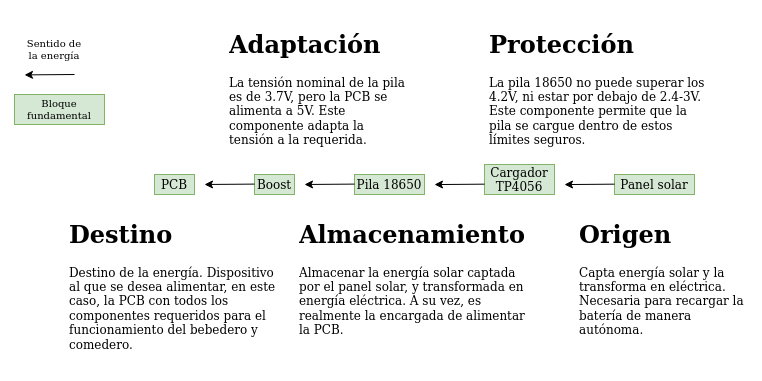
\includegraphics[width=0.75\textwidth]{img/conexiones tfg-alimentacion.png}
			\caption{Esquema general de la alimentación elegida para este proyecto.}
			\label{Alimentación: esquema general}
		\end{center}
	\end{figure}
	
	\begin{figure}[h!]
		\begin{center}
			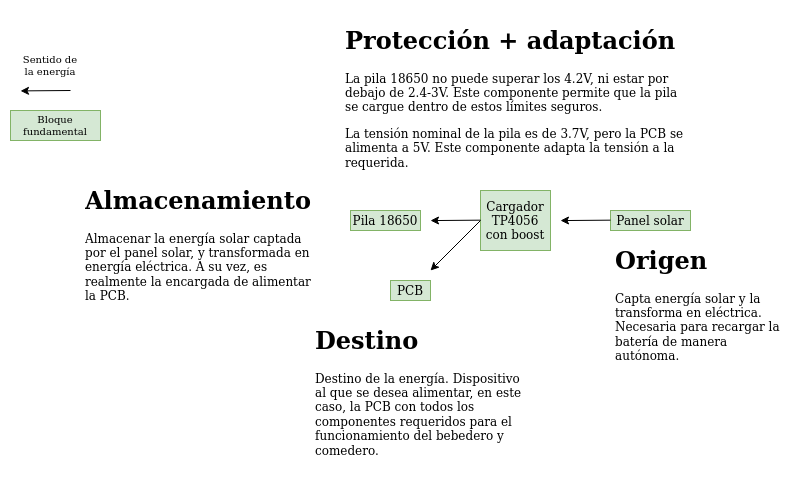
\includegraphics[width=0.75\textwidth]{img/conexiones tfg-alimentacion (boost en tp).png}
			\caption{Esquema general de la alimentación elegida para este proyecto (TP4056 con boost incluido).}
			\label{Alimentación: esquema general (tp con boost)}
		\end{center}
	\end{figure}
	
	\pagebreak
	
	\noindent Así pues,  se adquirieron los siguientes componentes: 
	
	\begin{itemize}
		\item \textbf{Batería recargable Li-ion 18650 sin protección.} Con tensión nominal de 3.7V, para un proyecto en el que las tareas de máximo consumo (rellenar comedero y envío de datos por LoRa) se van a ejecutar, como máximo, dos veces al día (en coste temporal, serán 5 minutos en total), en principio, pueden ser suficientes.
		\item \textbf{Kit protección 18650}, para pilas sin protección. Las pilas que vienen sin protección conllevan, como mínimo, una ausencia de protección contra cortocircuitos, es decir, si eléctricamente se conectan sus polos podemos dejar inservible la pila.
		\item \textbf{TP4056 con boost a 5V.} Al tener una tensión nominal de 3.7V, y requerir nuestro proyecto de una alimentación de 5V, necesitaremos algún elemento que eleve esta tensión, que, en nuestro caso, será un boost. No vendrá aislado, ya que lo usaremos en conjunto dentro de una PCB que corresponde a un módulo de carga de baterías li-ion llamado TP4056.
		\item \textbf{Panel solar 6V.} Se ha escogido un panel solar que, en teoría, nos da una tensión mínimamente funcional, de tamaño reducido para un primer prototipo y aproximación a la energía solar. Nos permitirá añadir la opción de recargar la batería de manera autónoma.
	\end{itemize}

	\noindent El elemento \textit{PCB} de la Figura \ref{Alimentación: esquema general (tp con boost)} será explicado más adelante, en la Sección \ref{Section: prototipo y pruebas}. A continuación, se muestran los pasos seguidos para montar el sistema de alimentación autónoma para nuestro dispositivo de alimentación para animales. \\
	
	\subsubsubsection{Preparación de la alimentación autónoma del dispositivo}
	
	\noindent Lo primero fue dejar asegurada la pila. Como se indica, la batería 18650 no tiene protección. Esto significa que cualquier manipulación incorrecta de la misma puede derivar en la rotura de la pila, o incluso en que ésta se inflame. Es por ello que se hizo uso de un kit para protección de baterías 18650, como el que se muestra en la Figura \ref{Proteccion kit Li-Ion}.\\
	
	\pagebreak
	
	\begin{figure}[h!]
		\begin{center}
			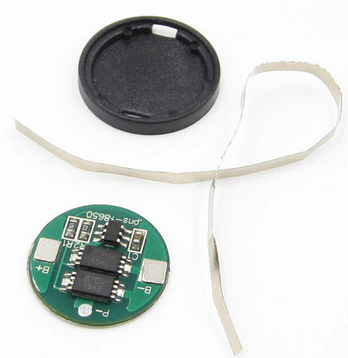
\includegraphics[width=0.4\textwidth]{img/proteccion_18650.png}
			\caption{Detalle del kit de protección para una batería 18650, a falta de tubo termoretráctil y contactos para los polos [\ref{bib: aliexpress dual mos}].}
			\label{Proteccion kit Li-Ion}
		\end{center}
	\end{figure}
	
	\noindent La protección que se ha añadido con este kit viene determinado por ciertos componentes electrónicos (como el que muestra la Figura \ref{Proteccion kit Li-Ion}), pero, además, por el recubrimiento metálico y plástico que se ha añadido a su alrededor. La construcción de la protección alrededor de la batería 18650, a través del kit adquirido, un termoretráctil y dos contactos metálicos para ambos polos, se resumen en la Figura \ref{Proteccion Li-Ion}. \\
	
	\begin{figure}[h!]
		\begin{center}
			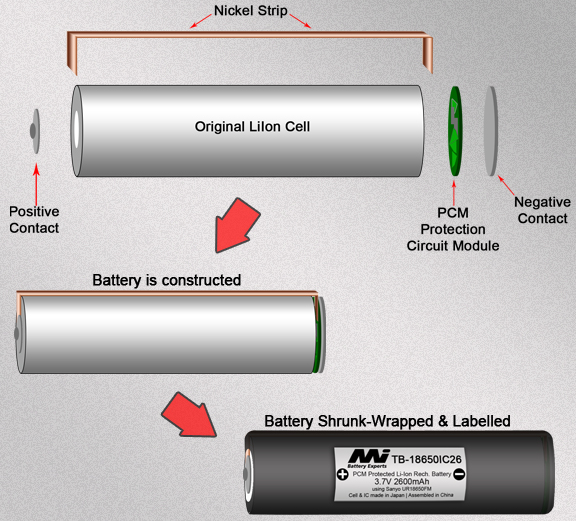
\includegraphics[width=0.5\textwidth]{img/construction_prot_circuit.png}
			\caption{Esquema de la protección que se añade a las pilas Li-ion [\ref{bib: protected li-ion cells}].}
			\label{Proteccion Li-Ion}
		\end{center}
	\end{figure}
	
	\pagebreak
	
	\noindent Sin entrar en mucho detalle, esta PCB (Figura \ref{PCB proteccion Li-Ion}) que incluye el kit (\textit{PCM}, según la Figura \ref{Proteccion Li-Ion})  actúa como protección extra para la batería en tanto a cortocircuitos, sobrecarga, sobredescarga y exceso de corriente. La batería incluye interiormente cierta protección, pero siempre es recomendable que si la batería no cuenta con este kit, se le añada (o se adquiera con él ya incluido y no añadirlo nosotros). Se ha señalado en la imagen, con un rectángulo rosa, el conjunto de dos MOSFET (8205A) que actúan como switches en las situaciones anteriormente mencionadas (por ejemplo, si hay exceso de corriente, corta el flujo, como un interruptor); señalado con el rectángulo verde, el circuito integrado DW01A, que permite realizar la lógica necesaria para detectar estos casos y actuar en consecuencia. 
	
	\begin{figure}[h!]
		\begin{center}
			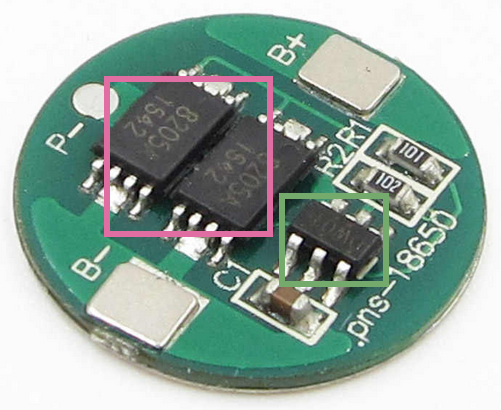
\includegraphics[width=0.3\textwidth]{img/batt_prot_circuit_zoom_edited.png}
			\caption{Detalle de la PCM de protección de la batería 18650 [\ref{bib: aliexpress dual mos}].}
			\label{PCB proteccion Li-Ion}
		\end{center}
	\end{figure}
	
	\noindent Finalmente, se muestra en la Figura \ref{18650 con y sin proteccion} fotos de la pila que se ha usado en este proyecto, antes de ponerle protección y después.
	
	\begin{figure}[h!]
		\begin{center}
			\begin{tabular}{cc}
				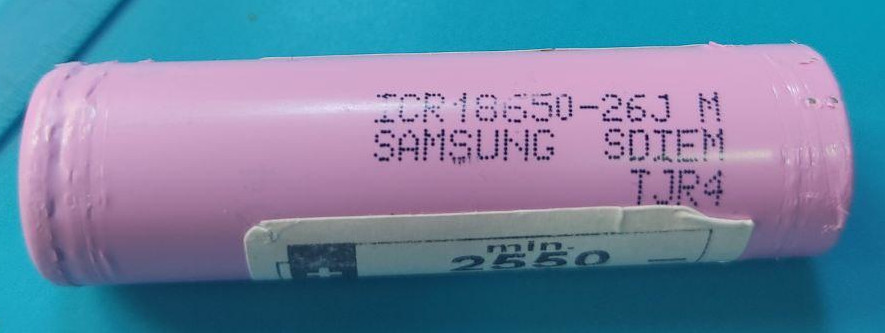
\includegraphics[width=40mm]{img/18650_sinProteccion.jpg} &   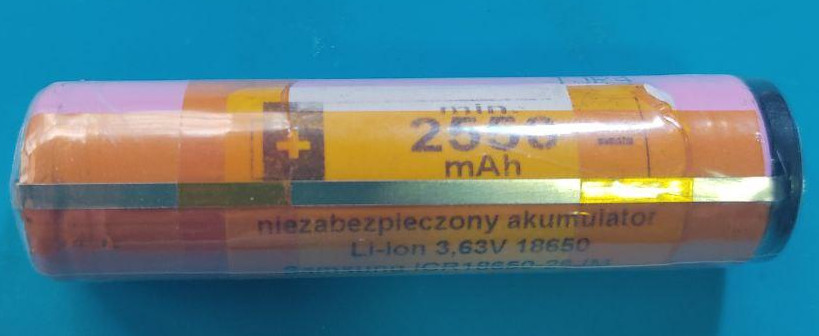
\includegraphics[width=40mm]{img/18650_conProteccion_1.jpg} \\
				(a) & (b) \\[6pt]
				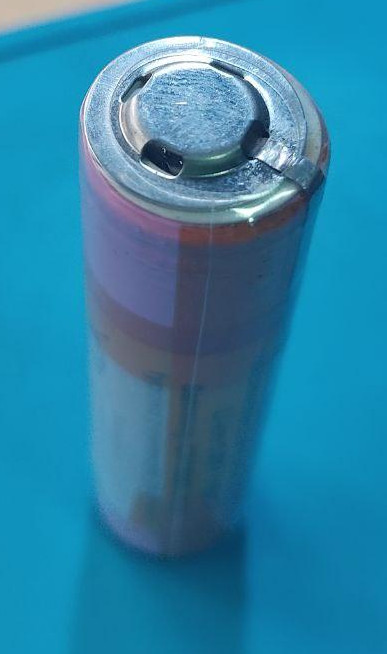
\includegraphics[width=25mm]{img/18650_conProteccion_2.jpg} &   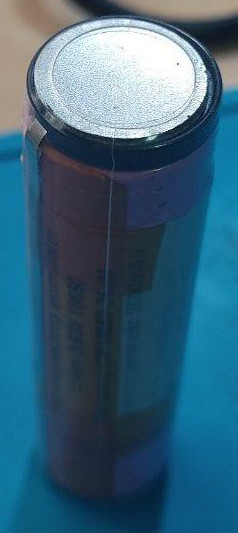
\includegraphics[width=20mm]{img/18650_conProteccion_3.jpg} \\
				(c)  & (d)  \\[6pt]
				%\multicolumn{2}{c}{\includegraphics[width=50mm]{img/} }\\
				%\multicolumn{2}{c}{(e) Pieza 5 PVC}
			\end{tabular}
			\caption{Fotos de la batería 18650 usada (sin protección, y con protección añadida).}
			\label{18650 con y sin proteccion}
		\end{center}
	\end{figure}
	
	\pagebreak
	
	\noindent Como se indicó en el apartado \ref{subseccion 3.2.1: búsqueda soluciones alimentación}, dentro de \textit{opciones para baterías recargables}, se necesita de un circuito que ayude a la pila, hecha de Li-ion, a una correcta carga y descarga, precisamente porque conlleva las mismas consecuencias de una mala manipulación, expuestas anteriormente. \\
		
	\noindent \textbf{TP4056} \\

	\noindent Es un circuito integrado que se emplea para gestionar la carga de la batería Li-ion.  Realmente, es una PCB donde encontramos el IC TP5046, junto con más componentes, pero de aquí en adelante hablaremos de TP4056 como la PCB global. Su funcionamiento, a grandes rasgos, consiste en transformar la fuente de energía eléctrica que tiene a su entrada para cargar la batería que tiene conectada a su salida; debido a que las baterías requieren que la energía sea cualitativa y cuantitativamente de una manera concreta, este paso es necesario. Además, también controla la temperatura. Las fuentes de energía eléctrica pueden ser diversas, desde un adaptador conectado a la red eléctrica, una fuente de alimentación, un panel solar, un generador, etc. No en todos los casos se necesitan los mismos componentes, depende de cada caso.\\
	
	\noindent Un ejemplo de TP4056 sencillo y fácil de encontrar sería el siguiente:  

	\begin{figure}[h]
		\begin{center}
			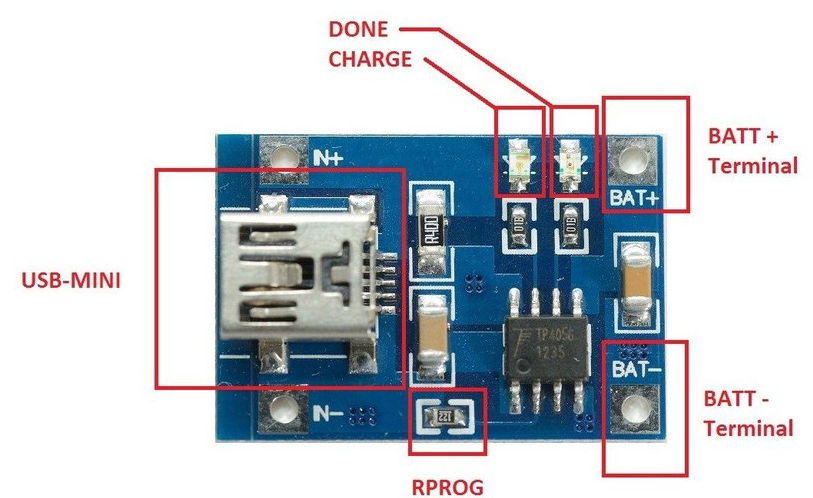
\includegraphics[width=0.6\textwidth]{img/tp4056_withoutBoost.png}
			\caption{Ejemplo de un TP4056 simple [\ref{bib: hwlibre TP4056}].}
			\label{TP4056 sin boost}
		\end{center}
	\end{figure}
	
	\noindent Del esquema anterior del módulo TP4056, podemos destacar: 
	
	\begin{itemize}
		\item \textbf{Puerto mini-USB}: para alimentar la batería a través de este tipo de cables. Lo usaremos si deseamos cargar la batería de manera externa al proyecto.
		\item \textbf{Bornas IN-, IN+}: están a los lados del puerto. Sirven también para alimentar la batería. A estas bornas podemos conectar una placa solar, u otra fuente que se necesite. En nuestro caso, será el panel solar de 6V.
		\item \textbf{LEDs de carga y completado}: avisarán cuando la batería esté cargándose o cuando haya terminado dicho proceso.
		\item \textbf{BAT+ y BAT-}: son bornas de salida que irán conectados a la batería que se necesita cargar.
	\end{itemize}

	\noindent Sin embargo, se requieren más elementos para alimentar al dispositivo, como por ejemplo un conversor de tensión tras la batería (entre batería y dispositivo). En nuestro caso, lo requerimos, ya que la batería usada otorga 3.7V nominales (no existen baterías de 5V) y nosotros necesitamos 5V para alimentar el sistema de alimentación. Necesitamos un elemento que nos aumente la tensión a su salida, para alimentar de manera correcta el sistema creado; usaremos, por tanto, un \textit{boost converter}. Es un dispositivo que puede encontrarse aislado, aunque también podemos encontrarlo en una misma PCB con el TP4056, y será esta última opción la que usemos. \\
	
	\begin{figure}[h]
		\begin{center}
			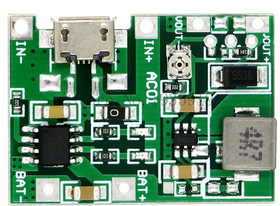
\includegraphics[width=0.3\textwidth]{img/tp4056_withBoost.png}
			\caption{Ejemplo de un TP4056 con boost [\ref{bib: aliradar tp4056 con boost}].}
			\label{TP4056 con boost}
		\end{center}
	\end{figure}
	
	\noindent Vemos que cuenta con los elementos principales anteriormente mencionados (bornas IN+ e IN-, bornas VOUT + y VOUT-, bornas BAT- y BAT
	+, micro USB y LEDs). Cuenta con 2 IC's principalmente: el TC4056A y el B6289A. El primer IC viene a ser uno con funcionamiento similar al TP4056, y el segundo es el encargado de la función de boost. Cabe señalar que contamos con un potenciómetro con el que podemos variar la corriente con la que se cargará la batería (página 6 del datasheet del TC4056). 
	
	%Problema: no tiene protección contra sobredescargas. \\

	
	\noindent Para compactar este conglomerado (pila  con TP4056), se han unido soldando las conexiones entre ellos en una placa experimental, como la que se muestra en la Figura \ref{Componentes conglomerado}(a). En concreto, se ha soldado el TP4056 de la Figura \ref{TP4056 con boost} con conectores de tipo screw terminal (Figura \ref{Componentes conglomerado}(b)); de esta manera, conectaremos el panel solar a través de sus cables a un screw terminal, el cual unirá mediante soldadura a las bornas IN+ e IN-, y lo mismo sucederá con la pila.
	
	\pagebreak
	
	\begin{figure}[h!]
		\begin{center}
			\begin{tabular}{cc}
				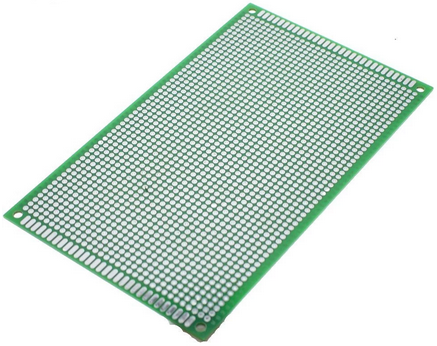
\includegraphics[width=50mm]{img/placa_exp.png} \label{Ejemplo placa experimental} &   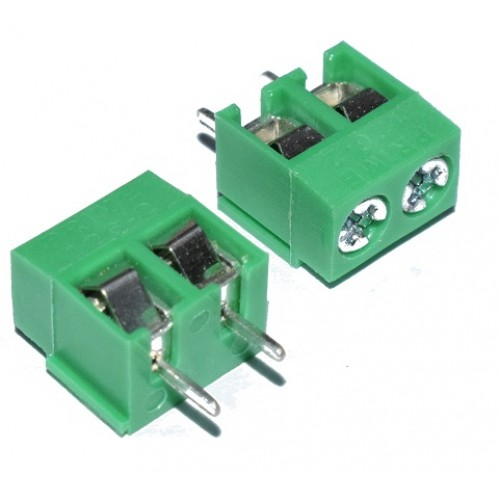
\includegraphics[width=40mm]{img/screw.jpg}  \label{Ejemplo screw} \\
				(a) Placa experimental [\ref{bib: aliexpress placa exp}] & (b) Screw terminal [\ref{bib: rarecomponents screw}] \\[6pt]
				%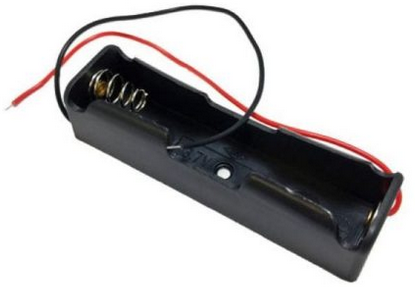
\includegraphics[width=50mm]{img/18650_holder.png}  \label{Ejemplo holder 18650} &   %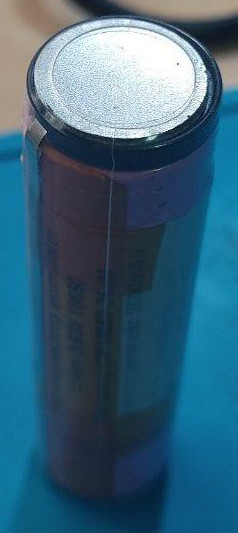
\includegraphics[width=20mm]{img/18650_conProteccion_3.jpg} \\
				%(c) Holder para una batería 18650\\ [6pt]
				\multicolumn{2}{c}{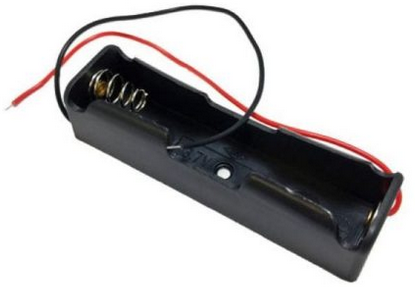
\includegraphics[width=50mm]{img/18650_holder.png} \label{Ejemplo holder 18650} }\\
				\multicolumn{2}{c}{(c) Holder para una batería 18650 [\ref{bib: solarbotics holder para 18650}]}
			\end{tabular}
			\caption{Elementos que formarán nuestro conglomerado provisional de alimentación del dispositivo.}
			\label{Componentes conglomerado}
		\end{center}
	\end{figure}

	\noindent [Foto real de cómo ha quedado, y otra foto conectando todo, hasta panel solar]. \\
%	\begin{figure}[h]
%		\begin{center}
%			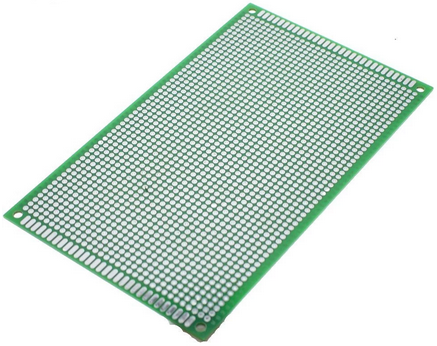
\includegraphics[width=0.4\textwidth]{img/placa_exp.png}
%			\caption{Ejemplo de una placa experimental [\ref{bib: aliexpress placa exp}].}
%			\label{Ejemplo placa experimental}
%		\end{center}
%	\end{figure}

	\subsubsection{Automatización y monitorización}
	
	\noindent Para la automatización y monitorización del sistema de alimentación, se ha elegido, en tanto a los bloques de microcontrolador y  comunicación radio, las tecnologías Arduino y LoRa, respectivamente. Si bien estas elecciones se habrían realizado a priori por ser opciones \textit{Open Source} muy extendidas y conocidas por la comunidad, no ha supuesto que no se investiguen otras, las cuales se han mencionado en el apartado \ref{subsección 3.2.2: automatización y monitorización}.
	
	\subsubsubsection{Entorno Arduino}
	
	% Intro: qué es Arduino
	
	\noindent [Anotaciones: usamos una versión diferente a la de Arduino nano vendida por la organización Arduino. Seguramente lo mueva de aquí.] \\
	
	\noindent Usaremos un arduino nano que usa un ATmega328P y un chip CH340. En la sección X se han explicado las especificaciones técnicas, pinout y componentes que forman parte del arduino nano fabricado por la organización Arduino, pero el que va a ser usado lo está por otro fabricante. A efectos prácticos, las diferencias son pocas, pero hay que considerarlas de igual manera:
	
	\begin{itemize}
		\item El microcontrolador no es ATmega328 (usado en el nano de la organización Arduino), sino que es ATmega328P. La diferencia reside en que es una versión posterior diseñada para consumir menos potencia que el 328, esencialmente tienen la misma arquitectura y características en tanto a memoria flash, EEPROM y SRAM (la P viene de \textit{picoPower}).
		\item Este arduino usa un regulador diferente, el CH340G, frente al FT232 que usa el arduino original. Además, el fusible/diodo Schottky que usan para proteger la comunicación serial frente a sobrecorrientes es diferente, siendo el MBR0520 para el caso de los arduinos originales, frente al B5819W que usa el arduino que vamos a usar.
	\end{itemize}
	
	\noindent Arduino es una plataforma de electrónica \textit{open-source} basada en hardware y software fáciles de usar. Nació en el \textit{Ivrea Interaction Design Institute} (Italia) como una herramienta fácil para la creación rápida de prototipos, dirigida a estudiantes sin experiencia en electrónica y programación. Tan pronto como llegó a una comunidad más amplia, la placa Arduino comenzó a cambiar para adaptarse a las nuevas necesidades y desafíos, tanto de usuarios principiantes como expertos. \\
	
	\noindent Las placas Arduino son capaces, por una parte, de ejecutar una serie de instrucciones (determinadas por el usuario) a través de su microcontrolador, de manera que a partir de la lectura de sus entradas analógicas/digitales se puedan generar salidas (analógicas/digitales); por otra parte, son programables a través del software Arduino, lo que se conoce como Arduino IDE. \\
	
	\noindent \textbf{Características} \\
	
	\noindent La principal característica de Arduino es la simplicidad para trabajar con microcontroladores. A raíz de esto, ofrece una serie de ventajas para sus usuarios, como son:
	\begin{itemize}
		\item \textbf{Es de bajo coste}. Las placas de Arduino son relativamente de bajo coste comparadas con las plataformas de otros microcontroladores. La versión más económica de un módulo Arduino puede ser ensamblada a mano, e incluso los módulos Arduino pre-ensamblados cuestan menos de 50 \$.
		\item \textbf{Multiplataforma}. El software de Arduino, Arduino IDE, es capaz de ejecutarse en Macintosh OSX, Windows y Linux. La mayoría de sistemas de microcontroladores están limitados a Windows.
		\item  	\textbf{Entorno de programación simple y claro}. El software de Arduino (IDE) es fácil de usar para principiantes, sin dejar de ser lo suficientemente flexible para usuarios más avanzados.
		\item \textbf{Software Open Source y extensible}. El software Arduino está publicado como un conjunto de herramientas open source, disponible para ser ampliada por otros programadores a través de librerías basadas en el lenguaje C++; las personas que quieran comprender los detalles técnicos pueden dar el salto de Arduino al lenguaje de programación AVR C en el que se basa. Del mismo modo, se puede agregar código AVR-C directamente en los  programas Arduino si así se desea.
		\item \textbf{Hardware Open Source y extensible}. Los planos de las placas Arduino están publicados bajo licencia \textit{Creative Commons}, así pues, diseñadores de circuitos experimentados pueden hacer su propia versión del módulo, extendiéndola y mejorándola. Incluso usuarios sin experiencia pueden crear una versión en protoboard del módulo para entender cómo funciona y ahorrar dinero.
	
	\end{itemize}

	\noindent \textbf{Hardware: placas Arduino} \\
	
	\noindent Existen diferentes placas Arduino, cuya elección dependerá del objetivo que persiga nuestro proyecto y de los requerimientos y limitaciones sobre dicho proyecto. \\
	
	\noindent Algunas de las placas básicas de Arduino más usadas son Arduino nano, Arduino uno o Arduino mega. Nos centraremos en el Arduino nano, ya que es el que vamos a usar; aún así, ya se comentaron las especificaciones y características del Arduino uno en el apartado \ref{subsección 3.2.2: automatización y monitorización}, sección \textit{Microcontroladores}, como ejemplo de placa Arduino de cara a comparar con otras opciones de microcontrolador, por lo que no se volverá a explicar en esta sección.  \\
	
	\noindent \textit{Especificaciones del Arduino nano} \\
	
	\begin{itemize}
		\item Microcontrolador: ATmega328
		\item Arquitectura: AVR
		\item Tensión de funcionamiento: 5V
		\item Memoria flash: 32kB de los cuales 2kB son para el gestor de arranque (\textit{bootloader}).
		\item SRAM: 2kB
		\item Velocidad del reloj: 16 MHz
		\item Pines de entrada analógicos: 8
		\item EEPROM: 1 kB
		\item Corriente CC por pin de entrada/salida: 40mA (pines I/O)
		\item Tensión de entrada: 7-12V
		\item Pines digitales de entrada/salida: 22 (de los cuales 6 son PWM)
		\item Salida PWM (\textit{Pulse Width Modulation}): 6
		\item Consumo de energía: 19 mA
		\item Tamaño de la PCB: 18 x 45 mm
		\item Peso: 7g
	\end{itemize}
	
	\noindent \textit{Pinout del Arduino nano} \\
	
	\noindent La funcionalidad de cada uno de los pines analógicos y digitales se pueden ver en la Figura \ref{Pinout Arduino nano}. \\
	
	\begin{figure}[h]
		\begin{center}
			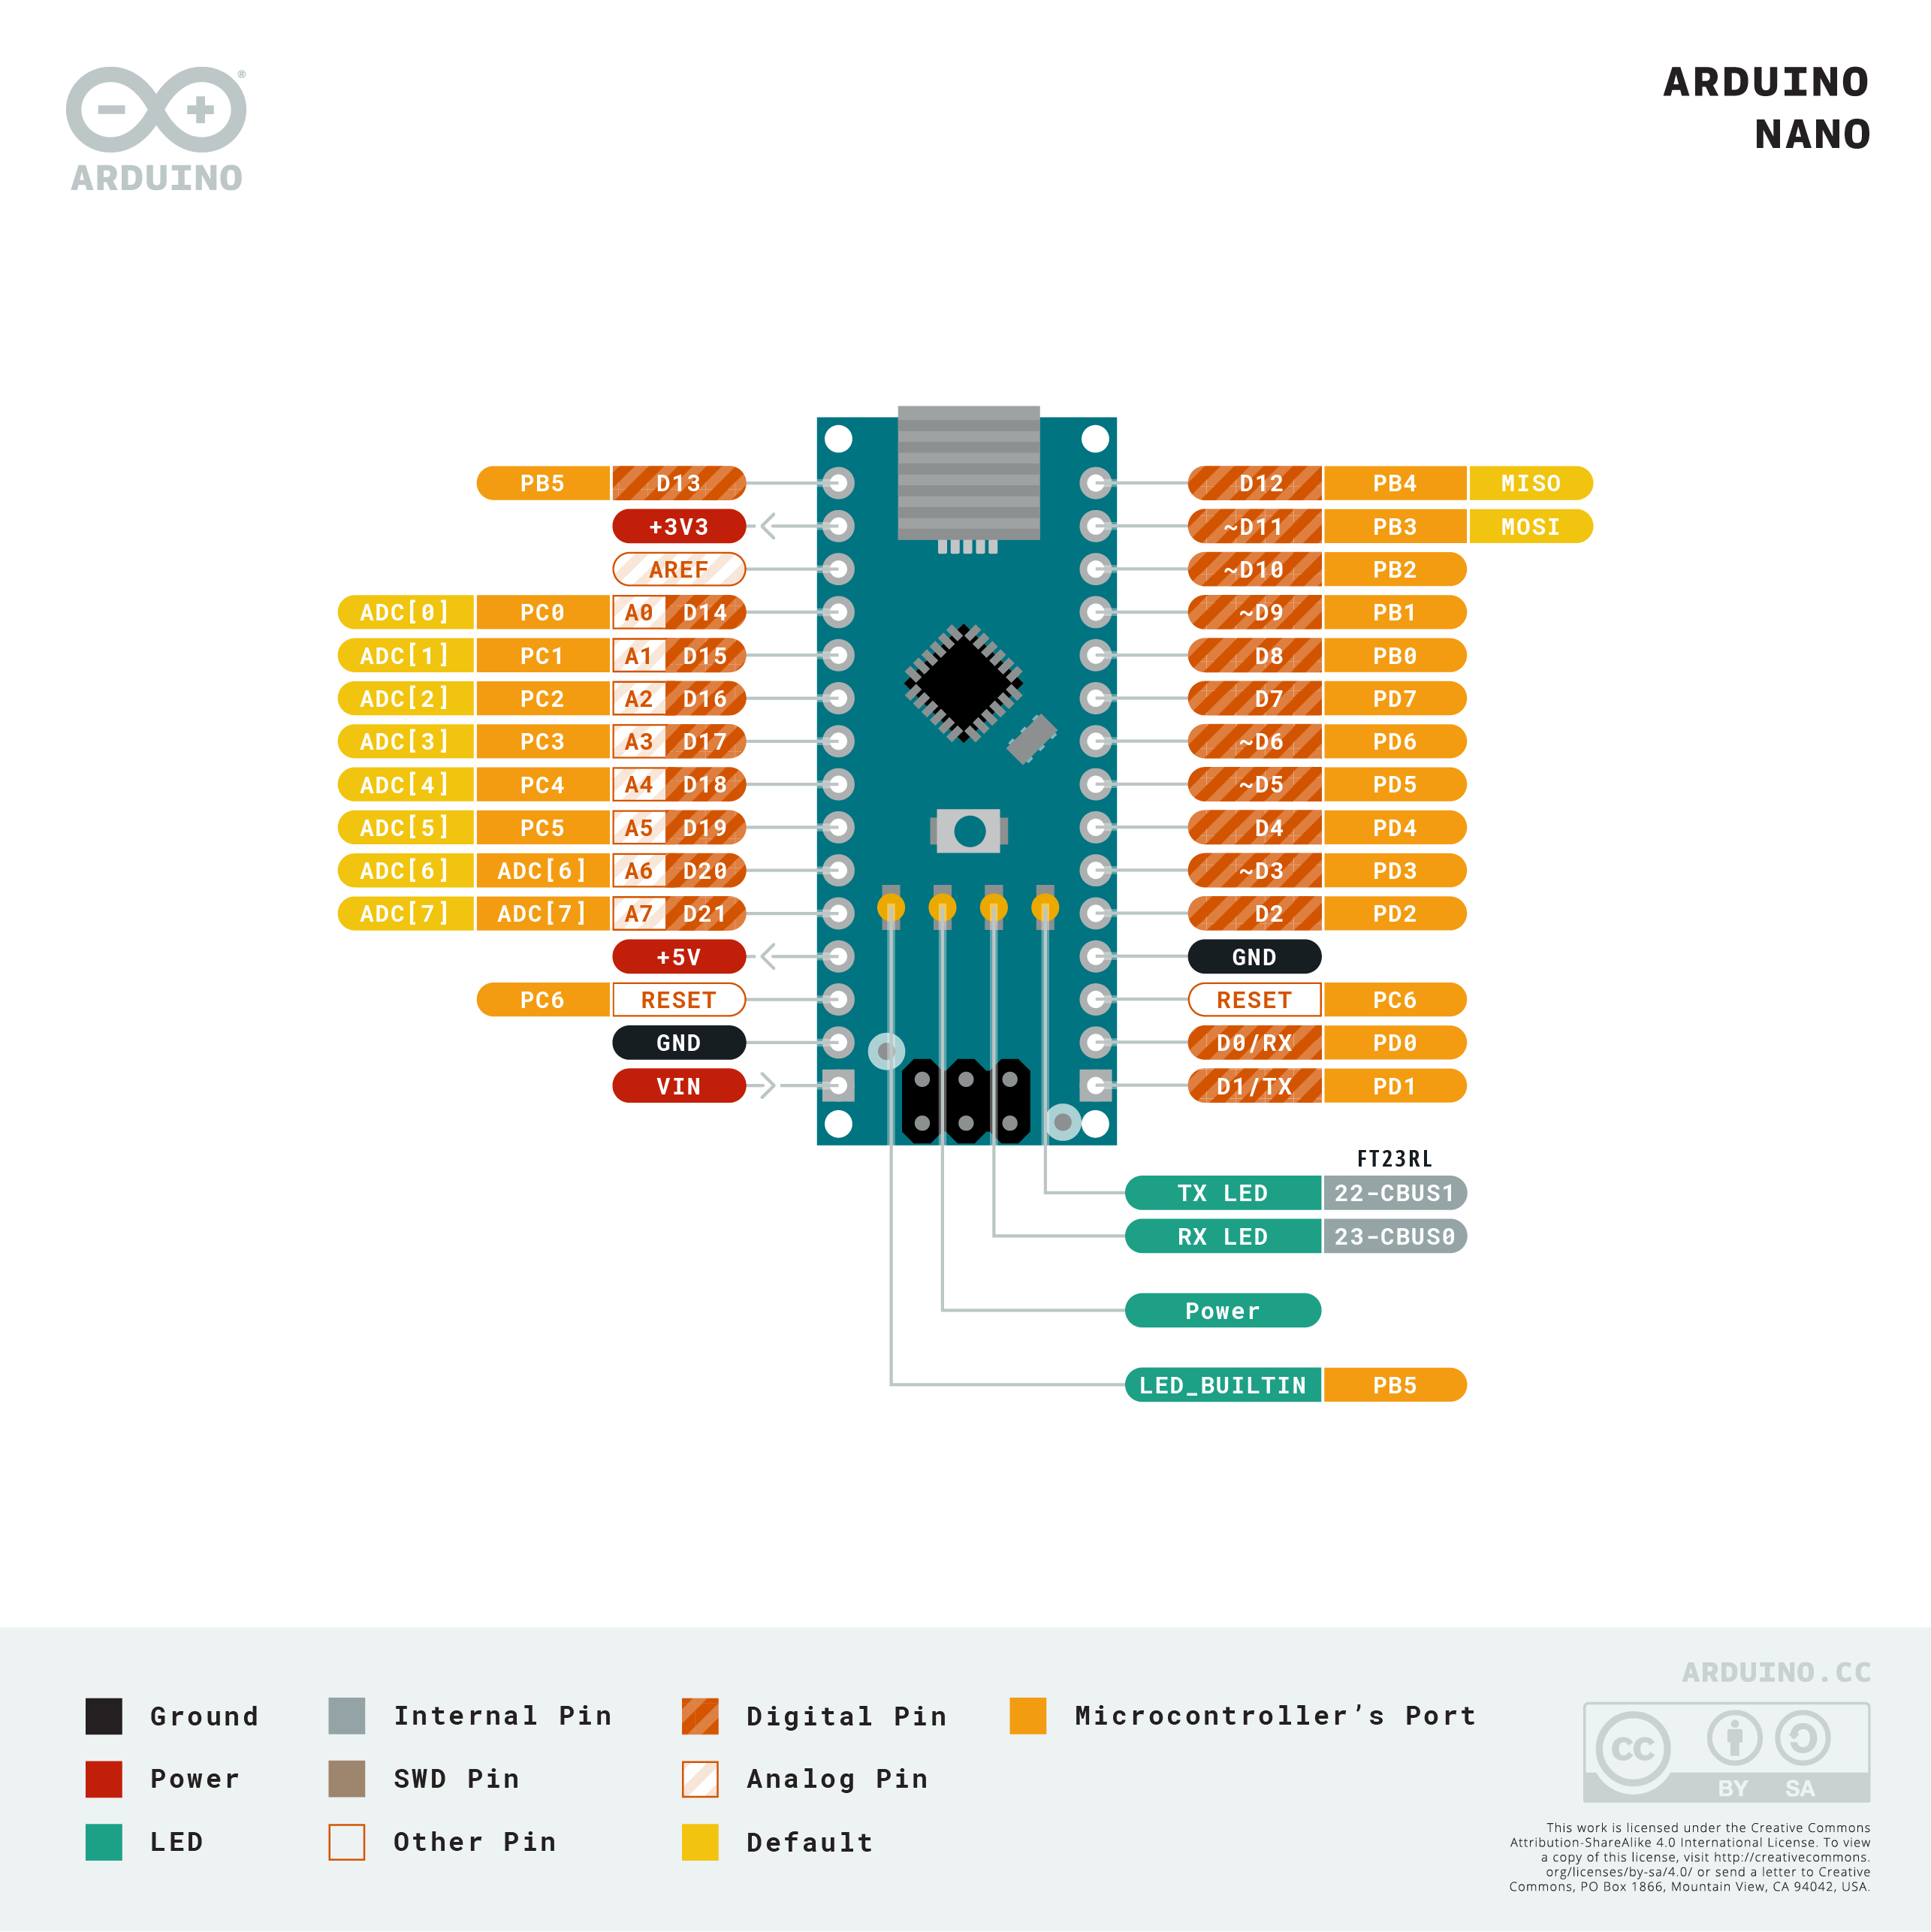
\includegraphics[width=0.7\textwidth]{img/Pinout-NANO_official.png}
			\caption{Pinout de un Arduino nano.}
			\label{Pinout Arduino nano}
		\end{center}
	\end{figure}

	\pagebreak
	
	\noindent Tendremos la misma cantidad de pines digitales configurables como entrada o salida (D2 a D13), donde 6 de ellos tendrán capacidad PWM, igual que arduino uno. Respecto a los pines analógicos tenemos los pines A0 a A5 igual que el modelo uno, pero aparecen dos pines adicionales, A6 y A7, consiguiendo así un total de 8 entradas analógicas. \\
	
	\noindent [Foto pines digitales y analógicos, señalando los que son PWM.] \\
	
	\noindent Los dos primeros pines de la esquina inferior derecha corresponden a D1 para TX y D0 para RX de la comunicación serie por UART(\textit{Universal Asynchronous Receiver-Transmitter}); en Arduino uno estos mismos pines también aparecían pero en orden invertido. Son un reflejo de las líneas de comunicación provistas por el conversor USB-TTL, aunque por lo general usamos la librería Software serial para definir otros dos pines cualquiera para dicha función. Ya que estamos hablando de comunicación serie, tenemos los pines asociados a la interfaz SPI (\textit{Serial Peripheral Interface}), iguales que en el modelo uno; el pin digital 10 ejecutando la función de slave select, el 11 como MOSI (\textit{Master Output Slave Input}), el 12 como MISO (\textit{Master Input Slave Output}) y el 13 como serial clock. Al igual que en el modelo uno, la interfaz de dos cables, I2C (\textit{Inter-Integrated Circuit}), estará presente en A4 para SDA (\textit{System Data}) y en A5 para SCL (\textit{System Clock}). \\
	
	\noindent [Foto pines digitales y analógicos, señalando los especiales para comunicaciones SPI, I2C y UART.] \\
		
	\noindent El resto de pines: Salida de 3,3V. Referencia de las entradas analógicas AREF. Salida regulada de 5V, usada normalmente para alimentar sensores y dispositivos, y dos pines de GND o masa en ambos lados de la placa. Un pin de RESET para realizar dicha función de forma remota si no tenemos acceso al pulsador físico de la placa. Finalmente, Vin se usará para alimentar la placa con una fuente no regulada de entre 7 y 12V; en arduino uno teníamos un conector para alimentación externa de tipo Jack, en arduino uno, como la placa tiene un tamaño reducido, no resultaría práctico colocar un conector tan voluminoso, por eso tenemos un pin destinado para alimentación externa. \\
	
	\noindent [Foto pines digitales y analógicos, señalando los especiales para comunicaciones SPI, I2C y UART, y pines de alimentación.] \\
	
	\noindent Pin de salida de 5V refleja los mismos 5V del puerto  del ordenador; si ahora deseamos trabajar de manera autónoma, sin conexión al ordenador, podremos alimentar la placa con una fuente externa con valores de tensión de entre 7 y 12 V. Dicha tensión se aplica de forma directa al regulador lineal de tensión, el cual convertirá la tensión de entrada no regulada a 5V regulados con un suministro máximo de corriente de hasta 500mA. Para la salida de 3.3V, es diferente en nano respecto de uno; en nano, los 3.3V son generados por el propio conversor USB-TTL (el circuito integrado lleva incorporado el regulador); el modelo uno dispone de un regulador por separado y destinado exclusivamente para el riel de 3.3V. En uno, dicho regulador puede suministrar hasta 150 mA de corriente máxima, mientras que en nano, como no tenemos un regulador especializado, y forma parte de la funcionalidad del conversor, el suministro de corriente será menor, de 50 mA como máximo. \\
	
	\noindent [Foto parte rear del nano señalando partes implicadas en la alimentación del nano.] \\
	
	\noindent \textit{Componentes que forman el Arduino nano} \\
	
	\noindent \textbf{Vista superior:} conector mini USB, más pequeño que el que usa arduino uno. El arduino nano tiene el mismo microcontrolador que el arduino uno (ATmega328P con encapsulado de montaje superficial), por lo que los programas/instrucciones que se desarrollen para uno son válidos/equivalentes para el otro. \\
	
	\noindent [Foto vista superior e inferior del Arduino nano.] \\
	
	\noindent \textbf{Vista inferior:} tenemos una tirada de pines macho para conectar a protoboard o a cables directamente. Difiere del arduino uno en este sentido, ya que el arduino uno tenía pines hembra en la parte superior. La idea principal para estos pines macho es conectarla a protoboard en un circuito impreso con un zócalo o soldado de forma directa.
	Cerca del conector USB tenemos un CI, un conversor USB-TTL, que nos permite conectar la placa al ordenador, obtener de él alimentación y comunicación para cargar programas y monitoreo serie. Finalmente, un regulador de tensión de 5V, permite obtener dicha tensión en un pin de salida para alimentar dispositivos externos cuando es alimentada la placa de forma externa mediante un pin especial llamado Vin.  \\

	\noindent \textit{Justificación de elección para el proyecto} \\
	
	\noindent Se ha elegido esta opción por una serie de razones, que a continuación se expondrán: \\
	
	\begin{itemize}
		\item Bajo consumo
		\item Precio reducido
		\item Facilidad para la incorporación a una PCB
		\item Tamaño reducido
		\item Amplia cobertura por la comunidad
		\item Open Source
	\end{itemize}
	

	\noindent Existen placas Arduino que incorporan conectividad IoT (no sólo LoRa, también WiFi, BLE, Bluetooth o Sigfox), como Arduino MKR FOX 1200, Arduino MKR WAN 1300, Arduino MKR WAN 1310, Arduino MKR NB 1500, Arduino Nano 33 BLE Sense, Arduino Uno WiFi REV2, Arduino MKR1000 WiFi, Arduino Nano 33 BLE, Arduino Nano 33 IoT, Arduino Nano 33 BLE, o Arduino MKR WiFi 1010.  Al ser soluciones ya integradas y muy concretas, orientadas más a redes LPWAN con conectividad a internet, no se han considerado como solución para este proyecto, pero se mencionan ya que se han estudiado y pueden resultar útiles para futuras investigaciones o proyectos similares.\\
	
	% Electrónica: arduino nano
	
	\noindent \textbf{Software: Arduino IDE} \\
	
	% Programación: arduinoIDE, void loop y setup, define, etc
	
	\noindent Como hemos mencionado anteriormente, las placas Arduino se pueden programar a través del software Arduino IDE. Además, A continuación, se explicarán los fundamentos básicos que se requieren para empezar a usar este software. \\
	
	\begin{itemize}
		\item Bloque de definición de variables globales.
		\item Bloque de definición de las tareas a realizar por el microcontrolador.
	\end{itemize}
	
	\subsubsubsection{LoRa}
	
	\noindent \textbf{Qué es}\\
	
	\noindent El término LoRa proviene de la unión de las palabras \textit{Long} y \textit{Range}, es decir, largo alcance, evidenciando, así, a través de su nombre una de sus principales características. Se trata de la capa física del protocolo \textit{LoRaWAN}; es a través de esta capa que se permite el establecimiento del enlace de comunicación de largo alcance, mientras que LoRaWAN define el protocolo de comunicación y la arquitectura del sistema para la red. \\
	
	\noindent También se trata de una tecnología inalámbrica propiamente dicha que ofrece una transmisión de largo alcance, bajo consumo y segura para aplicaciones IoT y M2M. Se basa en la modulación de espectro ensanchado, la cual presenta características de bajo consumo como la modulación FSK pero puede ser usada para comunicaciones de largo alcance. Puede ser usada para conectar sensores, gateways, máquinas, dispositivos, animales, personas, etc. de manera inalámbrica a la nube.\\
	
	\noindent \textbf{Planes de frecuencia} \\
	
	\noindent La tecnología LoRa opera en diferentes frecuencias dependiendo de la región en la que nos encontremos, por ejemplo: \\
	
	\begin{itemize}
		\item En Norteamérica, opera en la banda de 915 MHz.
		\item En Europa, en la banda de 868 MHz.
		\item En Asia, en la banda de 865 a 867 MHz y en la banda 920 a 923 MHz, aunque es común también la banda 433 MHz.
	\end{itemize}
	
	\noindent Dado que los planes de frecuencia para LoRa varían según la región, inclusive país, es recomendable asegurarse de las regulaciones vigentes en cada país para el uso del espacio radioeléctrico. A modo resumen y como orientación inicial a este asunto, se puede consultar esta \href{https://www.thethingsnetwork.org/docs/lorawan/frequencies-by-country/index.html}{lista de planes de frecuencia para cada país}, elaborada por \textit{The Things Network}. \\
	
	\noindent \textbf{Origen} \\
	
	\noindent La tecnología LoRa fue creada por una compañía francesa llamada \textit{Cycleo}, la cual posteriormente fue adquirida por Semtech en 2012. Semtech fue el miembro fundador de \textit{LoRa Alliance}, que actualmente es el organismo rector de LoRa Technology. LoRa Alliance es una de las alianzas tecnológicas de más rápido crecimiento. Esta asociación sin ánimo de lucro está formada por más de 500 empresas miembro, comprometidas a permitir la implementación a gran escala de redes IoT de amplia cobertura y baja potencia (LPWAN) a través del desarrollo y la promoción del estándar abierto LoRaWAN.\\
	
	\noindent \textbf{Especificaciones en términos generales de la tecnología LoRa}
	
	\begin{itemize}
		\item Órgano rector: LoRa Alliance
		\item Estándar: 801.15.4g
		\item Frecuencia: banda ISM, 868/916 MHz
		\item Alcance: hasta 5 km (urbano) y hasta 15 km (rural)
		\item Datarate: 27 kbps
		\item Modulación: espectro ensanchado basado en la tecnología de modulación FM
		\item Seguridad: CRC de 32 bits
	\end{itemize}
	 
	 %LoRaWAN is a Low Power, Wide Area (LPWA) networking protocol developed by the LoRa Alliance, that wirelessly connects battery operated ‘things’ to the internet in regional, national or global networks, targeting key Internet of Things (IoT) requirements such as bi-directional communication, end-to-end security, mobility and localization services.
	 
	% LoRaWAN uses unlicensed spectrum in the ISM bands to define the communication protocol and system architecture for the network while the LoRa physical layer creates the long-range communication links between remote sensors and gateways connected to the network. This protocol helps in the quick setup of public or private IoT networks anywhere using hardware and software.
	
	\noindent  \textbf{Regulación LoRa en Europa: ERC 70-03} \\
	
	\noindent \href{https://docdb.cept.org/download/25c41779-cd6e/Rec7003e.pdf}{ERC 70-03} \\

	\noindent \textbf{Transceptores LoRa elegidos: E32-868T30D} \\
	
	\noindent Los módulos LoRa que vamos a usar son los E32-868T30D. En la Figura \ref{fig: capturas E32.} se adjunta una imagen del dispositivo en cuestión. \\
	
	\begin{figure}[h]
		\begin{center}
			\begin{tabular}{cc}
				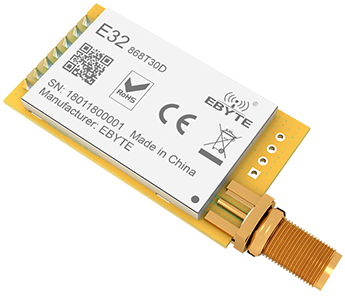
\includegraphics[width=60mm]{img/e32_front.png} &   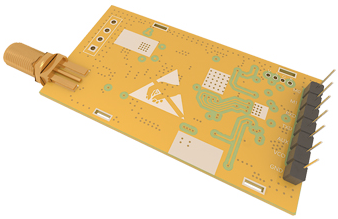
\includegraphics[width=60mm]{img/e32_rear.png} \\
				(a) Parte frontal & (b) Parte trasera\\[6pt]
			%	\multicolumn{2}{c}{\includegraphics[width=60mm]{img/Fotos comedero/helice_v3VSv2VSv1_rotated.png} }\\
			%	\multicolumn{2}{c}{(c) Versión 3 de las hélices (comparado con v1 y v2)}
			\end{tabular}
			\caption{Capturas del transceptor LoRa E32-868T30D [\ref{bib: imagen E32}].}
			\label{fig: capturas E32.}
		\end{center}
	\end{figure}	
	
	\noindent La ficha técnica de este dispositivo se puede consultar en el Anexo I. Destacaremos algunos parámetros en los que se ha basado su elección: \\
	
	\begin{itemize}
		\item 
	\end{itemize}
	
	\noindent Se usarán antenas de 5 dBi con diagrama de radiación tipo dipolo.\\
	
	\begin{figure}[h]
		\begin{center}
			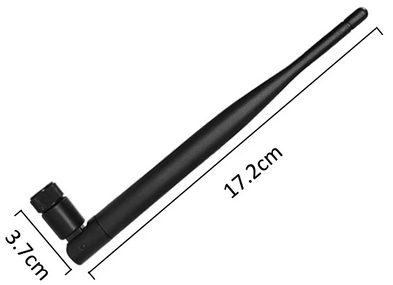
\includegraphics[width=0.3\textwidth]{img/antena_5dbi.png}
			\caption{Captura de las antenas usadas [\ref{bib: AliExpress}].}
			\label{Captura antenas 5dbi}
		\end{center}
	\end{figure}
	
	\noindent \textit{Simulación en Radio Mobile}\\
	
	\noindent Una vez elegidos los componentes (transceptores y antenas) y antes de realizar las pruebas de campo, es procedente simular el enlace radio con los parámetros de los componentes escogidos. Para ello, se empleó el programa de simulación \textit{Radio Mobile}. No simularemos únicamente los transceptores E32-868T30D, sino que, además, se simulará para el transceptor E22-900T22D, un transceptor que se comentó en el apartado de \textit{Búsqueda de soluciones}, y que además de tener una tecnología muy similar al E32, nos puede proporcionar el RSSI, un parámetro que nos ayuda a valorar la intensidad de la señal en recepción sin necesidad de otras herramientas (las cuales habría que comprar o tomar prestadas, calibrar, etcétera). El estudio en profundidad de este transceptor no entra dentro del alcance programado para este proyecto, sin embargo, se realizan las simulaciones correspondientes para allanar terreno de cara a futuras investigaciones.\\
	
	\begin{figure}[h]
		\begin{center}
			\begin{tabular}{cc}
				\includegraphics[width=60mm]{img/e22_front.png} &   \includegraphics[width=60mm]{img/e22_rear.png} \\
				(a) Parte frontal & (b) Parte trasera\\[6pt]
				%	\multicolumn{2}{c}{\includegraphics[width=60mm]{img/Fotos comedero/helice_v3VSv2VSv1_rotated.png} }\\
				%	\multicolumn{2}{c}{(c) Versión 3 de las hélices (comparado con v1 y v2)}
			\end{tabular}
			\caption{Capturas del transceptor LoRa E22-900T22D [\ref{bib: imagen E22}].}
			\label{fig: capturas E22.}
		\end{center}
	\end{figure}

	\noindent Radio Mobile es gratuito y fácil de usar e instalar, por lo que para realizar simulaciones de enlaces no muy complejos es altamente recomendable. En este proyecto, sólo contaremos, en un principio, con dos dispositivos equivalentes en tanto a características radio, separados una distancia de 3.5 kms, aproximadamente, en un entorno con pocas fluctuaciones del terreno, rural y pocos obstáculos entre ambos (existe visión directa, \textit{LoS, Line-of-Sight}, entre los extremos). El proceso de configuración seguido para realizar la simulación del escenario planteado es el que sigue: \\
	
	\begin{itemize}
		\item En Google Earth, se tomaron las coordenadas de la casa de campo donde se va a encontrar el gateway, y las coordenadas del refugio.
		\item Ya en Radio Mobile, dentro de \textit{Propiedades del mapa}, introducimos las coordenadas (latitud/ longitud) del campo. Clicamos en \textit{extraer}.
		\item En \textit{Editar}, seleccionamos \textit{Combinar imágenes} con OpenStreetMaps, y dentro, clicamos en \textit{Multiplicar y mantener imagen}, para poder visualizar el mapa con la capa del terreno sobre él. 
		\item Volvemos a \textit{Propiedades del mapa} y usamos el cursor sobre el mapa para encontrar el punto medio (aproximadamente) para centrar el mapa (para usar coordenadas del cursor, clicamos sobre \textit{Usar posición del cursor}, y vamos centrando y ajustando el alto a valores inferiores para que no nos muestre mucho más mapa del que necesitamos).
		\item Guardamos el mapa clicando en \textit{Grabar mapa como…} (Dentro de directorio Radio\_Mobile \textbackslash Mapas, previamente creado) Archivo map (topografía).
		\item Guardamos la imagen clicando en \textit{Grabar imagen como…}  (Dentro de directorio Radio\_Mobile \textbackslash Imágenes, previamente creado) Archivo imagen, conjunto de mapa e imagen de OpenStreetMap (pero no tiene información topográfica).
		\item Una vez generados los archivos topográficos e imagen, el siguiente paso es crear la red, clicando en \textit{Nuevas redes} (creación de redes). Primeramente, dejamos los valores por defecto, clicamos en \textit{Usar mapa} y en \textit{ok}.
		\item Abrimos el mapa ya creado y la imagen ya creada.
		\item Ahora debemos clicar en \textit{Propiedades de redes: Parámetros}, e introducir los parámetros de nuestra red.
		
		\begin{figure}[h]
			\begin{center}
				\includegraphics[width=0.7\textwidth]{img/prop_redes_radiomobile.png}
				\caption{Configuración de los parámetros de la red a simular en Radio Mobile, dentro de \textit{Propiedades de las redes}.}
				\label{Prop redes param radiomobile}
			\end{center}
		\end{figure}
		
		\pagebreak
		
		\item Se configura la topología de la red según corresponda.
		
		\pagebreak
		
		\begin{figure}[h]
			\begin{center}
				\includegraphics[width=0.7\textwidth]{img/propRedes_topo_RadioMobile.png}
				\caption{Configuración de la topología de la red a simular en Radio Mobile, dentro de \textit{Propiedades de las redes}.}
				\label{Prop redes topo radiomobile}
			\end{center}
		\end{figure}
		
		\item El siguiente paso es la creación de los sistemas que conforman esa red, que serán dos, uno el localizado en la casa de campo y otro en el refugio. Habrá más de un sistema campo o refugio, ya que variarán en función de la potencia de transmisión, altura de las antenas o diagrama de radiación, principalmente, parámetros que cambiamos dependiendo de la simulación. Podemos cambiar, también la ganancia de las antenas o las pérdidas, pero como son parámetros que, en nuestro caso, no van a cambiar, no serán variables a considerar. Cuando creemos un sistema, debemos clicar en \textit{Agregar a Radiosys.dat}. \\
		
		Para el caso de la potencia de transmisión 14dBm (se consigue con E22): \\
		
		\pagebreak
		
		\begin{figure}[h]
			\begin{center}
				\includegraphics[width=0.7\textwidth]{img/propRedes_sistemasE2214_radioMobile.png}
				\caption{Configuración de los sistemas de la red a simular en Radio Mobile, dentro de \textit{Propiedades de las redes}. Ejemplo para transceptor LoRa E22, transmitiendo a 14 dBm.}
				\label{Prop redes sistemas radiomobile}
			\end{center}
		\end{figure}
		
		\item Añadimos los sistemas como unidades clicando en \textit{Propiedades de las unidades} (para añadir marcadores de posición de los sistemas creados). Como sabemos las coordenadas, clicamos en \textit{Ingresar LAT LON o QRA}, y las añadimos ahí.
		
		\item Una vez creados los sistemas y asociados a una unidad, hay que asociarles un rol dentro de la red, en \textit{Miembros}, dentro de \textit{Propiedades de las redes}. \textit{Miembros} y \textit{Sistemas} depende de la simulación. Se ha creado una sola red, pero varios sistemas dependiendo de la potencia de transmisión. Como hay que asociar los sistemas a los miembros, miembro se convierte en un valor dinámico según el sistema que haya que simular; creando dos miembros y asignando ese rol al sistema que se deba simular en ese momento, es suficiente. Además, siendo ambos extremos de la comunicación equivalentes, sería suficiente con crear un sistema y  asignándole los dos miembros creados posteriormente, en nuestro caso. Dentro de \textit{Miembros}, cambiando Sistema (E32\_22 o Campo\_omni/Refugio\_omni, que sería el caso del E32 a 30 dBm, por ejemplo) se pueden configurar los equipos para las potencias de transmisión probadas. \\
		
		\pagebreak
		
		Siguiendo con el mismo ejemplo que el presentado en \textit{Sistemas} (E22 a 14 dBm): \\
		
		\begin{figure}[h]
			\begin{subfigure}{0.5\textwidth}
				\includegraphics[width=1\textwidth]{img/propRedes_miembrosE2214_radioMobile.png} 
				\caption{}
				\label{fig: prop redes miembro nodo radio mobile}
			\end{subfigure}
			\begin{subfigure}{0.5\textwidth}
				\includegraphics[width=1\linewidth]{img/propRedes_miembroTerminalE2214_radioMobile.png}
				\caption{}
				\label{fig: prop redes miembro terminal radio mobile}
			\end{subfigure}
			\caption{Configuración de los miembros de la red a simular en Radio Mobile, dentro de \textit{Propiedades de las redes}. Ejemplo para transceptor LoRa E22, transmitiendo a 14 dBm.}
			\label{fig: prop redes miembros radio mobile}
		\end{figure}
		
		\item Si todo ha sido configurado correctamente, clicando en \textit{Ver - Mostrar redes - Todo}, nos enseñará en el mapa el enlace radio, con las unidades asociadas a sistemas.
		
		\begin{figure}[h]
			\begin{center}
				\includegraphics[width=0.2\textwidth]{img/mostrarRed_radioMobile.png}
				\caption{Enlace radio creado en Radio Mobile para simular la red creada entre la casa de campo y el refugio.}
				\label{fig: mostrar red radio mobile}
			\end{center}
		\end{figure}
		
		\pagebreak
		
		\item Por último, clicamos en \textit{Herramientas - Enlace radio}, para realizar el estudio del enlace, y ver si se crea de manera satisfactoria. 
		
		%ejemplo_resultadoEnlace_radioMobile.png
		
		\begin{figure}[h]
			\begin{center}
				\includegraphics[width=0.6\textwidth]{img/ejemplo_resultadoEnlace_radioMobile.png}
				\caption{Resultado de la simulación del enlace radio creado en Radio Mobile.}
				\label{fig: resultado enlace radio mobile}
			\end{center}
		\end{figure}
	\end{itemize}

	\noindent Explicado el procedimiento a seguir para simular un determinado radioenlace, se muestran las simulaciones realizadas para comprobar si se establece dicho radioenlace de manera satisfactoria. Para ello, se han realizado simulaciones variando la potencia de transmisión a los valores máximo y mínimo posibles (según el transceptor), ya que son los valores críticos. La altura de las antenas no será modificada si a la altura de 2 m los resultados son satisfactorios, ya que es la altura mínima a la que se encontrarán las antenas. \\
	
	\pagebreak
	
	\noindent \textit{\textbf{Simulación con E32-868T30D}} \\
	
	\begin{figure}[h!]
		\begin{center}
			\includegraphics[width=0.65\textwidth]{img/resultado_e32_1W_desc.png}
			\caption{Resultado de la simulación del enlace radio creado en Radio Mobile, para transceptor E32 transmitiendo a 30dBm (1W). Enlace descendente: campo - refugio.}
			\label{fig: resultado enlace e32 1W descendente radio mobile}
		\end{center}
	\end{figure}

	%\pagebreak
	
	\begin{figure}[h!]
			\begin{center}
				\includegraphics[width=0.65\textwidth]{img/resultado_e32_1W_asc.png}
				\caption{Resultado de la simulación del enlace radio creado en Radio Mobile, para transceptor E32 transmitiendo a 30dBm (1W). Enlace ascendente: refugio - campo.}
				\label{fig: resultado enlace e32 1W ascendente radio mobile}
			\end{center}
	\end{figure}
	
	\pagebreak
	
	%resultado_e32_125mW_desc.png
	
	\begin{figure}[h!]
		\begin{center}
			\includegraphics[width=0.65\textwidth]{img/resultado_e32_125mW_desc.png}
			\caption{Resultado de la simulación del enlace radio creado en Radio Mobile, para transceptor E32 transmitiendo a 21dBm (125 mW). Enlace descendente: campo - refugio.}
			\label{fig: resultado enlace e32 125mW descendente radio mobile}
		\end{center}
	\end{figure}
	
	%\pagebreak
	
	%resultado_e32_125mW_asc.png
	\begin{figure}[h!]
		\begin{center}
			\includegraphics[width=0.65\textwidth]{img/resultado_e32_125mW_asc.png}
			\caption{Resultado de la simulación del enlace radio creado en Radio Mobile, para transceptor E32 transmitiendo a 21dBm (125 mW). Enlace ascendente: refugio - campo.}
			\label{fig: resultado enlace e32 125mW ascendente radio mobile}
		\end{center}
	\end{figure}
	
	\pagebreak
	
	\noindent \textit{\textbf{Simulación con E22-900T22D}} \\
	
	\begin{figure}[h!]
		\begin{center}
			\includegraphics[width=0.65\textwidth]{img/resultado_e22_100mW_desc.png}
			\caption{Resultado de la simulación del enlace radio creado en Radio Mobile, para transceptor E22 transmitiendo a 20dBm (100 mW). Enlace descendente.}
			\label{fig: resultado enlace e22 100mW descendente radio mobile}
		\end{center}
	\end{figure}
	
	%\pagebreak
	
	%resultado_e22_100mW_asc.png
	
	\begin{figure}[h!]
		\begin{center}
			\includegraphics[width=0.65\textwidth]{img/resultado_e22_100mW_asc.png}
			\caption{Resultado de la simulación del enlace radio creado en Radio Mobile, para transceptor E22 transmitiendo a 20dBm (100 mW). Enlace ascendente.}
			\label{fig: resultado enlace e22 100mW ascendente radio mobile}
		\end{center}
	\end{figure} 
	
	\pagebreak
	
	% resultado_e22_10mW_desc.png
	\begin{figure}[h!]
		\begin{center}
			\includegraphics[width=0.65\textwidth]{img/resultado_e22_10mW_desc.png}
			\caption{Resultado de la simulación del enlace radio creado en Radio Mobile, para transceptor E22 transmitiendo a 10dBm (10 mW). Enlace descendente.}
			\label{fig: resultado enlace e22 10mW descendente radio mobile}
		\end{center}
	\end{figure}
	
	%\pagebreak
	% resultado_e22_10mW_asc.png
	
	\begin{figure}[h!]
		\begin{center}
			\includegraphics[width=0.65\textwidth]{img/resultado_e22_10mW_asc.png}
			\caption{Resultado de la simulación del enlace radio creado en Radio Mobile, para transceptor E22 transmitiendo a 10dBm (10 mW). Enlace ascendente.}
			\label{fig: resultado enlace e22 10mW ascendente radio mobile}
		\end{center}
	\end{figure}
	
	\pagebreak
	
	\noindent A continuación, se mostrarán las simulaciones realizadas teniendo en cuenta las pérdidas adicionales por el alargador SMA de 1.8 m. Según el datasheet sobre RG316, el tipo de cable que se ha usado como alargador, dicho cable introduce unas pérdidas a 900 MHz de 26.3 dB/100ft. Si el cable que se ha usado es de longitud 3FT (hay otro interno en la caja pero al ser de 15 cms se ha despreciado), se introducen unas pérdidas de 0.7dB, por lo que redondeando al caso peor, introduce 1dB de pérdidas. Se ha introducido este dB de pérdidas en \textit{Propiedades de las redes - Sistemas - Pérdida de la línea}. Se desprecian las pérdidas en los conectores SMA.\\
	
	% resultado_e32_125mW_conPerdidas_desc.png
	\noindent \textit{\textbf{Simulación con E32-868T30D}} \\
	
	\begin{figure}[h]
		\begin{center}
			\includegraphics[width=0.65\textwidth]{img/resultado_e32_125mW_conPerdidas_desc.png}
			\caption{Resultado de la simulación del enlace radio creado en Radio Mobile, para transceptor E32 transmitiendo a 21dBm (enlace descendente), con pérdidas de 1 dB debido al alargador SMA.}
			\label{fig: resultado enlace e32 125mW descendente con perdidas radio mobile}
		\end{center}
	\end{figure}
	
	\pagebreak
	
	% resultado_e32_125mW_conPerdidas_asc.png
	
	\begin{figure}[h]
		\begin{center}
			\includegraphics[width=0.65\textwidth]{img/resultado_e32_125mW_conPerdidas_asc.png}
			\caption{Resultado de la simulación del enlace radio creado en Radio Mobile, para transceptor E32 transmitiendo a 21dBm (enlace ascendente), con pérdidas de 1 dB debido al alargador SMA.}
			\label{fig: resultado enlace e32 125mW ascendente con perdidas radio mobile}
		\end{center}
	\end{figure}

	\pagebreak
	
	\noindent \textit{\textbf{Simulación con E22-900T22D}} \\
	% resultado_e22_10mW_conPerdidas_desc.png
	\begin{figure}[h!]
		\begin{center}
			\includegraphics[width=0.65\textwidth]{img/resultado_e22_10mW_conPerdidas_desc.png}
			\caption{Resultado de la simulación del enlace radio creado en Radio Mobile, para transceptor E22 transmitiendo a 10dBm (enlace descendente), con pérdidas de 1 dB debido al alargador SMA.}
			\label{fig: resultado enlace e22 10mW descendente con perdidas radio mobile}
		\end{center}
	\end{figure}
	
	%\pagebreak
	
	% resultado_e22_10mW_conPerdidas_asc.png
	\begin{figure}[h!]
		\begin{center}
			\includegraphics[width=0.65\textwidth]{img/resultado_e22_10mW_conPerdidas_asc.png}
			\caption{Resultado de la simulación del enlace radio creado en Radio Mobile, para transceptor E22 transmitiendo a 10dBm (enlace ascendente), con pérdidas de 1 dB debido al alargador SMA.}
			\label{fig: resultado enlace e22 10mW ascendente con perdidas radio mobile}
		\end{center}
	\end{figure}
	
	\noindent Resumiendo, para una altura de las antenas de 2m, tanto en el caso del transceptor LoRa E32-868T30D como en el caso del transceptor E22-900T22D, conseguimos establecer un enlace LoRa satisfactorio. En todos los casos se observa que el nivel de la señal en el receptor está en verde, y por tanto, se recibe la potencia necesaria. Es más, en todo punto de la línea entre transmisor y receptor hay cobertura, ya que ésta aparece dibujada en color verde.
	
	\pagebreak
	
%	\subsubsection{Cálculo teórico de pérdidas de enlace}
%	\subsubsection{Simulación en \textit{Radio Mobile}}
	
	
	\subsubsubsection{Comedero}
	\label{subsubsubsection: comedero eleccion}
	
	 \noindent Se ha elegido como gestor del movimiento del pienso el uso de un motor, en concreto, de un servomotor de 5V, capaz de girar 360º y capaz de mover cargas de hasta 10 kg (para leer información más detallada, ir a \hyperref[anexo I: ficha tecnica]{Anexo I}). \\
	
		\begin{figure}[h]
		\begin{center}
			\includegraphics[width=0.4\textwidth]{img/servo_mg996r.jpg}
			\caption{Imagen del servomotor elegido para conformar el prototipo inicial de nuestro sistema de alimentación para animales [\ref{bib: todomicro}]}
			\label{Imagen servomotor MG996R}
		\end{center}
	\end{figure}
	
	\noindent Este servo, con la ayuda de unas hélices imprimidas en 3D, moverá el pienso en dirección longitudinal a una pieza T de PVC donde irán insertados. En la Figura \ref{Imagen servomotor MG996R} se muestra un kit bastante común de un servomotor MG996R, con varias hélices para transferir el movimiento rotatorio del servo; sin embargo, para el planteamiento que se pretende llevar a cabo se requieren unas hélices especiales . Se buscan unas hélices que ayuden al pienso en su recorrido longitudinal a través de la pieza T de PVC. Este planteamiento está inspirado en la creación de \href{https://www.thingiverse.com/kitlaan/designs}{kitlaan}, subido a la plataforma  \textit{Thingiverse}, bajo el nombre \href{https://www.thingiverse.com/thing:27854}{Auger-based Cat Feeder}.  \\
	
	\pagebreak
	
	\begin{figure}[h]
		\begin{center}
			\begin{tabular}{cc}
				\includegraphics[width=60mm]{img/thingiverse_helice_1.png} &   \includegraphics[width=60mm]{img/thingiverse_helice_2.png} \\
				(a) Partes impresas en 3D (desmontado) & (b) Partes impresas en 3D (montado)\\[6pt]
				%	\multicolumn{2}{c}{\includegraphics[width=60mm]{img/Fotos comedero/helice_v3VSv2VSv1_rotated.png} }\\
				%	\multicolumn{2}{c}{(c) Versión 3 de las hélices (comparado con v1 y v2)}
			\end{tabular}
			\caption{Capturas de la solución del movimiento de pienso del usuario kitlaan en \textit{Thingiverse} [\ref{bib: thingiverse helices comedero}].}
			\label{fig: capturas thingiverse helices kitlaan.}
		\end{center}
	\end{figure}
	
	\noindent Además, se hará uso de una serie de piezas de PVC para crear la conexión comedero-reserva, desde la salida de pienso en el fondo de la reserva hasta la salida del pienso hacia el comedero. Como mínimo, será necesaria una pieza de PVC tipo T.\\
	
	%pieza_pvc_T.png
	
	\begin{figure}[h!]
		\begin{center}
			\includegraphics[width=0.2\textwidth]{img/pieza_pvc_T.png}
			\caption{Pieza PVC tipo T 87\degree [\ref{bib: Nikoi ferreteria}]}
			\label{Pieza PVC T}
		\end{center}
	\end{figure}
	
	\noindent Otras piezas PVC que podrán ser empleadas son codos de 45\degree, prolongaciones de tubo PVC o conectores de unión, como los que se muestran en la Figura \ref{fig: piezas PVC posibles.}.\\
	
	\begin{figure}[h]
		\begin{center}
			\begin{tabular}{cc}
				\includegraphics[width=30mm]{img/pieza_pvc_codo45.png} &   \includegraphics[width=30mm]{img/tubo_pvc.jpg} \\
				(a) Pieza PVC tipo codo 45\degree [\ref{bib: Poolaria}] & (b) Tubo PVC para prolongaciones [\ref{bib: Amazon}]\\[6pt]
				\multicolumn{2}{c}{\includegraphics[width=30mm]{img/pasamuro_pvc.png} }\\
				\multicolumn{2}{c}{(c) Pasamuros de PVC [\ref{bib: mano a mano}]}
			\end{tabular}
			\caption{Ejemplos de piezas PVC que pueden ser empleadas en el prototipo final.}
			\label{fig: piezas PVC posibles.}
		\end{center}
	\end{figure}
	
	\pagebreak
	
	\noindent Por último, las conexiones con el microcontrolador se realizarán a través de los cables que accionan el servo: uno para señal, otro para alimentación, y otro para tierra, tal como se muestra en la Figura \ref{Esquema conexiones servo}. El esquema del conexionado entre servo, Arduino y alimentación en protoboard se muestra en la Figura \ref{Esquema conexiones servo Fritzing}.\\
	
	\begin{figure}[h!]
		\begin{center}
			\includegraphics[width=0.5\textwidth]{img/servo_dutyCycle.png}
			\caption{Esquema simplificado de los cables que usa un servomotor MG996R y de su \textit{duty cycle} [\ref{bib: forum pycom}]}
			\label{Esquema conexiones servo}
		\end{center}
	\end{figure}
	
	\begin{figure}[h!]
		\begin{center}
			\includegraphics[width=0.7\textwidth]{img/servo_connections_v2_fritzing.png}
			\caption{Esquema de las conexiones servo-Arduino realizado en \textit{Fritzing}.}
			\label{Esquema conexiones servo Fritzing}
		\end{center}
	\end{figure}
	
	\pagebreak
	
	\subsubsubsection{Bebedero}
	\label{subsubsubsection: bebedero eleccion}
		
	\noindent Para cubrir esta funcionalidad, se ha elegido la combinación de opciones formada por sensores de nivel de flotación, relé y bomba. El funcionamiento de esta combinación se resume de la siguiente manera: 
	
	\begin{itemize}
		\item Se colocarán dos sensores de nivel en posiciones  concretas de la reserva de agua para detectar, conforme se va haciendo uso de la reserva, qué cantidad de agua queda en ella.
		\item El movimiento del agua desde la reserva al bebedero tendrá lugar gracias a una bomba de agua y un tubo de silicona transparente, por donde circulará el agua propulsada por la bomba.
		\item Por último, se hará uso de un relé entre arduino y bomba de agua, ya que ésta no tiene una lógica extra que permita su control.
	\end{itemize}
	
	\noindent En la Figura \ref{Esquema conexiones bebedero Fritzing} mostramos la configuración en protoboard de todos estos componentes.
	
	\pagebreak
	
	\begin{figure}[h]
		\begin{center}
			\includegraphics[width=0.7\textwidth]{img/bebedero_test_fritzing.jpg}
			\caption{Esquema de las conexiones de sensores y actuadores usados para el bebedero con Arduino realizado en \textit{Fritzing}.}
			\label{Esquema conexiones bebedero Fritzing}
		\end{center}
	\end{figure}

	\noindent A continuación, se tratarán los principales componentes de forma individual, recordando su funcionamiento. \\
	
	\noindent \textbf{Sensores de nivel}\\
	
	\noindent Los sensores de nivel de flotación de agua se comportan como switches, y su respuesta (valor que da como salida) son valores lógicos (0 o 1). Como sensor, se usa como periférico a través del cual se pretende obtener ciertos valores para que el microcontrolador pueda actuar en consecuencia (en base a esos valores).\\
	 
	 \begin{figure}[h!]
	 	\begin{center}
	 		\includegraphics[width=0.3\textwidth]{img/sensor_flotacion.png}
	 		\caption{Captura de los sensores de flotación escogidos [\ref{bib: dhgate}].}
	 		\label{Sensor de flotación}
	 	\end{center}
	 \end{figure}
 
 	\pagebreak
 	
	 \noindent Su funcionamiento es sencillo: si el nivel del agua queda por encima del sensor, el valor lógico asociado que enviará al microcontrolador será de 1. Si por el contrario queda por debajo, mandará un 0. Un sensor de flotación tiene dos cables de alimentación, simétricos, uno para VCC y otro para GND; entre dichos terminales y el microcontrolador se requiere de resistencias de 10k en configuración \textit{pull-down} (mirar Figura \ref{Esquema resistencia pull-down}), ya que al tratarse de switches, al conmutar si no existe esa resistencia da un valor lógico o desconocido o falso 1, consecuencia del ruido del pin que se introduce al estar flotante. El valor de la resistencia \textit{pull-down} dependerá de la situación (leer \hyperref[glosario]{Glosario} para más información).\\
	
	\begin{figure}[h]
		\begin{center}
			\includegraphics[width=0.2\textwidth]{img/pull-down-resistor.png}
			\caption{Esquema de un switch conectado a un microcontrolador con una resistencia \textit{pull-down} [\ref{bib: eepower pull up pull down resistors}].}
			\label{Esquema resistencia pull-down}
		\end{center}
	\end{figure}
	
	
	
	\pagebreak
	
	\noindent \textbf{Bomba de agua} \\
	
	\noindent La bomba se comporta como un motor DC, y tiene dos cables únicamente (+5V, GND), por lo que, para poder controlar su funcionamiento, necesitaremos usar un actuador que haga de intermediario entre el microcontrolador y la bomba. Elegimos un relé, el cual está conectado al pin D7 del arduino, según podemos ver en la Figura \ref{Esquema conexiones bebedero Fritzing} (explicamos el relé más adelante). \\
	
	\begin{figure}[h]
		\begin{center}
			\includegraphics[width=0.4\textwidth]{img/bomba_agua.jpg}
			\caption{Captura de la bomba de agua usada en el prototipo [\ref{bib: electrostore}]}
			\label{Captura bomba agua}
		\end{center}
	\end{figure}
	
	\noindent Esta bomba, mientras tenga alimentación, estará propulsando agua, la cual entra, en este caso, por un lateral de la bomba, y sale por el orificio superior (mirar Figura \ref{Captura bomba agua}). A este orificio hay que conectarle un tubo de silicona y guiarlo hasta donde queramos que termine llegando el agua. \\
	
	\noindent \textbf{Relé}\\
	
	\noindent El relé actúa como un conmutador, que responde a la señal de control de su entrada, actuando en consecuencia según su valor. Al contrario de lo que ocurría en el caso de un sensor, al ser un actuador, la señal de control vendrá del microcontrolador y determinará la actuación del relé. Más adelante veremos cómo, en el apartado \ref{subsubsection: resumen funcionamiento prototipo definitivo}; resumiendo, el microcontrolador le dice al relé, mediante esa señal de control, cuándo cambiar de la posición NA a NC (o NC a NA), para que, así, la corriente fluya o no hacia la bomba y ésta se active, o se desactive. \\
	
	\begin{figure}[h]
		\begin{center}
			\includegraphics[width=0.2\textwidth]{img/rele.png}
			\caption{Captura del relé usado en el prototipo [\ref{bib: geek factory}]}
			\label{Captura relé}
		\end{center}
	\end{figure}

	\noindent Volviendo a la Figura \ref{Esquema conexiones bebedero Fritzing}, entre el pin D7 y el relé, vemos que existe una serie de componentes intermedios (un LED, una resistencia de un 1k$\Omega$ y un BJT). Se usan debido a que el relé necesita ver a su entrada una corriente superior a la que sale del microcontrolador, y el transistor BJT amplifica dicha corriente para su correcto funcionamiento. La resistencia sirve para estabilizar la corriente a la entrada del LED, el cual usamos para ver visualmente cuándo cambia de estado el relé (aunque cuando lo hace, emite un sonido característico). \\
	
	\noindent Como anotación, decir que la configuración elegida para el BJT está basada en el circuito que aparece en la Figura \ref{Ejemplo rele con transistor}; se modificó a  un BJT en configuración emisor común  (en la Figura \ref{Ejemplo rele con transistor} se emplea una configuración base común), ya que permite tener una ganancia en corriente (en base común se tiene sólo ganancia en tensión y atenúa la señal a su entrada), lo cual nos interesa; es la configuración más usada para amplificar señales y no sólo eso, sino que es la que produce mayor ganancia de corriente y ganancia en potencia de las tres configuraciones BJT (emisor común, colector común, base común). Hay que tener en cuenta que esta configuración es inversora (desplazamiento de 180\degree) y presenta una ganancia de tensión menor [\ref{electronics tutos bjt}], de cara a usarla para otras funcionalidades.  \\
	
	

	
	\pagebreak
	
	\subsubsection{Prototipo exterior}
	\label{subsubsection: prototipo exterior}
	\noindent En este apartado se esbozarán las opciones que se han planteado para el prototipo exterior. Recordemos lo que ya se comentó sobre esta funcionalidad en la subsección \ref{subsection: funcionalidades a cubrir}; en este punto, se pretende unificar las demás funcionalidades, teniendo presente que se desea algo ligero, intuitivo y de bajo coste. \\
	
	\noindent \textit{A qué intentaremos encontrar solución en este punto} \\
	
	\begin{itemize}
		\item Conexionado entre reserva de pienso y comedero
		\item Conexionado entre reserva de agua y bebedero
		\item Elección de reservas
		\item Elección de comederos
		\item Protección de la electrónica
		\item Localización de las antenas
	\end{itemize}

	\noindent En el apartado \ref{subsubsubsection: comedero eleccion}  ya se explica lo que pueda ser necesario para el conexionado reserva-comedero (piezas de PVC principalmente). Para la funcionalidad de bebedero, en concreto para conectar la reserva de agua con el bebedero, se hará uso de un tubo de silicona transparente (Figura \ref{Captura tubo silicona}, 10mm de diámetro, grosor de 1mm y longitud 1m) y de una pieza impresa en 3D para sujetar el tubo de silicona al bebedero (Figura \ref{fig: pieza 3D sujecion bebedero}). \\
	
	\pagebreak
	
	%tubo_silicona.png
	
	\begin{figure}[h!]
		\begin{center}
			\includegraphics[width=0.30\textwidth]{img/tubo_silicona.png}
			\caption{Captura de un fragmento de tubo de silicona (ejemplo) [\ref{bib: yellow pimento}]}
			\label{Captura tubo silicona}
		\end{center}
	\end{figure}

	\begin{figure}[h]
		\begin{center}
			\begin{tabular}{cc}
				\includegraphics[width=40mm]{img/pieza_sujecion_1.jpg} &   \includegraphics[width=40mm]{img/pieza_sujecion_2.jpg} \\
				(a) Pieza impresa en 3D (desde arriba) & (b) Pieza impresa en 3D (lateral) \\[6pt]
				\multicolumn{2}{c}{\includegraphics[width=40mm]{img/pieza_sujecion_3.jpg} }\\
				\multicolumn{2}{c}{(c) Pieza impresa en 3D (frontal) }
			\end{tabular}
			\caption{Capturas del diseño e impresión en 3D de la pieza creada para la sujeción del tubo de silicona al bebedero. }
			\label{fig: pieza 3D sujecion bebedero}
		\end{center}
	\end{figure}
	
	\noindent En tanto a las reservas que serán empleadas, se trata de dos bidones de plástico (uno para pienso y otro para agua), de capacidad 5L, suficiente para una prueba de concepto (Figura \ref{Captura bidon}). \\
	
	\pagebreak
	
	\begin{figure}[h!]
		\begin{center}
			\includegraphics[width=0.15\textwidth]{img/bidon.png}
			\caption{Foto del bidón usado en el prototipo.}
			\label{Captura bidon}
		\end{center}
	\end{figure}
	
	\noindent Los recipientes usados como comedero y bebedero son unos cuencos de acero inoxidable (Figura \ref{fig: capturas bebedero}), pensado para mascotas pequeñas, con capacidad aproximada de 200mL. Igual que con el bidón, para una prueba de concepto será suficiente. Trae consigo unos ganchos, también de acero inoxidable, de uso opcional, para colgar los cuencos en una jaula (o similar).\\
	
	\begin{figure}[h]
		\begin{center}
			\begin{tabular}{cc}
				\includegraphics[width=50mm]{img/cuenco_1.png} &   \includegraphics[width=30mm]{img/cuenco_2.png} \\
				(a) & (b)  \\[6pt]
				%\multicolumn{2}{c}{\includegraphics[width=40mm]{img/pieza_sujecion_3.jpg} }\\
				%\multicolumn{2}{c}{(c) Pieza impresa en 3D (frontal) }
			\end{tabular}
			\caption{Capturas del cuenco y ganchos de sujeción usados para comedero y bebedero [\ref{bib: AliExpress cuenco}]. }
			\label{fig: capturas bebedero}
		\end{center}
	\end{figure}
	
	\noindent Para proteger la electrónica, se emplearán cajas estancas (Figura \ref{fig: capturas caja estanca}), ya que están preparadas para proteger conexiones eléctricas (cables u otros), incluso en el exterior. Además, se abren desatornillando unos tornillos en su parte frontal, y es posible hacer agujeros a medida  para pasar cables desde su interior hasta el exterior en diferentes zonas de silicona plástica que tienen en todos sus laterales. \\
	
	\pagebreak
	
	\begin{figure}[h]
		\begin{center}
			\begin{tabular}{cc}
				\includegraphics[width=50mm]{img/caja_estanca_1.png} &   \includegraphics[width=60mm]{img/caja_estanca_2.png} \\
				(a) Exterior de una caja estanca & (b) Detalle de interior de una caja estanca  \\[6pt]
				\multicolumn{2}{c}{\includegraphics[width=50mm]{img/caja_estanca_3.png} }\\
				\multicolumn{2}{c}{(c) Detalle de ubicación de los tornillos y de zonas perforables para cables. }
			\end{tabular}
			\caption{Capturas de una caja estanca (ejemplo) [\ref{bib: cablematic}]. }
			\label{fig: capturas caja estanca}
		\end{center}
	\end{figure}
	
	\noindent Por último, faltaría determinar la ubicación de las antenas. Para mejorar la emisión/recepción de los mensajes, debemos dar una altura mínima a las antenas. Para ello, se propone conectar un alargador SMA desde el transceptor LoRa (el cual está en el interior de la caja estanca) hasta una de las paredes de la caja estanca (Figura \ref{fig: capturas alargadores sma caja estanca}(a)), la cual habrá que perforar con un taladro para sacar la salida de ese alargador al exterior. De esta manera, podremos conectar otro alargador (de la longitud que se desee) desde el exterior de la caja estanca hasta la altura que dé dicho alargador (Figura \ref{fig: capturas alargadores sma caja estanca}(b)), y conectar en tal punto la antena (permitiendo, así, mejorar la conexión entre ambos nodos).\\
	
	\pagebreak
	
	\begin{figure}[h]
		\begin{center}
			\begin{tabular}{cc}
				\includegraphics[width=65mm]{img/alargadorSMA_interior.png} &   \includegraphics[width=80mm]{img/alargadorSMA_exterior.png} \\
				(a) Detalle de alargador SMA interior & (b) Detalle de alargador SMA exterior \\[6pt]
				%\multicolumn{2}{c}{\includegraphics[width=50mm]{img/caja_estanca_3.png} }\\
				%\multicolumn{2}{c}{(c) Detalle de ubicación de los tornillos y de zonas perforables para cables. }
			\end{tabular}
			\caption{Fotos de alargadores SMA usados. }
			\label{fig: capturas alargadores sma caja estanca}
		\end{center}
	\end{figure}
	
	
	\subsection[Resumen del capítulo]{Resumen de capítulo}
	
	En este capítulo se ha hablado primero, de las funcionalidades que hay que cubrir con este proyecto para poder cumplir con los objetivos marcados. Una vez determinadas las funcionalidades, se realiza y se muestra un estudio acerca de posibles soluciones mediante las cuales podamos llevar a la práctica la funcionalidad en concreto que se esté analizando. Por último, se muestra la selección final de tecnologías (hardware y software) para cada funcionalidad. En resumen, se sacan conclusiones para la creación de un prototipo que pueda ser ejecutado y probado en el entorno objetivo.
	
	\pagebreak
	
	
	\section[Prototipo y pruebas]{Prototipo y pruebas}
	\label{Section: prototipo y pruebas}
	% Ensamblado PCB y pruebas
	\subsection[Ubicación]{Ubicación}

	\noindent La idea fundamental de este proyecto era el diseño del sistema y su posterior verificación mediante la construcción del prototipo y su instalación en una de las jaulas del refugio de Patitas Unidas Los Alcázares. Por tanto, es momento de especificar el emplazamiento del prototipo, de forma que quede más claro el lugar concreto donde se ha instalado. \\
	
	\noindent El refugio se encuentra en el término municipal de Torre Pacheco, entre las pedanías de Santa Rosalía y Los Meroños. Se trata de un entorno rural, rodeado de carreteras medianas y pequeñas, campos de cultivo, zonas ganaderas y algunas casas dispersas. Como se indicó en la introducción del presente documento, se trata de una finca sin electricidad y sin internet. El conocimiento del entorno donde vamos a probar el funcionamiento de nuestro proyecto es fundamental, ya que nos permite definir la totalidad del mismo, al tener que amoldarlo a las condiciones del entorno; además, se desea extrapolar a entornos similares. \\
	
	\begin{figure}[h!]
		\begin{center}
			\includegraphics[width=0.6\textwidth]{img/refugio_global.jpg}
			\caption{Foto del refugio de Patitas Unidas Los Alcázares.}
			\label{Foto global refugio}
		\end{center}
	\end{figure}
	
	\pagebreak

	\begin{figure}[h!]
		\begin{center}
			\includegraphics[width=0.6\textwidth]{img/refugio_jaulas.jpg}
			\caption{Foto de las jaulas existentes en refugio de Patitas Unidas.}
			\label{Foto jaulas refugio}
		\end{center}
	\end{figure}
	
	%refugio_jaulas_detalleExterior.jpg
	
	\begin{figure}[h!]
		\begin{center}
			\includegraphics[width=0.4\textwidth]{img/refugio_jaulas_detalleExterior.jpg}
			\caption{Detalle del exterior de una de las jaulas existentes en refugio de Patitas Unidas.}
			\label{Foto jaulas refugio detalle exterior}
		\end{center}
	\end{figure}
	
	\pagebreak
	
	\begin{figure}[h!]
		\begin{center}
			\includegraphics[width=0.4\textwidth]{img/refugio_jaulas_detalleInterior.jpg}
			\caption{Detalle del interior de una de las jaulas existentes en refugio de Patitas Unidas.}
			\label{Foto jaulas refugio detalle interior}
		\end{center}
	\end{figure}

	\noindent Se adjuntan imágenes donde se contextualiza la manera actual de alimentar y abrevar a los animales alojados en el refugio. \\
	
	\pagebreak
	
	\begin{figure}[h!]
		\begin{center}
			\begin{tabular}{cc}
				\includegraphics[width=55mm]{img/bebedero_refugio.jpg} &   \includegraphics[width=60mm]{img/bidon_refugio.jpg} \\
				(a) Foto del bebedero estándar & (b) Bidón estándar para rellenar los bebederos\\[6pt]
				%\multicolumn{2}{c}{\includegraphics[width=50mm]{img/caja_estanca_3.png} }\\
				%\multicolumn{2}{c}{(c) Detalle de ubicación de los tornillos y de zonas perforables para cables. }
			\end{tabular}
			\caption{Sistema existente en el refugio de Patitas Unidas para abrevar a los animales. }
			\label{fig: sistema bebedero refugio.}
		\end{center}
	\end{figure}
	
	\begin{figure}[h!]
		\begin{center}
			\begin{tabular}{cc}
				\includegraphics[width=50mm]{img/comedero_refugio_1.jpg} &   \includegraphics[width=50mm]{img/comedero_refugio_2.jpg} \\
				(a) Foto del comedero estándar & (b) Foto medida estándar para rellenar el comedero\\[6pt]
				%\multicolumn{2}{c}{\includegraphics[width=50mm]{img/caja_estanca_3.png} }\\
				%\multicolumn{2}{c}{(c) Detalle de ubicación de los tornillos y de zonas perforables para cables. }
			\end{tabular}
			\caption{Sistema existente en el refugio de Patitas Unidas para alimentar a los animales. }
			\label{fig: sistema comedero refugio.}
		\end{center}
	\end{figure}

	\pagebreak
	
	\subsection[Prototipo definitivo]{Prototipo definitivo}
	
	\subsubsection{Resumen del funcionamiento del prototipo definitivo}
	\label{subsubsection: resumen funcionamiento prototipo definitivo}
	
	\noindent En este punto se mostrará el funcionamiento del prototipo final del sistema de alimentación para animales creado. Se usarán esquemas de elaboración propia, realizados en \textit{draw.io}, con el objetivo de mostrar las conexiones principales entre los bloques fundamentales del sistema creado, de manera sencilla e intuitiva. Se acompañará de una explicación resumen  sobre cómo se ha realizado la automatización y monitorización.
		
	\subsubsubsection{Comedero}

	\begin{figure}[h!]
		\begin{center}
			\includegraphics[width=0.65\textwidth]{img/conexiones tfg-comedero.png}
			\caption{Esquema resumen de la funcionalidad de comedero en el prototipo definitivo.}
			\label{Conexiones TFG comedero.}
		\end{center}
	\end{figure}
	
	\noindent Nótese en la Figura \ref{Conexiones TFG comedero.} que se omite la presencia de la segunda PCB que recibe los datos de monitorización del pienso.  Es necesario calibrar en software el arduino que monitorizará el pienso; esto se consigue calculando el número de recargas que ponemos realizar dada la capacidad de la reserva y del comedero. En nuestro caso, tenemos una reserva de 5 kg y un comedero de 200g, por lo que, haciendo cálculos, tenemos para 25 ciclos de rellenado. Por seguridad y por desnivel de la reserva (la pieza por donde cae el pienso está a un nivel superior del tope inferior de la reserva, por lo que esos dos centímetros de desnivel no permitirían al pienso restante caer por él), reduciremos esos ciclos al 20\%, por lo que realmente consideraremos que serán 20 ciclos de rellenado. En el sketch de Arduino que se adjunta en el \hyperref[anexo I: ficha tecnica]{Anexo I} se muestran las variables que permiten ajustar este cálculo y permiten la calibración si se cambiara la reserva o el comedero. Tendremos un contador que permitirá saber en qué ciclo de rellenado estamos, si quedan recargas o necesitamos rellenar la reserva. Esta información se transmitirá desde el transceptor LoRa del refugio hasta el transceptor LoRa en el otro extremo, y será gestionado por la Raspberry Pi al que está conectada la PCB de este extremo.\\ 
	
	\noindent Ajustar el tiempo de un ciclo de rellenado para desactivar el movimiento del servomotor y que se rellene el comedero la cantidad deseada. \\
	
	\pagebreak
	
	\subsubsubsection{Bebedero}
	\begin{figure}[h!]
		\begin{center}
			\includegraphics[width=0.65\textwidth]{img/conexiones tfg-bebedero.png}
			\caption{Esquema resumen de la funcionalidad de bebedero en el prototipo definitivo.}
			\label{Conexiones TFG bebedero.}
		\end{center}
	\end{figure}
	
	\noindent Nótese en la Figura \ref{Conexiones TFG bebedero.} que se omite la presencia de la segunda PCB que recibe los niveles de sensorización de agua: se miden niveles de agua con los sensores, y controlamos la acción de la bomba con el relé, conectados al arduino, el cual envía datos mediante transceptor LoRa al transceptor LoRa que tenemos en el otro extremo, el cual no necesitará alimentación autónoma al estar en una casa, y es este el que irá conectado a la Raspberry (que tiene función de servidor y gestor de los datos en recepción). \\
	
	\pagebreak
	
	\subsubsection{PCB}
	
	\noindent Como hemos visto en la sección \ref{Sección 3: Diseño del sistema}, subsección \ref{Subsección 3.3: elección de soluciones para cada funcionalidad}, son muchos componentes los que forman el cómputo total del sistema de alimentación para animales. Para facilitar el prototipado y simplificar las conexiones de todos los elementos, se creó una PCB, como la que se muestra a continuación: \\
	
	\begin{figure}[h]
		\begin{center}
			\includegraphics[width=0.5\textwidth]{img/pcb_v1.1a.png}
			\caption{Foto de la PCB usada en el prototipo final.}
			\label{Foto PCB v1.1a}
		\end{center}
	\end{figure}
	
	\noindent El fabricante de la PCB es JLCPCB, y se usó su editor EasyEDA.  Para mayor detalle del esquemático o de la PCB, consultar el repositorio de GitHub creado (poner  con href), donde se incluye un archivo .json que, importándolo a EasyEDA, permitirá su visualización. \\
	
	\subsubsection{Protocolo}
	\noindent Tan importante es simplificar el sistema en un único bloque hardware, como lo es unificarlo en software. Es por ello que se creó un sketch de Arduino llamado \texttt{\textit{refugio\_protocolo}}, donde incorporamos la traducción de mensajes recibidos para el microcontrolador del refugio, de manera que éste sepa cómo actuar en consecuencia. También creamos un sketch para el microcontrolador del extremo al que llamamos gateway, el cual conecta con nuestro servidor, alojado en una Raspberry Pi 3; este sketch es el \texttt{\textit{gw\_protocolo}}, el cual explicaremos más adelante (al igual que \texttt{\textit{refugio\_protocolo}}).  En el \hyperref[anexo II: codigo]{Anexo II}  se adjunta el código Arduino creado para tal fin, de manera detallada; a continuación, se describirá a grandes rasgos en qué consiste el protocolo.\\
	
	\noindent Antes de explicar el código creado, cabe decir que no habría sido posible el desarrollo de este protocolo sin el sustento proporcionado por la librería \href{https://github.com/KrisKasprzak/EBYTE}{EBYTE} [\ref{bib: github libreria EBYTE}], a través de la cual:
	
	\begin{itemize}
		\item Se crea una conexión serial por software entre arduino y transceptor LoRa.
		\item Se configuran los parámetros radio del transceptor. Esta librería soporta varios transceptores.
		\item Se crea una estructura de datos para formar un mensaje que pueda ser enviado por radio.
		\item Se envían los datos vía radio.
		\item Se reciben datos vía radio.
	\end{itemize}
	
	\noindent El uso de esta librería nos permite realizar todo lo anterior, y modificar según necesitemos, además de incorporarlo de manera intuitiva a código de elaboración propia, como se ha hecho en los sketches \texttt{\textit{gw\_protocolo}} y \texttt{\textit{refugio\_protocolo}}. \\
	
	\noindent \textit{Anotación}: de aquí en adelante, se hablará de estación del refugio (conjunto formado por microcontrolador, transceptor LoRa y sensores y actuadores para las funcionalidades de comedero y bebedero) y estación del gateway (microcontrolador y tranceptor LoRa, con conexión serial a Raspberry Pi). \\
	
	\noindent \textbf{\texttt{\textit{gw\_protocolo}}} \\
	
	\noindent Corresponde al código empleado para programar el arduino nano de la estación del gateway, de manera que: \\
	
	\begin{itemize}
		\item Pueda comunicarse a través de la comunicación serial ordenador - arduino
		\item Puedan comunicarse arduino y transceptor LoRa mediante una comunicación serial (librería EBYTE). 
		\item Se crea una estructura de datos para dar forma a los mensajes que se van a recibir y a enviar.
		\item Bloque \texttt{setup()}: se inicializan las comunicaciones seriales entre pc - arduino y entre arduino - LoRa. Se configuran los parámetros del transceptor según nuestros requerimientos, haciendo uso de las funciones de la librería (funciones internas del transceptor). Para mejor entendimiento con el usuario, mostramos una lista de comandos aptos, es decir, comandos programados en el protocolo que al recibirse en el otro extremo generan una respuesta (ya que ésta está programada).

		\item Bloque \texttt{loop()}:
			\begin{outline}
			\1 \textit{Si hay conexión serial entre pc y arduino}: este código sirve para enviar datos hacia el transceptor para que sean enviados vía radio. Así pues, el arduino leerá lo que le llegue por serial  y lo almacenará en una variable, la cual se muestra por consola para debugging. Posteriormente, envío ese dato vía radio mediante una función llamada \texttt{sendMessage (String data)}, la cual toma como argumento el dato, y tras una serie de transformaciones, lo envía invocando funciones internas del transceptor LoRa.
			\1 \textit{Si hay conexión serial entre arduino - LoRa}: esta fracción de código sirve para procesar los datos entrantes al transceptor. Se invocan funciones internas del transceptor LoRa, y se comprueba cada cierto tiempo (regulable en el propio código) si ha llegado un nuevo mensaje; si no, lo hace saber por consola.
			\end{outline}
	\end{itemize}
	
	\noindent Configuración GW: \ref{subsubsection: config GW y web}. De momento, está programado y funcionando el código recién comentado. El envío de mensajes desde gw hasta refugio están programados de manera que estos sean escritos por consola serial; queda que puedan enviarse mensajes desde una web piloto (la consola serial es más para el testeo en fase de desarrollo, y la web piloto es la primera interfaz que vendría siendo parte de la fase de producción). Además, de momento está programado que cuando recibe mensajes sólo los "decodifique", pero no hace nada con ellos, salvo mostrarlos por consola; la idea es que lo suba a la Raspberry Pi, como mínimo, y si todo va bien, que también pueda mostrarse en la web piloto.\\
	
	\noindent \textbf{\texttt{\textit{refugio\_protocolo}}} \\
	
	\noindent Corresponde al código empleado para programar el arduino nano de la estación del refugio, de manera que: \\
	
	\begin{itemize}
		\item Se crea una estructura de datos que define la forma de los mensajes que se van a recibir y enviar.
		\item Se crea la comunicación serial entre arduino y LoRa. Posteriormente, se inicializará dicha comunicación, al igual que la serial entre pc y arduino.
		\item Bloque \texttt{setup()}: se inicializarán los sensores y actuadores y los parámetros del transceptor.
		\item Bloque \texttt{loop()}: \textit{si hay conexión serial entre arduino - LoRa}, comprueba si hay mensajes entrantes. Si lo hay, lo decodifica mediante funciones internas del transceptor (librería EBYTE), lo muestra en la consola del serial del pc, y ejecuta la llamada a la función \texttt{executeCommand (String data)}. Esta función es la que permite realizar una equivalencia entre datos recibidos y respuesta a ejecutar, de manera que, en función de un determinado mensaje recibido, el microcontrolador sepa actuar en consecuencia. La lista de comandos programados, y por tanto, válidos, se mostrará a continuación. Cabe señalar que los mensajes respuesta a estos comandos tienen la siguiente estructura: \texttt{ack;field1;var1}.
			\begin{outline}
				\1 \texttt{status}: si se recibe la orden \texttt{status}, se realizará una comprobación de los niveles de la reserva de agua (llamando a la función \texttt{checkWaterLevel()}) y la reserva de pienso. Si la reserva de agua está por encima del 25\% y quedan más de 5 recargas de pienso, se enviará como mensaje respuesta a \texttt{status} un \texttt{msg;status;ok}. Si por el contrario, el nivel de la reserva de agua es igual o está por debajo del 25\% o quedan 5 o menos recargas de pienso, entonces se enviará \texttt{msg;status;ko}. 
				\1 \texttt{ping}
				\1 \texttt{reset\_comedero}
				\1 \texttt{rellenar\_comedero}
				\1 \texttt{rellenar\_bebedero}
				\1 \texttt{check\_levels}
				\1 \texttt{update\_oled}
			\end{outline}
		\item También se hace uso de la función \texttt{sendMessage}, introducida anteriormente, para enviar en este caso los datos requeridos por los comandos recién expuestos (o bien datos requeridos por actualizaciones automáticas, que por el momento no están implementadas).
	\end{itemize}

	\pagebreak
	

	
	\subsubsection{Imágenes del prototipo final}
	\noindent \textbf{Comedero} \\
	
	\begin{figure}[h]
		\begin{center}
			\includegraphics[width=0.6\textwidth]{img/Fotos comedero/caja1.png}
			\caption{Imagen del interior de la caja, con PCB y componentes. }
			\label{Prototipo: caja1}
		\end{center}
	\end{figure}
	
	\pagebreak
	
	\begin{figure}[h]
		\begin{center}
			\includegraphics[width=0.6\textwidth]{img/Fotos comedero/caja_servo.jpg}
			\caption{Imagen del interior de la caja con servomotor conectado.}
			\label{Prototipo: caja con servo}
		\end{center}
	\end{figure}

	\pagebreak

	\begin{figure}[h]
		\begin{center}
			\includegraphics[width=0.5\textwidth]{img/Fotos comedero/caja_servo_zoomConexion.jpg}
			\caption{Imagen del interior de la caja con servomotor conectado (zoom).}
			\label{Prototipo: caja con servo (zoom)}
		\end{center}
	\end{figure}
	
	\pagebreak

	\begin{figure}[h]
		\begin{center}
			\includegraphics[width=0.5\textwidth]{img/Fotos comedero/caja_abrazaderas.png}
			\caption{Imagen del exterior de la caja (detalle de las abrazaderas).}
			\label{Prototipo: caja con abrazaderas (detalle)}
		\end{center}
	\end{figure}

	\pagebreak
	
	\begin{figure}[h]
		\begin{center}
			\includegraphics[width=0.6\textwidth]{img/Fotos comedero/caja_servo_exterior.jpg}
			\caption{Imagen del exterior de la caja con servomotor conectado. Se muestra, además, parte de los conductos para mover el pienso, y ubicación del servomotor.}
			\label{Prototipo: caja con servo (exterior)}
		\end{center}
	\end{figure}

	\pagebreak

	\begin{figure}[h]
		\begin{center}
			\includegraphics[width=0.5\textwidth]{img/Fotos comedero/servo_sujecion_zoom.jpg}
			\caption{Imagen del exterior de la caja con servomotor conectado. Zoom de sujeción a pieza PVC.}
			\label{Prototipo: sujecion exterior servo (zoom)}
		\end{center}
	\end{figure}

	\pagebreak

	\begin{figure}[h]
		\begin{center}
			\includegraphics[width=0.5\textwidth]{img/Fotos comedero/helice_enT.jpg}
			\caption{Detalle de la hélice v3 dentro de la pieza PVC tipo T.}
			\label{Prototipo: helice v3 dentro de pieza PVC tipo T.}
		\end{center}
	\end{figure}	
	
	\pagebreak

	\begin{figure}[h]
		\begin{center}
			\includegraphics[width=0.5\textwidth]{img/Fotos comedero/aproximacion_conHeliceV3.jpg}
			\caption{Aproximación de cómo quedaría la hélice v3 dentro del brazo PVC.}
			\label{Prototipo: helice v3 dentro de brazo PVC (aproximación)}
		\end{center}
	\end{figure}	

	\pagebreak
	
	\begin{figure}[h]
		\begin{center}
			\includegraphics[width=0.5\textwidth]{img/Fotos comedero/comedero_overview.png}
			\caption{Imagen global del comedero.}
			\label{Prototipo: comedero overview}
		\end{center}
	\end{figure}

	
	\begin{figure}
		\begin{center}
			\begin{tabular}{cc}
				\includegraphics[width=50mm]{img/Fotos comedero/pieza1_comedero.jpg} &   \includegraphics[width=50mm]{img/Fotos comedero/pieza2_comedero.jpg} \\
				(a) Pieza 1 PVC & (b) Pieza 2 PVC \\[6pt]
				\includegraphics[width=50mm]{img/Fotos comedero/pieza3_comedero.jpg} &   \includegraphics[width=50mm]{img/Fotos comedero/pieza4_comedero.jpg} \\
				(c) Pieza 3 PVC & (d) Pieza 4 PVC \\[6pt]
				\multicolumn{2}{c}{\includegraphics[width=50mm]{img/Fotos comedero/pieza5_comedero.jpg} }\\
				\multicolumn{2}{c}{(e) Pieza 5 PVC}
			\end{tabular}
			\caption{Zoom de las piezas que conforman el sistema de conexionado entre reserva y comedero.}
			\label{Prototipo: piezas PVC reserva-comedero}
		\end{center}
	\end{figure}
	

	\begin{figure}
		\begin{center}
			\begin{tabular}{cc}
				\includegraphics[width=60mm]{img/Fotos comedero/helice_v1_rotated.png} &   \includegraphics[width=60mm]{img/Fotos comedero/helice_v2VSv1_rotated.png} \\
				(a) Versión 1 de las hélices & (b) Versión 2 de las hélices (comparada con v1) \\[6pt]
				\multicolumn{2}{c}{\includegraphics[width=60mm]{img/Fotos comedero/helice_v3VSv2VSv1_rotated.png} }\\
				\multicolumn{2}{c}{(c) Versión 3 de las hélices (comparado con v1 y v2)}
			\end{tabular}
		\caption{Detalle de las hélices impresas en 3D para, a través del movimiento del servomotor, hacer llegar el pienso al comedero.}
		\label{Prototipo: helices comedero}
		\end{center}
	\end{figure}	
	
	\pagebreak
	
	\noindent \textbf{Bebedero} \\

	\begin{figure}[h]
		\begin{center}
			\includegraphics[width=0.6\textwidth]{img/Fotos bebedero/caja_bomba_conexion_rotated.jpg}
			\caption{Interior de la caja con conexiones a servo, a bomba y a switches.}
			\label{Prototipo: bebedero conexiones}
		\end{center}
	\end{figure}

	\pagebreak
	
	\begin{figure}[h]
		\begin{center}
			\includegraphics[width=0.6\textwidth]{img/Fotos bebedero/caja_bomba_conexion_zoom.jpg}
			\caption{Interior de la caja con conexiones a servo, a bomba y a switches (zoom).}
			\label{Prototipo: bebedero conexiones (zoom)}
		\end{center}
	\end{figure}

	\pagebreak
	
	\begin{figure}[h]
		\begin{center}
			\includegraphics[width=0.5\textwidth]{img/Fotos bebedero/bebedero_switches.jpg}
			\caption{Imagen del interior de la reserva de agua (detalle de los switches).}
			\label{Prototipo: reserva agua (detalle interior solo switches)}
		\end{center}
	\end{figure}
	
	\pagebreak
	
	\begin{figure}[h]
		\begin{center}
			\includegraphics[width=0.5\textwidth]{img/Fotos bebedero/bebedero_switches_bomba.jpg}
			\caption{Imagen del interior de la reserva de agua (detalle de los switches y bomba).}
			\label{Prototipo: reserva agua (detalle interior)}
		\end{center}
	\end{figure}
	
	\pagebreak
	
	\begin{figure}[h]
		\begin{center}
			\includegraphics[width=0.5\textwidth]{img/Fotos bebedero/bomba_agua_detalle.jpg}
			\caption{Detalle de la bomba de agua usada en la reserva de agua.}
			\label{Prototipo: bomba agua (detalle)}
		\end{center}
	\end{figure}
	
	\pagebreak
	
	\begin{figure}[h]
		\begin{center}
			\includegraphics[width=0.6\textwidth]{img/Fotos bebedero/reserva_exterior.jpg}
			\caption{Exterior de la reserva de agua (detalle de perforaciones para switches).}
			\label{Prototipo: reserva agua (detalle exterior)}
		\end{center}
	\end{figure}
	
	\pagebreak
	
	\begin{figure}[h]
		\begin{center}
			\includegraphics[width=0.5\textwidth]{img/Fotos bebedero/agujeros_reserva_superior.png}
			\caption{Exterior de la reserva de agua (detalle de perforaciones para conexiones de la bomba y ventilación).}
			\label{Prototipo: reserva agua (detalle exterior superior)}
		\end{center}
	\end{figure}
	
	\pagebreak
	
	\noindent \textbf{Sistema de alimentación conjunto (prototipo)} \\

	\begin{figure}[h]
		\begin{center}
			\includegraphics[width=0.6\textwidth]{img/Fotos bebedero/bebedero_comedero_conjunto.png}
			\caption{Prototipo conjunto del sistema de alimentación creado, formado por bebedero y comedero.}
			\label{Prototipo: conjunto bebedero comedero}
		\end{center}
	\end{figure}

	\pagebreak	
	
	\subsubsection{Configuración del gateway y página web}
	\label{subsubsection: config GW y web}
	
	\noindent El dispositivo usado como gateway es una Raspberry Pi 3, una opción \textit{Open Source}, económica, sencilla y bien documentada. Al ser un dispositivo con recursos limitados (es una de las opciones más básicas para servidor), instalaremos \textit{Raspbian} (actualmente, \textit{Raspberry Pi OS}), una distribución de linux ligera y adaptada a Raspberry Pi [\ref{bib: raspbian}]. \\
	
	\noindent Este dispositivo será nuestro servidor, y estará conectado por serial con el arduino nano en del extremo de la comunicación que entendemos como estación del campo (extremo de control). Así pues, será donde se aloje la página web creada para el control remoto del bebedero y comedero. \\
	
	\noindent Para crear la página web, se han empleado Python como lenguaje de programación, y los lenguajes de \textit{maquetado} (lenguajes de \textit{marcado}) HTML + CSS + JavaScript. Se ha hecho uso, además de dos frameworks, uno para la parte front-end de la aplicación web, y otro para la parte back-end:
	
	\begin{itemize}
		\item \textbf{Back-end}. Está programado con el lenguaje de programación Python, haciendo uso del framework conocido como \textit{Flask}, el cual permite un importante grado de personalización, idóneo para emprender proyectos web sencillos (aunque el framework ofrece la posibilidad de que escale al gusto de cada uno)[\ref{bib: flask doc}]. A través de una librería especial de Flask, ofrecida por el usuario \href{https://github.com/RedFalsh}{RedFalsh}, con el nombre \href{https://github.com/RedFalsh/flask-serial/blob/master/README.md}{\textit{flask-serial}}, establecemos la comunicación serial entre la página web y el arduino nano del GW, para poder enviar órdenes desde la página web y que el arduino nano los reciba y pueda transmitir vía LoRa hacia la estación del refugio [\ref{bib: flask serial}]. 
		\item \textbf{Front-end}. Haciendo uso de los lenguajes de marcado mencionados, se define el estilo de la web (su apariencia) y se emplea el framework \textit{Bootstrap}; se trata de un framework que combina CSS y JavaScript  para estilizar los elementos  de una página HTML, proporcionando interactividad  y dinamismo en la página web, donde se mostrarán los elementos de la misma sin necesidad de volver a cargar la página para ver cómo varían en apariencia o valor. Su característica más significativa es que permite la construcción de páginas web \textit{responsive}, es decir, páginas web cuya presentación se adaptará al dispositivo donde se visualicen [\ref{bib: bootstrap doc}][\ref{bib: bootstrap info}].
	\end{itemize} 
	
	\noindent La apariencia de la página web creada es tal como muestra la Figura \ref{Web: captura pagina principal}: \\
	
	\pagebreak
	
	\begin{figure}[h!]
		\begin{center}
			\includegraphics[width=1\textwidth]{img/captura_web_1.png}
			\caption{Captura de la página web creada (primera versión), en concreto, de la página principal, donde se muestran los botones, los links y el mensaje de aviso.}
			\label{Web: captura pagina principal}
		\end{center}
	\end{figure}
	
	\noindent Los enlaces que aparecen en el pie de la página, tal como muestra la Figura \ref{Web: captura pagina principal}, redirigen, respectivamente, a mi cuenta de GitHub (donde se podrá visualizar el repositorio creado para este proyecto y otros, con todo el código y documentación necesaria para recrear este proyecto), y la segunda página de esta web, donde hay un apartado con documentación relativa al uso de la misma (se trata de una guía de usuario a efectos prácticos). \\
	
	\noindent El aviso que aparece en rojo existe para avisar al usuario de que no se detecta el dispositivo en el puerto especificado para realizar la comunicación serial. Si todo está conectado correctamente, aparecerá un aviso en verde (\textit{``Conectado a GW''}), el cual nos informará sobre la disponibilidad de dicho puerto, comunicando que estamos conectados al gateway y que, por tanto, se puede realizar la comunicación serial (Figura \ref{Web: captura ejemplo consola}). \\
	
	\pagebreak
	
	%captura_web_2.png
	
	\begin{figure}[h!]
		\begin{center}
			\includegraphics[width=1\textwidth]{img/captura_web_2.png}
			\caption{Captura de la página web creada (primera versión), en concreto, de la página principal, donde se muestra un ejemplo de envío de mensajes y recepción, visible en la consola de la web.}
			\label{Web: captura ejemplo consola}
		\end{center}
	\end{figure}

	\noindent Llegados a este punto, concluimos que el prototipo definitivo es capaz de crear un enlace radio vía LoRa y que desde una web de creación propia podemos enviar comandos hacia el refugio y recibir respuesta de manera satisfactoria. Para entender los diferentes comandos enviados desde la web y, en general, cómo usarla, se ha creado un documento PDF con documentación sobre la web, alojado en el repositorio donde se incluye todo lo relacionado con el proyecto: \href{https://github.com/ChiaFranfer/open-pet-feeder/tree/master/memoria/complementarios}{GitHub: documentación sobre la web}. Tras estos resultados, resta realizar pruebas de campo que validen la creación de un enlace radio LoRa en entornos realistas.\\
	
	\pagebreak
	
	\subsection[Pruebas]{Pruebas}
	
	\noindent Para este proyecto, se han realizado numerosas pruebas, pero podríamos diferenciarlas en dos grandes grupos; las pruebas de campo, para comprobar la cobertura del enlace punto a punto, y las pruebas de interior, en las que se comprueba que todo lo que se ha programado y preparado funciona como se espera. \\
	
	\subsubsection{Pruebas de campo}
	
	\noindent Por el momento, se han realizado dos, una en un entorno conocido, llegando hasta los 3 kms de alcance del enlace radio, y otra en el entorno real, también conocido. \\
	
	\noindent \textbf{Prueba 1: entorno conocido, no definitivo} \\
	
	\noindent \textbf{Prueba 2: entorno conocido, definitivo} \\

	\subsubsection{Pruebas de interior}
	
	\noindent Estas pruebas han sido las más numerosas, y pueden desglosarse en: \\
	
	\begin{itemize}
		\item Testeo de los componentes de manera individual. Tras la recepción de los productos, y antes de usarlos en ningún prototipo, hay que probarlos de manera individual. Incluye tanto la programación sencilla de programas para el testeo del hardware, como la creación de circuitos sencillos en protoboard para ejecutar esos programas y verificar el estado del componente que se está testeando.
		\item Testeo de los componentes en protoboard formando el prototipo provisional.
		\item Testeo de los componentes en la PCB, formando el prototipo final. Tenemos en cuenta, además, el formato elegido para el exterior del diseño (reservas, cableados y conexionado físico), probamos su estabilidad y comodidad, y descartamos opciones.
	\end{itemize}
	
	\pagebreak
	
	\subsection[Comentarios sobre los resultados de las pruebas]{Comentarios sobre los resultados de las pruebas}
	
	\noindent 
	
	\pagebreak
	
	\subsection[Presupuesto]{Presupuesto}

	\noindent En el \hyperref[anexo III: presupuesto]{Anexo III} se presenta el presupuesto del prototipo construido, sin incluir tiempo de diseño del sistema, prototipado, construcción, instalación del prototipo y pruebas. Como puede verse, el presupuesto material, excluyendo el relacionado con lo requerido por herramientas tales como impresora 3D (filamento) o soldador (estaño, flux), asciende a 248.9\euro, que, para ser un pequeño proyecto académico, presenta un coste considerable, incluso habiendo recurrido a productos \textit{low cost}. \\
	
	\pagebreak
	
	\subsection[Resumen del capítulo]{Resumen del capítulo}
	
	\noindent En este capítulo, partiendo de la especificación de la ubicación donde se realizan las pruebas, se ha mostrado el prototipo del sistema diseñado junto con las pruebas realizadas y algunos comentarios sobre los resultados obtenidos. Por un lado, se ha construido un primer prototipo que emplea 868MHz en el enlace LoRa punto a punto y se ha comprobado mediante pruebas que cumple con lo esperado. Por otro lado, se ha realizado una pequeña descripción del prototipo definitivo que se ha construido, de forma que tanto el sistema de bebedero como el de comedero funcionen, así como nuestro gateway personalizado, manteniendo funcional el enlace punto a punto. Pese a los condicionantes, se ha podido comprobar que el sistema funciona y el prototipo construido, aunque es mejorable, logra los objetivos planteados inicialmente. Para acabar, además del presupuesto material,  se han expuesto algunas conclusiones que se han obtenido tras la realización de las pruebas, comentando aspectos relacionados con  [...]. \\
	
	\pagebreak
	
	\section[Conclusiones y líneas futuras]{Conclusiones y líneas futuras}
	
	\noindent \textbf{Alimentación:} estudiaría las baterías LiPo, incluso LiFePO4, que aunque son más caras, no limitan tanto en el tema de la protección. También investigaría el uso de varias baterías Li-ion en paralelo para aumentar la capacidad. Investigaría más profundamente en general el tema de la alimentación autónoma, ya que es un mundo muy extenso que debe tratarse de manera externa a la parte radio o a la parte de microcontrolador; podemos realizar proyectos donde abarquemos todo, pero para llegar a conclusiones donde se lleguen a prototipos iniciales, que en posteriores investigaciones se expandan y mejoren sus funcionalidades de manera individual, sin perder de vista el proyecto global. Diseñaría una PCB sólo para alimentación, ya que los requerimientos de alimentación para cada proyecto son diferentes y para un proyecto de dimensión media-grande es mucho más práctico diseñar un sistema personalizado de alimentación de dispositivo, algo que conseguimos mediante una PCB, compactando los sistemas que, sin PCB, se traducen en numerosas PCBs ya fabricadas que quizá no se adapten del todo a lo que necesitamos. Podría parecer que la PCB de un TP4056 es suficiente, pero en la práctica vemos cómo carga y consumo tiene que ser en momentos no simultáneos, lo cual puede suponer un problema si se sincroniza con el funcionamiento del dispositivo al que está alimentando. Es un tema complejo que hay que investigar aparte, como se ha mencionado.\\
	
		
	
	%\noindent Como anotación, decir que existen TP4056 con protección, gracias al MOSFET DW01 (o DW01A), los cuales no hemos usado por no tener incorporado un boost, pero pueden ser la base para construir una PCB de alimentación propia. \\
	
%	\begin{figure}[h]
%		\begin{center}
%			\includegraphics[width=0.4\textwidth]{img/tp4056_withProtection.png}
%			\caption{Ejemplo de un TP4056 con protección [\ref{bib: electronilab tp4056 con proteccion}].}
%			\label{TP4056 con protección}
%		\end{center}
%	\end{figure}
	
	\noindent \textbf{Microcontrolador}: el arduino nano para principiantes, con previas nociones de electrónica y con previsiones de realizar una PCB, siempre y cuando el proyecto no sea muy extenso, puede ser empleado. Sin embargo, yo he experimentado que en espacio de memoria se me quedaba corto, sobretodo al usar librerías como OLED, las cuales debía excluir si quería cargar en el arduino mi código restante; teniendo en cuenta que debía importar librerías obligatoriamente para usar por ejemplo la OLED, el servomotor o el transceptor LoRa, este es un punto muy negativo, ya que es un código que no puede ser reducido. Tuve que buscar trucos para compactar el uso de dicha memoria debido a estas limitaciones. Probaría con otras opciones mencionadas en la sección \ref{subsección 3.2.2: automatización y monitorización}, donde hablamos de opciones de microcontroladores, como la Adafruit, NodeMCU o Teensy. \\
	
	\noindent \textbf{LoRa}: el transceptor LoRa usado en este prototipo (E32-868T30D) no nos proporciona el valor de RSSI. Sin embargo, ya se ha presentado a lo largo del documento otra opción, entre otras que existen, que sí nos proporcionan este valor, como el E22-900T22D, más compacto, con una tecnología igualmente funcional y al mismo precio. Su potencia máxima de transmisión es menor, pero se pueden adquirir otros transceptores E22 que pueden transmitir a 30dBm (E22-900T30D). No obstante, es un valor de potencia que no está permitido en la regulación LoRa europea (ya la hemos presentado en este documento). Otro módulo que resulta interesante es el E220-900T22D, por ser ligero, consumir considerablemente menos que los transceptores anteriormente mencionados y tener las mismas prestaciones en tanto a alcance y potencia de transmisión.\\
	
	\pagebreak
	
	\section*{Glosario}
	\label{glosario}
	\addcontentsline{toc}{section}{Glosario}
	
	%%% MICROCONTROLADOR %%%
	\noindent \textbf{\large SRAM (\textit{Static Random Access Memory})}. Para placas Arduino basadas en arquitectura AVR, la SRAM es donde se almacenan datos temporales y datos en tiempo de ejecución (el sketch crea y manipula variables cuando se ejecuta). Es una memoria volátil, que se borra cada vez que el microcontrolador deja de tener alimentación [\ref{bib: arduino memory foundations}][\ref{bib: seeedstudio arduino memory}][\ref{bib: electronicsHub arduino memory}].\\
	
	\noindent \textbf{\large EEPROM (\textit{Electrically Erasable Programmable Read-Only Memory})}. EEPROM en Arduino se usa generalmente para almacenar una pequeña cantidad de datos como estados de dispositivos de entrada o salida para que se puedan retener incluso si el Arduino deja de tener alimentación (ergo, es una memoria no volátil, que usamos para almacenar información a largo plazo) [\ref{bib: arduino memory foundations}][\ref{bib: seeedstudio arduino memory}][\ref{bib: electronicsHub arduino memory}].  \\
	
	\noindent \textbf{\large Flash memory}. Es la memoria de programa, donde Arduino almacena el sketch. La memoria flash también se llama Flash ROM. En Arduino, la memoria flash almacena el código de la aplicación que se ejecutará. En segundo plano, esto compilará el sketch y producirá un archivo binario y almacenará el archivo binario en la memoria flash de Arduino. Al reiniciar, el Arduino leerá las instrucciones almacenadas en la memoria flash y realizará la operación necesaria. Una parte de esta memoria flash es realmente utilizada por el Bootloader, que es responsable de almacenar el archivo binario en la memoria flash a través de la interfaz en serie.\\
	\noindent En realidad, la memoria flash también es un tipo de EEPROM. La principal diferencia es que EEPROM se puede borrar a nivel de byte, mientras que la memoria flash se puede borrar a nivel de bloque [\ref{bib: arduino memory foundations}][\ref{bib: seeedstudio arduino memory}][\ref{bib: electronicsHub arduino memory}]. \\
	
	\noindent \textbf{\large Bootloader.} Al encender o reiniciar, un bootloader es una sección de la memoria del programa que se ejecuta antes de que se ejecute el código principal. Se puede utilizar para configurar el microcontrolador o proporcionar una capacidad limitada para actualizar el código del programa principal. No disponer de un bootloader implica realizar estas funciones a través de un programador externo. \\
	\noindent En el caso del Uno, el bootloader de Arduino queda en espera a la vez que observa los pines UART. Si el bootloader no recibe una secuencia particular de bytes a través del puerto serie, entonces el procesador salta a la sección del programa ``usuario'' para cargar lo que ya esté en la memoria del programa. Este salto carga nuestro programa (o sketch) [\ref{bib: baldEngineer arduino bootloader}][\ref{bib: Arduino cc  bootloader}].\\
	
	\noindent \textbf{\large PWM (\textit{Pulse Width Modulation}).} \\
	
	\noindent \textbf{\large UART (\textit{Universal Asynchronous Receiver Transmitter}).} No es un protocolo de comunicación como SPI e I2C, sino un circuito físico en un microcontrolador o un IC independiente. El propósito principal de un UART es transmitir y recibir datos en serie. Una de las ventajas de UART es que solo usa dos cables para transmitir datos entre dispositivos.\\
	
	\noindent \textbf{\large SPI (\textit{Serial Peripheral Interface}).} \\
		
	\noindent \textbf{\large MOSI (\textit{Master Out Slave In}).} \\
	
	\noindent \textbf{\large SDA (\textit{Serial Data}).} \\
	
	\noindent \textbf{\large SCL (\textit{Serial Clock}).} \\
	
	\noindent \textbf{\large I2C (\textit{Inter-Integrated Circuit}).} \\
	
	%%% SERVOMOTOR %%%
	\noindent \textbf{\large Torque} (en un motor), o par. En mecánica newtoniana, se denomina momento de una fuerza o torque a una magnitud vectorial, obtenida como producto vectorial del vector de posición del punto de aplicación de la fuerza por el vector fuerza, en ese orden. Para un motor, esto es, la fuerza que puede aplicar a través del movimiento rotacional de su eje para levantar o mover una carga; es importante el contexto mecánico previo que hemos establecido para entender la importancia de la dirección en la que apliquemos el movimiento del servo y la fuerza en sí [\ref{bib: wikipedia momento de fuerza}].\\
	
	\noindent \textbf{\large Fuerza contraelectromotriz} (\textit{back EMF}). Fuerza electromagnética que aparece en un circuito inductivo en una dirección tal que se opone a cualquier cambio de corriente en el circuito. De hecho, la conversión de energía en un motor DC es causada por esta fuerza: la dirección de la corriente en la armadura conductiva que tienen los motores es contraria a la dirección del efecto contraelectromotriz, por lo que debemos realizar un trabajo eléctrico para contrarrestar ese efecto (usar la corriente en contra del \textit{back EMF}), el cual se traduce en realizar un trabajo mecánico, el cual es la función principal de un motor DC. Además, el \textit{back EMF} hace que los motores se autorregulen; por ejemplo, si no existe carga, se hace menos torque, se induce menor corriente y por tanto la fuerza contraelectromotriz aumenta (sería equivalente a la tensión suministrada, ya que su efecto se mide en voltios), pero si aumentamos la carga, la velocidad disminuye, decrece el \textit{back EMF}, aumenta la corriente y la magnitud del torque. Existen fórmulas que relacionan estas variables [\ref{bib: circuit globe back emf}].\\
	
	%%% SWITCHES DE NIVEL DE AGUA %%%
	\noindent \textbf{\large Resistencia \textit{pull-down}}. Las resistencias \textit{pull-down}, y \textit{pull-up}, son resistencias que se usan en circuitos lógicos para asegurar un nivel lógico bien definido en un pin bajo cualquier circunstancia. Como recordatorio, los circuitos lógicos digitales tienen tres estados lógicos: alto, bajo y flotante (alta impedancia). El estado de alta impedancia ocurre cuando un pin no llega a estar en valor alto o bajo, y se queda``flotando''. Una buena manera de ilustrar esta situación es un pin de entrada desconectado de un microcontrolador; no se encuentra en un estado lógico alto o bajo, y el MCU podría interpretar de manera impredecible el valor de entrada como alto o bajo. También ocurre si en un pin del MCU tenemos un switch; si no hay una resistencia \textit{pull-down} o \textit{pull-up}, el pin estará flotando cuando el switch se abra, y dando valores lógicos conocidos sólo cuanto éste se cierre. Son resistencias de valor fijo, que dependiendo de la aplicación del circuito digital que estemos diseñando tendrán un valor u otro (y de la impedancia de entrada del pin del MCU al que queramos conectarnos, por ejemplo). La diferencia entre una resistencia \textit{pull-down} y una \textit{pull-up} es que la primera se coloca entre tierra y el pin en cuestión, haciendo que, cuando el switch se abra, el pin tenga valor lógico bajo, mientras que la segunda se coloca entre VCC y el pin, haciendo que, cuando el switch se abra, el pin tenga valor lógico de alto [\ref{bib: eepower pull up pull down resistors}].\\ 
	
	%%PAGINA WEB%%
	\noindent \textbf{\large Lenguaje de marcado}. Es un modo de codificar (redactar) un documento donde, junto con el texto, se incorporan etiquetas (marcas o anotaciones) con información adicional relativa a la estructura del texto o su formato de presentación. Permiten hacer explícita la estructura de un documento, su contenido semántico o cualquier otra información lingüística o extralingüística que se quiera hacer patente [\ref{bib: lenguaje marcado definicion}]. Ejemplos de lenguaje de marcado son HTML o LaTeX, este último usado para la creación del presente documento.
	
	\noindent \textbf{\large Framework}. 
	
	\noindent \textbf{\large Front-end}.
	
	\noindent \textbf{\large Back-end}.  
	
	\pagebreak
	
	\section*{Bibliografía}
	\addcontentsline{toc}{section}{Bibliografía}
	
	   \subsection*{Enlaces y referencias}
	   	\addcontentsline{toc}{subsection}{Enlaces y referencias}
		%%\hyperref[bib:link1]{\emph{Reference of bibliography}}
		\begin{enumerate}
			%1
			\item 
			\label{bib: enlace National Geographic} \href{https://www.nationalgeographic.com.es/naturaleza/grandes-reportajes/animales-peligro-extincion_12536}{National Geographic: animales en peligro de extinción}. Fecha última consulta: 15/07/21.
			
			%2
			\item 
			\label{bib: enlace BBC}
			\href{https://www.bbc.com/mundo/noticias-54036796}{BBC: animales en peligro de extinción}. Fecha última consulta: 15/07/21.
			
			%3
			\item 
			\label{bib: enlace WWF}
			\href{https://www.worldwildlife.org/descubre-wwf/historias/que-significa-especie-en-peligro-de-extincion}{WWF: qué significa \textit{animales en peligro de extinción}}. Fecha última consulta: 15/07/21.
			
			%4
			\item
			\label{bib: enlace Fundación AQUAE}
			\href{https://www.fundacionaquae.org/causas-perdida-biodiversidad/}{Fundación AQUAE: causas de la pérdida de biodiversidad}. Fecha última consulta: 15/07/21.
			
			%5
			\item
			\label{bib: enlace Fundación Affinity} \href{https://www.fundacion-affinity.org/observatorio/infografia-el-nunca-lo-haria-estudio-de-abandono-y-adopcion-2020}{Fundación Affinity: estudio \textit{Él nunca lo haría (2020)}, sobre el abandono y adopción}. Fecha última consulta: 15/07/21.
			
			%6
			\item
			\label{bib: enlace 20 minutos} \href{https://www.20minutos.es/noticia/4318383/0/el-abandono-animal-en-espana-aumenta-un-25-en-las-ultimas-semanas/}{20minutos: abandono animal tras el confinamiento de 2020}. Fecha última consulta: 15/07/21.
			
			%7
			\item
			\label{bib: enlace La Razón} \href{https://www.larazon.es/medio-ambiente/20201118/qxv6yuokargfbnjvknn6bhm4ze.html}{La Razón: comentarios sobre el estudio de la Fundación Affinity acerca de tasa de abandono animal durante el año 2019}. Fecha última consulta: 15/07/21.
			
			%8
			\item
			\label{bib: enlace RTVE} \href{https://www.rtve.es/noticias/20200608/abandonos-animales-domesticos-se-han-disparado-espana-durante-meses-confinamiento/2015761.shtml}{RTVE: abandono animal tras el confinamiento}. Fecha última consulta: 15/07/21.
			
			%9
			\item
			\label{bib: TI rechargeable batteries}
			\href{https://www.ti.com/lit/an/snva533/snva533.pdf}{TI: \textit{characteristics of rechargeable batteries}}. Consultado el 15/07/21.
			
			%10
			\item 
			\label{bib: Hackaday battery basics}
			\href{https://hackaday.com/2014/12/16/battery-basics-choosing-a-battery-for-your-project/}{Hackaday: battery basics. Choosing a battery for your project.} Consultado el 16/08/21.

			%11
			\item 
			\label{bib: YouTube How to choose  a battery}
			\href{https://www.youtube.com/watch?v=saxYilLJ7yw}{YouTube: How to choose a battery. A battery chemistry tutorial.} Consultado el 16/08/21.
			
			%12
			\item 
			\label{bib: blog diferencias li-ion y li-po}
			\href{https://blog.330ohms.com/2020/06/22/que-diferencias-hay-entre-una-li-po-y-una-li-ion/}{Blog: qué diferencias hay entre una Li-ion y una Li-Po} Consultado el 16/08/21.
			
			%13
			\item 
			\label{bib: adafruit pick the right battery}
			\href{https://learn.adafruit.com/all-about-batteries/how-to-pick-the-right-battery-for-your-project}{Adafruit Learning System: How to pick the right battery for your project} Consultado el 16/08/21.
			
			%14
			\item 
			\label{bib: prometec baterías para proyectos con arduino}
			\href{https://www.prometec.net/arduino-baterias/}{Prometec: las baterías} Consultado el 16/08/21.
			
			%15
			\item 
			\label{bib: prometec consumo Arduino}
			\href{https://www.prometec.net/consumos-arduino/}{Prometec: cuánto consume Arduino} Consultado el 16/08/21.
			
			%16
			\item 
			\label{bib: prometec modo sleep arduino}
			\href{https://www.prometec.net/el-modo-sleep-en-arduino/}{Prometec: Arduino y el modo \textit{sleep}} Consultado el 16/08/21.
			
			%17
			\item 
			\label{bib: prometec relés}
			\href{https://www.prometec.net/reles-s4a/}{Prometec: relés} Consultado el 16/08/21.
			
			%18
			\item 
			\label{bib: prometec relés (más info)}
			\href{https://www.prometec.net/mas-sobre-reles/}{Prometec: relés (más info)} Consultado el 16/08/21.
			
			%19
			\item 
			\label{bib: prometec relés y arduino}
			\href{https://www.prometec.net/reles/}{Prometec: arduino y los relés} Consultado el 16/08/21.
			
			%20
			\item 
			\label{bib: fly power rechargeable battery param}
			\href{https://fly-power.com/en/battery-knowledge/item/2-rechargeable-batteries-s-main-parameters}{Fly power: the rechargeable batteries's main parameters} Consultado el 16/08/21.
			
			%21
			\item 
			\label{bib: solar reviews how solar panels work}
			\href{https://www.solarreviews.com/blog/how-do-solar-panels-work}{Solar Reviews: How do solar panels work?} Consultado el 16/08/21.
			
			%22
			\item 
			\label{bib: energia solar regulador de carga}
			\href{https://solar-energia.net/energia-solar-fotovoltaica/elementos/instalaciones-autonomas/reguladores-carga}{Energía solar: regulador de carga} Consultado el 16/08/21.
			
			%23
			\item 
			\label{bib: CED greentech how mppt works}
			\href{https://www.cedgreentech.com/article/how-do-mppt-charge-controllers-work}{CED greentech: how do MPPT charge controllers work?} Consultado el 16/08/21.
			
			%24
			\item 
			\label{bib: TU delft OCW solar cell param}
			\href{https://ocw.tudelft.nl/wp-content/uploads/solar_energy_section_9_1_9_3.pdf}{TU Delft OCW: solar cell parameters and equivalent circuit} Consultado el 16/08/21.
			
			%25
			\item 
			\label{bib: alternative energy photovoltaic types}
			\href{https://www.alternative-energy-tutorials.com/photovoltaics/photovoltaic-types.html}{Alternative Energy Tutorials: photovoltaic types} Consultado el 16/08/21.
			
			%26
			\item 
			\label{bib: renewable energy hub main types photo cells}
			\href{https://www.renewableenergyhub.co.uk/main/solar-panels/types-of-solar-cell/}{Renewable energy hub UK: what Types of Solar Cells Are There} Consultado el 16/08/21.
			
			%27
			\item 
			\label{bib: SlidePlayer Photovoltaic systems}
			\href{https://slideplayer.com/slide/9144319/}{SlidePlayer: Photovoltaic systems (Julian Melvyn Chambers)} Consultado el 16/08/21.
			
			%28		
			\item 
			\label{bib: QVP air temp affect solar panel output}
			\href{https://www.qpvgroup.org/blog/2019/2/3/how-does-air-temperature-affect-photovoltaic-solar-panel-output}{QVP Research Group: How does air temperature affect photovoltaic solar panel output?} Consultado el 16/08/21.
			
			%29
			\item 
			\label{bib: arduino alternatives}
			\href{https://all3dp.com/2/best-arduino-alternatives/}{All3DP: 10 Best Arduino Alternatives} Consultado el 16/08/21.
			
			%30
			\item 
			\label{bib: microcontrollers alternative to arduino}
			\href{https://www.makeuseof.com/tag/best-arduino-alternative-microcontrollers/}{Make of use: 6 Best Arduino Alternative Microcontrollers} Consultado el 16/08/21.
			
			%31
			\item 
			\label{bib: alternative to arduino}
			\href{https://itigic.com/best-alternatives-for-arduino-microcontrollers/}{ITIGIC: The Best Alternatives for Arduino Microcontrollers} Consultado el 16/08/21.
			
			%32
			\item 
			\label{bib: raspberry pi pico}
			\href{https://www.engadget.com/raspberry-pi-pico-microcontroller-154235348.html?guccounter=1}{Engadget: Raspberry Pi Pico is a \$4 Arduino alternative} Consultado el 16/08/21.
			
						
			%33
			\item 
			\label{bib: raspberry pi pico 2}
			\href{https://www.raspberrypi.org/blog/raspberry-pi-silicon-pico-now-on-sale/}{Raspberry Pi: Meet Raspberry Silicon: Raspberry Pi Pico now on sale at \$4} Consultado el 16/08/21.
			
						
			%34
			\item 
			\label{bib: thingiverse helices comedero}
			\href{https://www.thingiverse.com/thing:27854}{Thingiverse: Auger-based Cat Feeder} Consultado el 16/08/21.
			
						
			%35
			\item 
			\label{bib: AliExpress cuenco}
			\href{https://es.aliexpress.com/item/1005001632098703.html?spm=a2g0s.9042311.0.0.274263c05XMd1Y}{AliExpress: cuenco acero inoxidable (bebedero, comedero)} Consultado el 16/08/21.
			
						
			%36
			\item 
			\label{bib: raspbian}
			\href{https://www.raspberrypi.org/software/}{Raspberry Pi: software, \textit{Raspberry Pi OS (Raspbian)}} Consultado el 16/08/21.
			
						
			%37
			\item 
			\label{bib: flask serial}
			\href{https://github.com/RedFalsh/flask-serial/blob/master/README.md}{GitHub: flask-serial} Consultado el 16/08/21.
		
						
			%38
			\item 
			\label{bib: flask doc}
			\href{https://flask.palletsprojects.com/en/2.0.x/}{Flask: documentación} Consultado el 16/08/21.
			
			
			%39
			\item 
			\label{bib: bootstrap doc}
			\href{https://getbootstrap.com/docs/5.0/getting-started/introduction/}{Bootstrap: documentación} Consultado el 16/08/21.
			
			
			%40
			\item 
			\label{bib: bootstrap info}
			\href{https://rockcontent.com/es/blog/bootstrap/}{Bootstrap: información} Consultado el 16/08/21.
			
			
			%41
			\item 
			\label{bib: ods}
			\href{https://www.un.org/sustainabledevelopment/es/biodiversity/}{Objetivo 15 de Desarrollo Sostenible (ODS)} Consultado el 16/08/21.

			%42
			\item 
			\label{bib: fb patitas}
			\href{https://www.facebook.com/patitasunidaslosalcazares/}{Facebook: Patitas Unidas Los Alcázares} Consultado el 16/08/21.

			%43
			\item 
			\label{bib: web patitas}
			\href{https://patitasunidas.org/}{Web de Patitas Unidas Los Alcázares} Consultado el 16/08/21.

			%44
			\item 
			\label{bib: xreef proyect}
			\href{https://create.arduino.cc/projecthub/xreef/lora-e32-for-arduino-esp32-or-esp8266-specs-and-base-use-804d25}{Create Arduino: \textit{LoRa E32 for Arduino, ESP32 or ESP8266: Specs and Base Use}} Consultado el 16/08/21.	

			%45
			\item 
			\label{bib: xreef library}
			\href{https://github.com/xreef/LoRa_E32_Series_Library}{GitHub: LoRa\_E32\_Series\_Library} Consultado el 16/08/21.

			%46
			\item 
			\label{bib: xreef user}
			\href{https://create.arduino.cc/projecthub/xreef}{Create Arduino: xreef user} Consultado el 16/08/21.	

			%47
			\item 
			\label{bib: hwlibre TP4056}
			\href{https://www.hwlibre.com/tp4056/}{HWLibre. TP4056: el módulo para cargar baterías} Consultado el 16/08/21.

			%48
			\item 
			\label{bib: iotforall lpwan options}
			\href{https://www.iotforall.com/lpwan-benefits-vs-iot-connectivity-options}{IoT For All: LPWAN - The Benefits of LPWAN Technology vs. Other IoT Connectivity Options} Consultado el 16/08/21.

			%49
			\item 
			\label{bib: github libreria EBYTE}
			\href{https://github.com/KrisKasprzak/EBYTE}{GitHub: librería EBYTE, de Kris Kasprzak} Consultado el 16/08/21.

			%50
			\item 
			\label{bib: lenguaje marcado definicion}
			\href{https://www.ticarte.com/contenido/que-son-los-lenguajes-de-marcas}{TicArte: Qué son los lenguajes de marcas}	

			%51
			\item 
			\label{bib: eepower pull up pull down resistors}
			\href{https://eepower.com/resistor-guide/resistor-applications/pull-up-resistor-pull-down-resistor/#}{EEPower: Pull-up and Pull-down Resistors}	

			%52
			\item 
			\label{bib: circuit globe back emf}
			\href{https://circuitglobe.com/what-is-back-emf-in-dc-motor.html}{Circuit Globe: Back EMF in DC Motor}	

			%53
			\item 
			\label{bib: wikipedia momento de fuerza}
			\href{https://es.wikipedia.org/wiki/Momento_de_fuerza}{Wikipedia: Momento de fuerza}	

			%54
			\item 
			\label{bib: arduino memory foundations}
			\href{https://www.arduino.cc/en/Tutorial/Foundations/Memory}{Arduino: memory foundations}	
			
			%55
			\item 
			\label{bib: seeedstudio arduino memory}
			\href{https://www.seeedstudio.com/blog/2021/04/26/managing-arduino-memory-flash-sram-eeprom/}{SeeedStudio: Managing Arduino Memory: Flash, SRAM, EEPROM!}	
				
			%56
			\item 
			\label{bib: electronicsHub arduino memory}
			\href{https://www.electronicshub.org/types-of-memory-on-arduino/#Volatile_vs_Non-Volatile}{ElectronicsHub: Different Types of Memory on Arduino $\vert$ SRAM, EEPROM, Flash}

			%57
			\item 
			\label{bib: baldEngineer arduino bootloader}
			\href{https://www.baldengineer.com/arduino-bootloader.html}{BaldEngineer: Arduino Bootloader, What is it?}	
			
			%58
			\item 
			\label{bib: Arduino cc  bootloader}
			\href{https://www.arduino.cc/en/hacking/bootloader}{Arduino: Bootloader Development}
			
			%59
			\item
			\label{electronics tutos bjt}
			\href{https://www.electronics-tutorials.ws/transistor/tran_1.html}{Electronics tutorials: BJT explanation}	
			
		\end{enumerate}
		
		\subsection*{Imágenes}
		\addcontentsline{toc}{subsection}{Imágenes}
		
			\begin{enumerate}
				%1
				\item 
				\label{bib: imagen E32}
				\href{https://www.ebyte.com/en/product-view-news.aspx?id=189}{EBYTE: E32-868T30D}. Consultado el 15/07/21.
				
				%2
				\item 
				\label{bib: imagen E22}
				\href{https://www.ebyte.com/en/product-view-news.html?id=1117}{EBYTE: E22-900T22D}. Consultado el 22/07/21.
				
				%3
				\item
				\label{bib: research gate mppt curve} \href{https://www.researchgate.net/figure/Characteristic-curves-of-MPPT-a-power-voltage-curve-and-b-current-voltage-curve_fig7_278728718}{ResearchGate: Use, Operation and Maintenance of Renewable Energy Systems. Control Methods Applied in Renewable Energy Systems} Consultado el 16/08/21.
				
				%3
				\item 
				\label{bib: research gate pv power}
				\href{https://www.researchgate.net/figure/The-I-V-characteristic-curve-of-solar-cells-under-different-temperature_fig1_258388008}{ResearchGate: Two-Stage Fault Diagnosis Method Based on the Extension Theory for PV Power Systems} Consultado el 16/08/21.
				
				%4
				\item 
				\label{bib: research gate pv cell temp vs others}
				\href{https://www.researchgate.net/figure/The-PV-module-temperature-and-electrical-power-distribution-together-with-model-inputs_fig1_316548825}{ResearchGate: The PV cell temperature effect on the energy production and module efficiency} Consultado el 16/08/21.
				
				%5
				\item 
				\label{bib: research gate pv cell param}
				\href{https://www.researchgate.net/figure/I-V-characteristics-curve-of-a-PV-cell_fig2_313450163}{ResearchGate: Mathematical modeling of Photovoltaic module and evalute the effect of varoius paramenters on its performance}	Consultado el 16/08/21.				
			
				%6
				\item 
				\label{bib: research gate JV curve solar panel}
				\href{https://www.researchgate.net/figure/J-V-characteristic-of-a-typical-solar-cell-in-the-dark-dashed-line-and-under_fig37_283662836}{ResearchGate: Functional graphene: synthesis, characterization and application in optoelectronics} Consultado el 16/08/21.
				
				%7
				\item 
				\label{bib: SciELO}
				\href{https://www.scielo.cl/scielo.php?script=sci_arttext\&pid=S0717-97072008000300001}{SciELO: Organic Photovoltaic Cells: History, principle and techniques} Consultado el 16/08/21.
				
				%8
				\item 
				\label{bib: todomicro}
				\href{https://www.todomicro.com.ar/motores-y-drivers-motores/234-servomotor-mg996r-digital-10kg-torque.html}{TodoMicro: sevomotor MG996R} Consultado el 16/08/21.
				
				%8
				\item 
				\label{bib: forum pycom}
				\href{https://forum.pycom.io/topic/982/mg996r-pwm-3v3-solved}{Forum Pycom: sevomotor MG996R} Consultado el 16/08/21.
				
				%9
				\item 
				\label{bib: Nikoi ferreteria}
				\href{https://www.nikoi.nl/es/pvc-t-stuk-87-125-mm-3-x-mof}{Nikoi: pieza PVC T 87\degree} Consultado el 16/08/21.
				
				%10
				\item 
				\label{bib: Poolaria}
				\href{https://www.poolaria.com/accesorios-de-pvc/317-codo-45-pvc-encolar.html}{Poolaria: pieza PVC codo 45\degree} Consultado el 16/08/21.
				
				%11
				\item 
				\label{bib: Amazon}
				\href{https://www.amazon.es/Di\%C3\%A1metro-\%C3\%A1ngulo-Rodillera-muffen-Fittings/dp/B017SXJFAM}{Amazon: tubo PVC} Consultado el 16/08/21.
				
				%12
				\item 
				\label{bib: mano a mano}
				\href{https://www.manomano.es/p/63-mm-21-2-pasamuros-de-pvc-para-tuberias-63-mm-27277644}{Mano a mano: pasamuros de PVC} Consultado el 16/08/21.
				
				%13
				\item 
				\label{bib: dhgate}
				\href{https://es.dhgate.com/product/longteng-dc-220v-liquid-water-level-sensor/441493541.html}{DHgate: sensor de nivel de agua} Consultado el 16/08/21.
				
				%14
				\item 
				\label{bib: electrostore}
				\href{https://grupoelectrostore.com/shop/motores/bombas-para-agua/mini-bomba-de-agua-sumergible-5v/}{Electrostore: bomba de agua} Consultado el 16/08/21.
				
				%15
				\item 
				\label{bib: geek factory}
				\href{https://www.geekfactory.mx/tienda/componentes-electronicos/relevadores/relevador-5-volts-srd-05vdc-sl-c/}{Geek factory: relé} Consultado el 16/08/21.
				
				%16
				\item 
				\label{bib: yellow pimento}
				\href{https://yellowpimento.com/Para-compresores-de-aire/vdvgx-504009/12mm-OD-ft-m-Tubo-flexible-de-caucho-de-silicona-Tubo-de-manguera-de.htm}{Yellow pimento: tubo de silicona} Consultado el 16/08/21.
				
				%17
				\item 
				\label{bib: cablematic}
				\href{https://cablematic.com/es/productos/caja-estanca-de-superficie-rectangular-ip55-200-x-155-x-80-mm-AE006/}{Cablematic: caja estanca} Consultado el 16/08/21.
				
				%18
				\item 
				\label{bib: AliExpress}
				\href{https://es.aliexpress.com/item/32972870968.html?spm=a2g0s.9042311.0.0.274263c0xMPROA}{AliExpress: antenas 868MHz 5dBi}	Consultado el 16/08/21.			
				
				%19
				\item 
				\label{bib: patitas logo}
				\href{https://www.facebook.com/patitasunidaslosalcazares/photos/a.1390104817919443/1979671835629402/?type=1\&theater}{Patitas Unidas (Facebook): logo} Consultado el 16/08/21.
				
				%20
				\item 
				\label{bib: ods logo}
				\href{https://www.un.org/sustainabledevelopment/es/}{ONU: logo ODS} Consultado el 16/08/21.
				
				%21
				\item 
				\label{bib: protected li-ion cells}
				\href{https://www.master-instruments.com.au/news-article/119/Protected\%20Lithium\%20Ion\%20Cells.html}{Master Instruments: protected lithium ion cells} Consultado el 16/08/21.
				
				%https://es.aliexpress.com/i/32985307442.html
				
				%22
				\item 
				\label{bib: aliexpress dual mos}
				\href{https://es.aliexpress.com/i/32985307442.html}{AliExpress: dual MOS 18650 protection} Consultado el 16/08/21.
				
				%23
				\item 
				\label{bib: aliexpress placa exp}
				\href{https://es.aliexpress.com/item/32752226972.html}{AliExpress: placa experimental 9x15cms} Consultado el 16/08/21.
				
				%24
				\item 
				\label{bib: aliradar tp4056 con boost}
				\href{https://en.aliradar.com/item/4001246163578-lithium-li-ion-18650-3.7v-4.2v-9v-5v-2a-battery-charger-board-adjustable-dc-dc-step-up-boost-module-tp4056}{AliRadar: TP4056 con boost} Consultado el 16/08/21.
				
				%25
				
				%\item 
				% \label{bib: electronilab tp4056 con proteccion}
				%	\href{https://electronilab.co/tienda/modulo-cargador-bateria-de-lipo-1a-micro-usb-5v/}{Electronilab: TP4056 con protección}
				
				%26
				\item 
				\label{bib: rarecomponents screw}
				\href{https://rarecomponents.com/store/1219}{rareComponents: screw terminals} Consultado el 16/08/21.
				
				%27
				\item 
				\label{bib: solarbotics holder para 18650}
				\href{https://solarbotics.com/product/600058/}{Solarbotics: holder para 18650} Consultado el 16/08/21.
		
			\end{enumerate}

	\pagebreak
	
	\section*{Anexos}
	\addcontentsline{toc}{section}{Anexos}
	
	\noindent Se presentan tres anexos. El \hyperref[anexo I: ficha tecnica]{Anexo I} mostrará detalles técnicos de los componentes usados. El \hyperref[anexo II: codigo]{Anexo II}, el código de programación creado para este proyecto. Por último, en el \hyperref[anexo III: presupuesto]{Anexo III} se mostrará el presupuesto detallado del mismo. \\
	
	\pagebreak
	
	\subsection*{Anexo I}
	\label{anexo I: ficha tecnica}
	\addcontentsline{toc}{subsection}{Anexo I}	
	%\label{anexo I: ficha tecnica}
	\noindent [Fichas técnicas de los componentes usados] \\
	
	\pagebreak
	
	\subsection*{Anexo II}
	\addcontentsline{toc}{subsection}{Anexo II}
	\label{anexo II: codigo}
	
	\noindent Código Arduino: \textit{refugio\_protocolo} \\
	
	\begin{lstlisting}[language=C]
#include <SoftwareSerial.h>
#include "EBYTE.h"
#include <avr/io.h>
		
		#define PIN_RX 2
		#define PIN_TX 3
		#define PIN_M0 4
		#define PIN_M1 5
		#define PIN_AX 6
		
		#define LORA_CHANNEL 5
		
		struct ebyte_struct {
			unsigned long count;
			String msg;                                           
		};
		ebyte_struct ebyte_msg;
		
		int Chan;
		unsigned long Last;
		
		SoftwareSerial ESerial(PIN_RX, PIN_TX);
		EBYTE Transceiver(&ESerial, PIN_M0, PIN_M1, PIN_AX);
		
		
		void setup() {
			Serial.begin(115200);
			
			ESerial.begin(9600);
			Serial.println("Starting Reader");
			
			// this init will set the pinModes for you
			Transceiver.init();
			
			// all these calls are optional but shown to give examples of what you can do
			
			// Serial.println(Transceiver.GetAirDataRate());
			// Serial.println(Transceiver.GetChannel());
			
			Transceiver.SetMode(MODE_NORMAL);
			
			Transceiver.SetUARTBaudRate(UDR_9600);
			Transceiver.SetAirDataRate(ADR_2400);
			Transceiver.SetAddressH(1);
			Transceiver.SetAddressL(0);
			
			Transceiver.SetChannel(LORA_CHANNEL);
			Transceiver.SetTransmitPower(OPT_TP21);
			Transceiver.SetPullupMode(0);
			Transceiver.SetFECMode(1);
			
			// save the parameters to the unit,
			Transceiver.SaveParameters(TEMPORARY);
			
			// you can print all parameters and is good for debugging
			// if your units will not communicate, print the parameters
			// for both sender and receiver and make sure air rates, channel
			// and address is the same
			Transceiver.PrintParameters();
		}
		
		void loop() {
			
			// if the transceiver serial is available, proces incoming data
			// you can also use Transceiver.available()
			
			if (ESerial.available()) {
				
				// i highly suggest you send data using structures and not
				// a parsed data--i've always had a hard time getting reliable data using
				// a parsing method
				
				Transceiver.GetStruct(&ebyte_msg, sizeof(ebyte_msg));
				//read = Transceiver.GetByte();
				
				//Serial.println(read);
				
				// dump out what was just received
				Serial.print("Count: "); Serial.println(ebyte_msg.count);
				Serial.print("msg: "); Serial.println(ebyte_msg.msg);
				Serial.println("***");
				// if you got data, update the checker
				Last = millis();
				
			}
			else {
				// if the time checker is over some prescribed amount
				// let the user know there is no incoming data
				if ((millis() - Last) > 1000) {
					Serial.println("Searching: ");
					Last = millis();
				}
				
			}
		}
	\end{lstlisting}
	
	\pagebreak
	
	\noindent Código Arduino: \textit{gw\_protocolo} \\
	
	\begin{lstlisting}[language=C]

#include <SoftwareSerial.h>
#include "EBYTE.h"
#include <avr/io.h>

#define PIN_RX 2
#define PIN_TX 3
#define PIN_M0 4
#define PIN_M1 5
#define PIN_AX 6

#define LORA_CHANNEL 5

struct ebyte_struct {
	unsigned long count;
	char msg[64];                                           
};
ebyte_struct ebyte_msg;

unsigned long Last;

SoftwareSerial ESerial(PIN_RX, PIN_TX);
EBYTE Transceiver(&ESerial, PIN_M0, PIN_M1, PIN_AX);

void setup() {
	Serial.begin(115200); 
	
	//different baudrate for nano-E32 serial comm (recommend value of 9600)
	ESerial.begin(9600);
	Serial.println("Starting GW");
	
	// this init will set the pinModes for you
	Transceiver.init();
	
	// all these calls are optional
	
	// Serial.println(Transceiver.GetAirDataRate());
	// Serial.println(Transceiver.GetChannel());
	
	Transceiver.SetMode(MODE_NORMAL);
	
	Transceiver.SetUARTBaudRate(UDR_9600);
	Transceiver.SetAirDataRate(ADR_2400);
	Transceiver.SetAddressH(1);
	Transceiver.SetAddressL(0);
	
	Transceiver.SetChannel(LORA_CHANNEL);
	Transceiver.SetTransmitPower(OPT_TP21); //21dBm
	Transceiver.SetPullupMode(0);
	Transceiver.SetFECMode(1);
	
	// save the parameters to the unit,
	Transceiver.SaveParameters(TEMPORARY);
	
	// you can print all parameters and is good for debugging
	// if your units will not communicate, print the parameters
	// for both sender and receiver and make sure air rates, channel
	// and address is the same
	Transceiver.PrintParameters();
	
	ebyte_msg.count = 0;
	
	//Reduced SRAM cause arduino nano -- optimize sram on string shown on Serial.println using "F" function 
	//Example of F(): https://techexplorations.com/guides/arduino/programming/f-macro/
	//https://learn.adafruit.com/memories-of-an-arduino/optimizing-sram
	
	Serial.println(F("Resumen de comandos aptos: status, ping, rellenar_bebedero,"));
	Serial.println(F("rellenar_comedero, reset_comedero, check_levels y update_oled"));
	Serial.println(F("Formato de los mensajes de respuesta: ack;field1;var1"));
	
	Serial.println("Ready...");
	delay(500);
}

void loop() {
	
	// arduino serial: write on serial interface and send msg via LoRa to refugio station
	
	if (Serial.available() > 0) {
		String static dat_rec;
		
		dat_rec = Serial.readString();
		dat_rec.trim(); //quita espacio en blanco
		
		Serial.println("Received data: " + dat_rec);
		
		sendMessage(dat_rec); //dat_rec will be sent via radio/LoRa
	}
	
	// if the transceiver serial is available, proces incoming data
	// you can also use Transceiver.available()
	
	if (ESerial.available()) {
		
		// i highly suggest you send data using structures and not
		// a parsed data--i've always had a hard time getting reliable data using
		// a parsing method
		
		Transceiver.GetStruct(&ebyte_msg, sizeof(ebyte_msg));
		
		// dump out what was just received
		//Serial.print("Count: "); 
		//Serial.println(ebyte_msg.count);
		//Serial.print("msg: "); 
		Serial.println(ebyte_msg.msg);
		//Serial.println("***");
		// if you got data, update the checker
		Last = millis();
		
	}
	else {
		// if the time checker is over some prescribed amount
		// let the user know there is no incoming data
		if ((millis() - Last) > 1000) {
			//Serial.println("Searching: ");
			Last = millis();
		}
		
	}
}

//Data received by pc-nano serial comm -- will be transmitted by our gw LoRa transceiver
void sendMessage(String data) {
	Serial.println("Sending data: " + data);
	
	// Send to radio
	data.toCharArray(ebyte_msg.msg, data.length()+1);
	ebyte_msg.count++; 
	
	Transceiver.SendStruct(&ebyte_msg, sizeof(ebyte_msg));
	Serial.println("Sent. Count " + String(ebyte_msg.count));
	Serial.println("***");
	delay(1000);
}
	\end{lstlisting}

	\pagebreak
	
	\subsection*{Anexo III}
	\label{anexo III: presupuesto}
	\addcontentsline{toc}{subsection}{Anexo III}
	
	\noindent [Insertar tabla excel del presupuesto]. \\
	
	\pagebreak
	
\end{document}